\documentclass[a4paper,12pt,]{book}
\usepackage{imakeidx}
\makeindex
\usepackage[framemethod=TikZ]{mdframed}
\usepackage[version=4]{mhchem}
\usepackage{chemfig}
\usepackage{indentfirst}
\usepackage{float}
\usepackage{minitoc}
\usepackage{wrapfig}
\usepackage{subfigure}
\usepackage{textcomp}
\usepackage{pgfplots}
\usepackage{relsize}
\usepackage{graphicx}
\usepackage{enumitem}% http://ctan.org/pkg/enumitem
\setlist[description]{labelindent=0pt,style=multiline,leftmargin=1.8cm}
\pgfplotsset{width=10cm,compat=1.9}
\usepackage[export]{adjustbox}
\renewcommand{\mtifont}{\large\sffamily}
\renewcommand{\mtcfont}{\small\sffamily}
\renewcommand{\mtcSfont}{\small\sffamily}
\renewcommand{\mtcSSfont}{\small\sffamily}
\renewcommand{\mtcSSSfont}{\small\sffamily}
\setcounter{minitocdepth}{3}
\setcounter{secnumdepth}{5}
\setcounter{tocdepth}{3}
\setlength\parindent{24pt}
\mtcsettitle{minitoc}{Conteúdo}
\mtcsetrules{minitoc}{off}
\usepackage{caption}
\newcommand{\source}[1]{\caption*{Fonte: {#1}}}
\usepackage[utf8]{inputenc}
\usepackage[portuguese]{babel}
\usepackage{csquotes}
\usepackage[margin=2cm]{geometry}
\usepackage[Sonny]{fncychap}
\usepackage{xcolor}
\usepackage[sfdefault,light]{FiraSans}
\usepackage[backend=biber]{biblatex}
\addbibresource{livro.bib}
\usepackage{hyperref}
\hypersetup{
	colorlinks=true,
	linkcolor=blue,
	filecolor=magenta,      
	urlcolor=cyan,
	pdftitle={Química Orgância Básica},
	pdfpagemode=FullScreen,
}

\usepackage{tcolorbox}

\begin{document}
	\author{JHGB / ACM}
	\title{Química Orgânica Básica}
	\dominitoc
	\frontmatter
	\maketitle
	\tableofcontents
	\listoffigures
	\listoftables
	
	\mainmatter
	
	\chapter{Da descoberta de todas as partículas e elementos}
	\begin{mdframed}[backgroundcolor=orange!20,linewidth=0pt,roundcorner=10pt]
		\minitoc
	\end{mdframed}
	\hspace{\parindent} Um dos autores deste livro sempre tentou ensinar a seus alunos a origem primária de cada item que ensina, como por exemplo a Equação de Estado de Gases Ideais, ou então a viscosidade de fluidos. Porém, quando se trata de elementos químicos a situação fica um pouco mais complicada porque os elementos químicos, esses pequenos blocos construtivos, não foram produzidos neste planeta por uma razão simples: não há energia suficiente por aqui para uma tarefa tão grande quanto a fusão de núcleos menores para formar núcleos maiores.

	Temos neste momento ao menos duas perguntas presentes na cabeça da pessoa que lê este livro bem agora: (a) por que é necessária tanta energia e (b) onde e como tais átomos foram criados?

	Analisemos o elemento químico mais simples existente e poderemos construir as respostas. O Hidrogênio é composto por um próton um elétron e ainda um ou dois nêutrons, dependendo do isótopo \footnote{Isótopos são átomos com o mesmo número atômico, diferindo uns dos outros pelo número de nêutrons em seus núcleos} analisado. O segundo elemento mais simples, depois do Hidrogênio é conhecido como Hélio e possui dois prótons em seu núcleo. Parece simples, não é? Mas não é. Inserir um novo próton em um núcleo que já possui um próton signifca lidar com algo implacável chamada \textbf{repulsão elétrica}, que pode ser entendida de modo bem simples como \textbf{partículas com cargas iguais repelem-se mutuamente}, conforme pode ser visto na figura \ref{fig:ar}.

	Analisando a figura, podemos perceber a força elétrica \textbf{repulsiva} entre as duas partículas com cargas elétricas positivas, indicada por duas setas com sentidos opostos. Ocorreria o mesmo se as duas partículas fossem negativamente carregadas. Porém, caso as partículas apresentem cargas elétricas \textbf{opostas} e estejam, por exemplo, separadas por uma distância \textbf{r}, conforme mostra a figura, temos uma força \textbf{atrativa} que manterá as partículas próximas. Tal ideia é usada no conceito de \textbf{ligação iônica} \footnote{Atração elétrica entre íons com cargas elétricas opostas.}.

	\begin{figure}[h]
		\centering
		\caption{Atração e repulsão elétrica.}
		\vspace{0.5cm}
		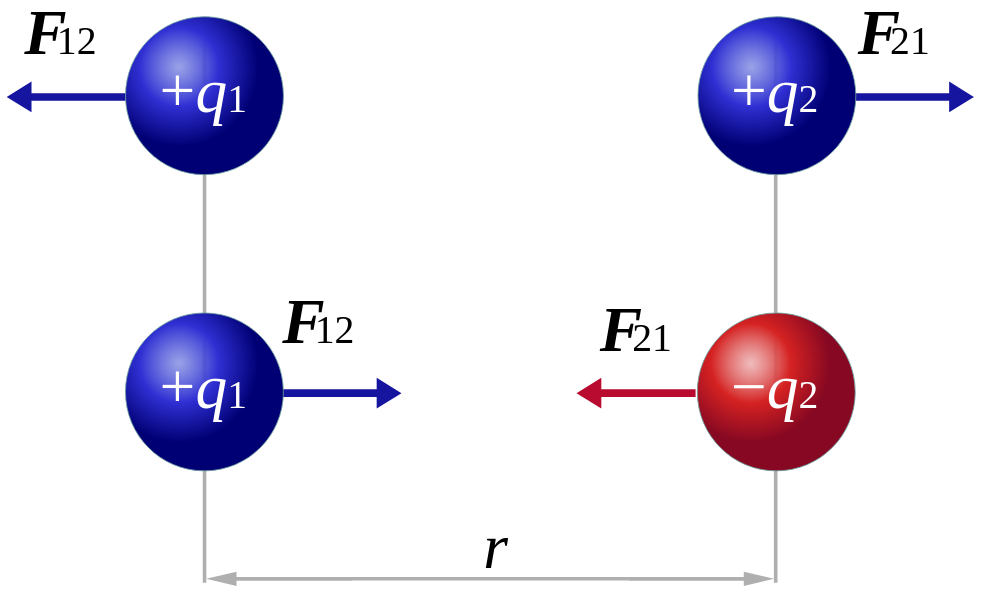
\includegraphics[width=0.5\linewidth]{imagens/ar2.png}
		\caption*{Fonte: Wikipedia (adaptada), original disponível em https://shorturl.at/kwB35}
	\label{fig:ar}
	\end{figure}

	\section{Partículas fundamentais}
	Se considerarmos o Big Bang como o início de tudo que existe no universo conhecido, sabemos que as primeiras partículas a se formarem foram aquelas que chamamos de \textbf{fundamentais} \cite{griffiths2020introduction} e entre elas citamos os quarks, elétrons, fótons e glúons, como pode ser visto na figura \ref{fig:particulaselementares}

\begin{figure}[H]
	\centering
	\caption{Modelo Padrão de partículas elementares}
	\vspace{0.25cm}
	\label{fig:particulaselementares}
	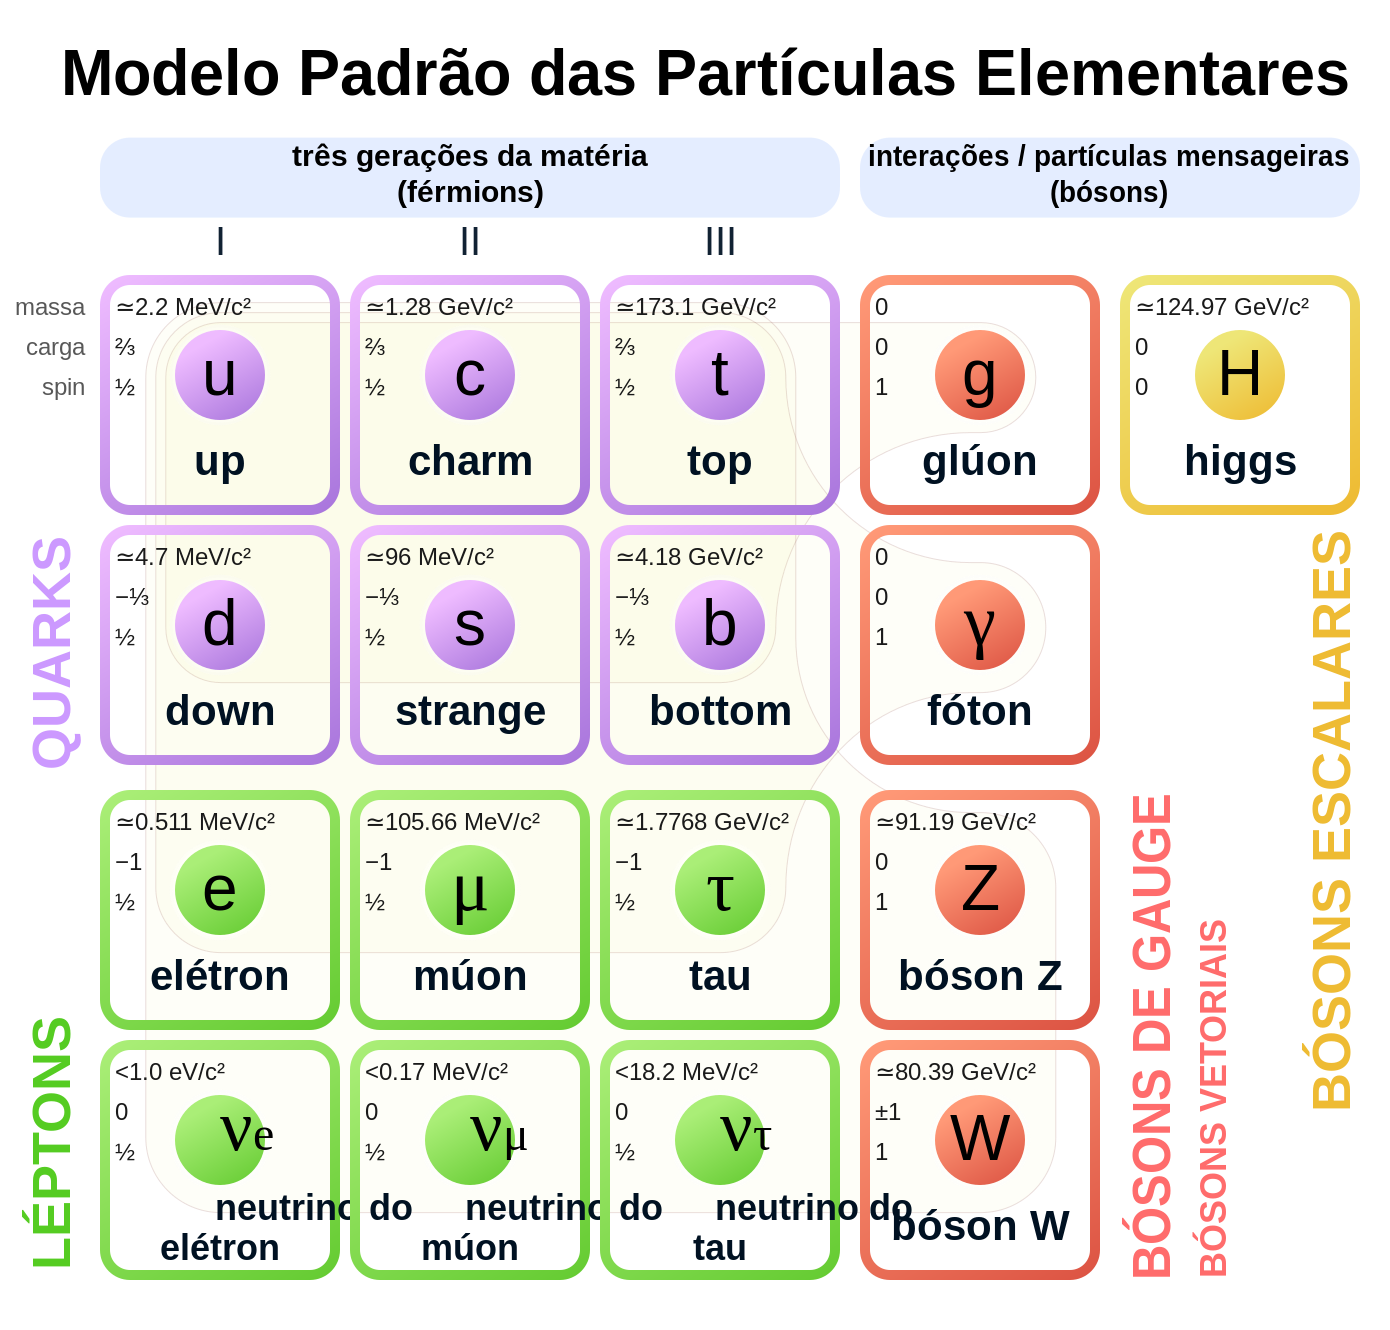
\includegraphics[width=0.75\linewidth]{imagens/boson2.png}
	\caption*{Fonte: Wikipedia, original disponível em https://shorturl.at/qwEOZ}
\end{figure}

A descrição completa da Figura \ref{fig:particulaselementares} está além do escopo primário deste livro, mas podemos analisar, sem grandes dificuldades, a composição detalhada de um próton, pois você deve lembrar-se que seis desses prótons formam o núcleo do magnífico carbono.

Não é tão complicado e siga o fio para entender claramente. Sabemos que o próton possui carga positiva com valor 1,6{$\cdot$}10{$^{-19}$} C \footnote{C é a unidade de carga chamada Coulomb} e massa aproximada de 1 u (ou massa atômica \cite{IUPAC+A00496+2019}) \footnote{1 u = 1,66 $\cdot$ 10$^{-24}$ g}. Estudos na área da Física de Alta Energia mostraram que o próton é formado por três quarks: dois quarks up e um quark down, unidos por um bóson chamado \textbf{glúon} Seguindo os dados presentes na Figura \ref{fig:particulaselementares}, cada quark up possui carga +2/3 e cada quark down possui carga -1/3. A soma simples dessas cargas resulta em 3/3, ou seja, 1. 

A manutenção desse sistema todo que mantém o próton íntegro é mediada pela \textbf{Força Nuclear Forte}, uma das forças elementares da Natureza e também a mais forte delas, embora atue apenas na escala nuclear.

De modo semelhante e com resultados dos mesmos estudos, um nêutron (com carga zero) é formado por um quark up e dois quarks down. A soma dessas cargas resulta em zero!

Muito bem! Já sabemos como se organizam as três partículas de mais fácil compreensão em átomos: prótons, nêutrons e elétrons. Mas precisamos entender como são produzidos átomos maiores, o que nos deixa com outra pergunta um tanto séria: conhecendo o Princípio de Repulsão das Cargas Elétricas, como é possível manter, por exemplo, dois prótons em um núcleo atômico? A resposta é composta duas partes:

\begin{enumerate}
	\item \textbf{A presença de nêutrons}. Sabemos que estas partículas são formadas por um próton e um elétron, mantidos unidos por uma entidade sem massa nem carga chamada \textbf{neutrino}. Uma das funções dos nêutrons no núcleo atômico é justamente afastar ligeiramente os prótons de outros prótons, como forma de diminuir a repulsão elétrica causada pela proximidade de partículas de mesma carga colocadas em uma distância tão pequena como as verificadas em escala nuclear.
	\item \textbf{A Força Nuclear Forte}: A força nuclear forte é uma das quatro forças fundamentais da natureza, responsável pela coesão entre os núcleos atômicos. Ela é responsável por manter os prótons e nêutrons unidos, apesar da repulsão eletromagnética entre os prótons, que são carregados positivamente. A força nuclear forte é muito mais forte que a força eletromagnética, sendo cerca de 100 vezes mais forte. No entanto, ela tem um alcance muito curto, de apenas cerca de 10$^{-15}$ metros. Isso significa que ela só é significativa em distâncias muito pequenas, como no interior do núcleo atômico.
	
	A força nuclear forte é mediada por partículas chamadas \textbf{glúons}. Os glúons são partículas elementares que não possuem massa. A força nuclear forte é responsável por ligar os quarks, que são as partículas elementares que compõem os prótons e nêutrons. A força nuclear forte é fundamental para a existência da matéria como a conhecemos. Ela é responsável pela formação dos átomos, das moléculas e das estrelas. Sem a força nuclear forte, o universo seria um lugar muito diferente, com átomos muito instáveis e sem a possibilidade de formar estruturas complexas.
\end{enumerate}

Para entendermos como essas partículas nucleares foram criadas, precisamos compreender que partículas maiores são sempre formadas a partir da junção ou fusão de partículas menores, e tal operação requer energia em quantidades incrivelmente altas, obtidas apenas em condições experimentais raras e caras, ou ainda em estrelas, principalmente aquelas presentes na chamada "Sequência Principal".

\section{Ciclo de Vida Estelar}\index{Ciclo de vida estelar}

Todas as estrelas conhecidas transitam pela chamada \textbf{Sequência Principal}, onde o núcleo estelar possui as condições de temperatura e pressão capazes de fundir Hidrogênio em Hélio, processo que exige temperatura próxima de 100 milhões K. Em função de sua massa, nosso Sol queimará todo seu Hidrogênio em Hélio durante um intervalo de tempo bastante elevado, por volta de 4 ou 5 bilhões de anos. Depois de esgotar seu combustível, o Sol passará por uma transformação radical e converter-se-á em uma estrela gigante vermelha, com capacidade nuclear para produzir Carbono e Oxigênio. Porém, para tanto, seu tamanho aumentará sobremaneira que inviabilizará a vida na Terra. Veja na Figura \ref{fig:HR} \cite{HR} a correlação entre cor e magnitude das estrelas.

\begin{figure}[h]
	\centering
	\caption{Diagrama de Hertzsprung-Russell}
	\vspace{0.25cm}
	\label{fig:HR}
	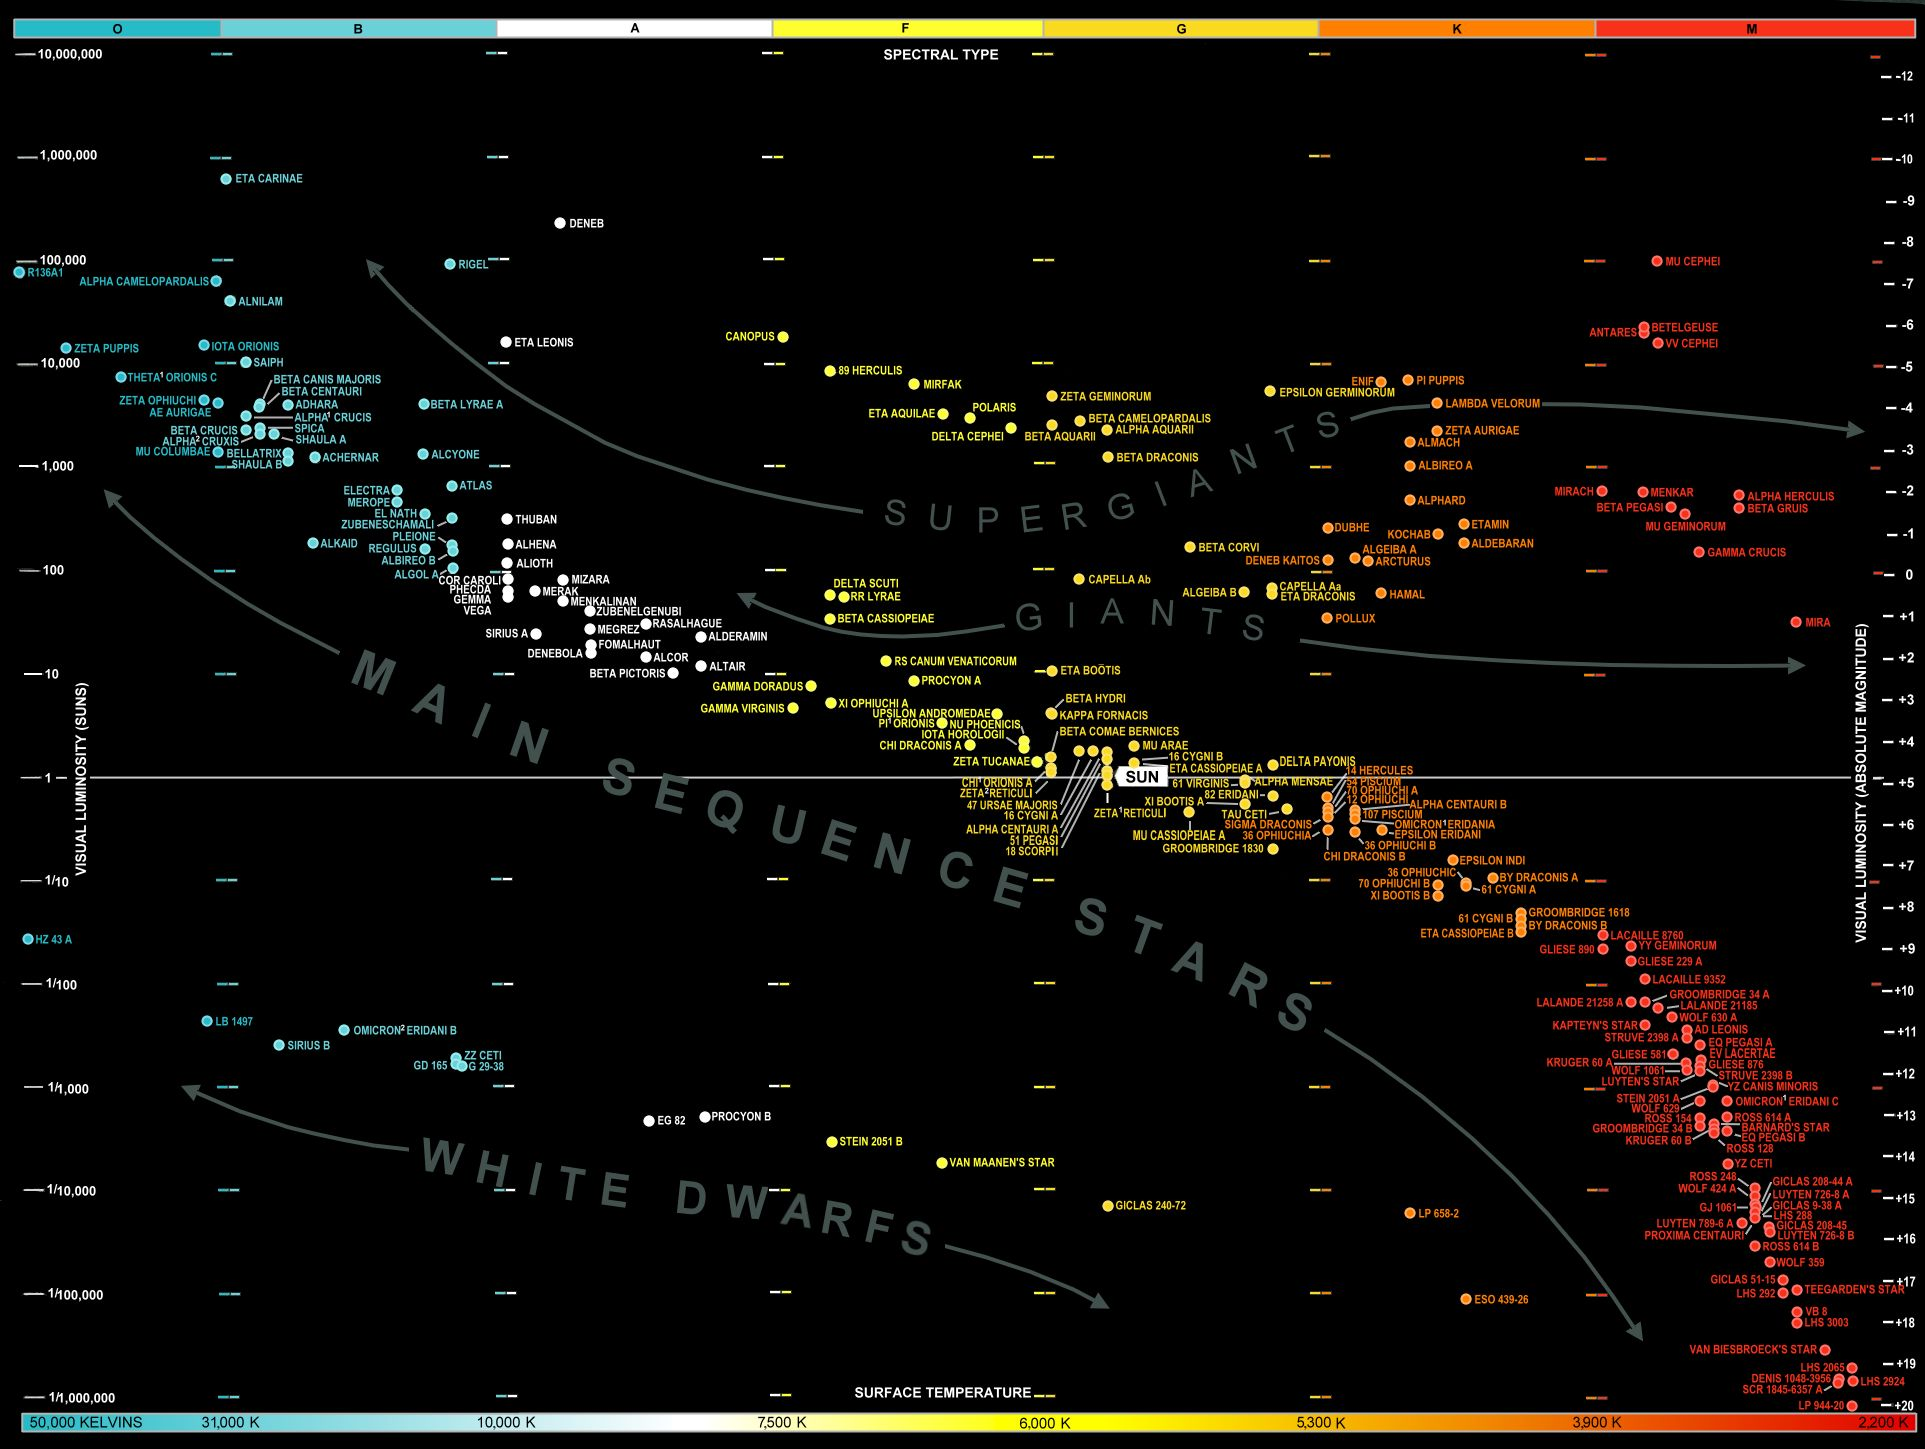
\includegraphics[width=1\linewidth]{imagens/diagrama-hr-completo.jpg}
	\caption*{Fonte: Scientific American, disponível em https://shorturl.at/dzELZ}
\end{figure}

O diagrama contém um grupo de estrelas, incluindo o Sol, que formam uma linha diagonal (parece mais uma curva sigmóide) que vai do lado superior esquerdo (com estrelas brilhantes e quentes) ao lado inferior direito (com estrelas menos brilhantes e "mais frias"). Essa diagonal é a chamada \textbf{Sequência Principal}. Estrelas mais brilhantes promovem reações de fusão mais rapidamente porque são mais massivas e, portanto, mais quentes.

O diagrama também mostra, na parte superior direita as chamadas \textbf{estrelas supergigantes}, que muitas vezes explodem como \textbf{supernovas}. A produção de Carbono, em estrelas mais massivas que o Sol, envolve temperaturas bem mais altas que em nosso Sol e ocorre em camadas mais profundas na estrela e o caminho em direção ao centro aumenta a temperatura e pressão cada vez mais, possibilitando a nucleossíntese de outros elementos químicos, até o Ferro. Elementos mais pesados que o Ferro são produzidos em processos extremos, como a explosão de supernovas, estrelas muito massivas que esgotam seu combustível e então explodem. Esse processo extremo espalha elementos químicos produzidos na explosão e, eventualmente, enriquece nuvens de gases e poeira na região do espaço onde o Sol e Terra se formaram. Assim, os elementos que aqui existem são originários da desintegração de outras estrelas.

\section{Nucleossíntese dos átomos de Carbono}
A vida no planeta Terra é baseada no elemento químico Carbono e por tal razão iniciamos nossa jornada a partir do ponto zero: como os átomos de Carbono são produzidos em processos estelares. Para que se tenha uma ideia da dimensão energética envolvida, a temperatura necessária atinge, aproximadamente, 10$^8$ K. Isso mesmo: cem milhões!

É um consenso que átomos de Carbono formaram-se, assim como outros elementos, através de violentíssimos choques causados por eventos que beiram o inimaginável, como a quase inacreditável temperatura citada anteriormente. Os pesquisadores \textbf{Subrahmanyan Chandrasekhar} e \textbf{William Alfred Fowler}, que desenvolveram - e comprovaram - essas ideias foram laureados com o Prêmio Nobel de Física em 1983 \footnote{Veja mais em https://www.nobelprize.org/prizes/physics/1983/summary/}, quase 30 anos após os estudos iniciais.

Estrelas com capacidade energética suficiente conseguem "fundir Carbono" \index{Nucleossíntese do Carbono}, usando uma terminologia muito frequente na área astronômica. As mais recentes concepções sobre a nucleossíntese do Carbono envolvem um processo conhecido como "Triplo Alfa". A expressão "fundir Carbono" significa um conjunto de reações nucleares que parte de átomos mais leves, como Hélio ou Berílio, para formar o núcleo do Carbono, por meio da fusão nuclear. Este método exige muita energia, e a produção de elementos mais pesados que o carbono requer ainda mais energia.

\section{O Processo Triplo Alfa}
Sabemos há um bom tempo que o núcleo do átomo de Carbono é composto por seis prótons e seis nêutrons, totalizando doze partículas. Repare que o nome do processo relaciona-se com uma partícula radioativa conhecida como radiação (ou partícula) alfa, que possui dois prótons e dois nêutrons, mas sem seus elétrons, o equivalente ao núcleo do átomo de Hélio. A união dessas partículas produzirá o núcleo do Carbono e caracteriza o Processo Triplo Alfa \index{Processo Triplo Alfa} \cite{TA}.

Analise a Figura \ref{fig:triploalfa} para melhor compreensão do processo, embora apresentado de modo bem simplificado.

\begin{figure}[h]
	\centering
	\caption{O Processo Triplo Alfa}
	\vspace{0.25cm}
	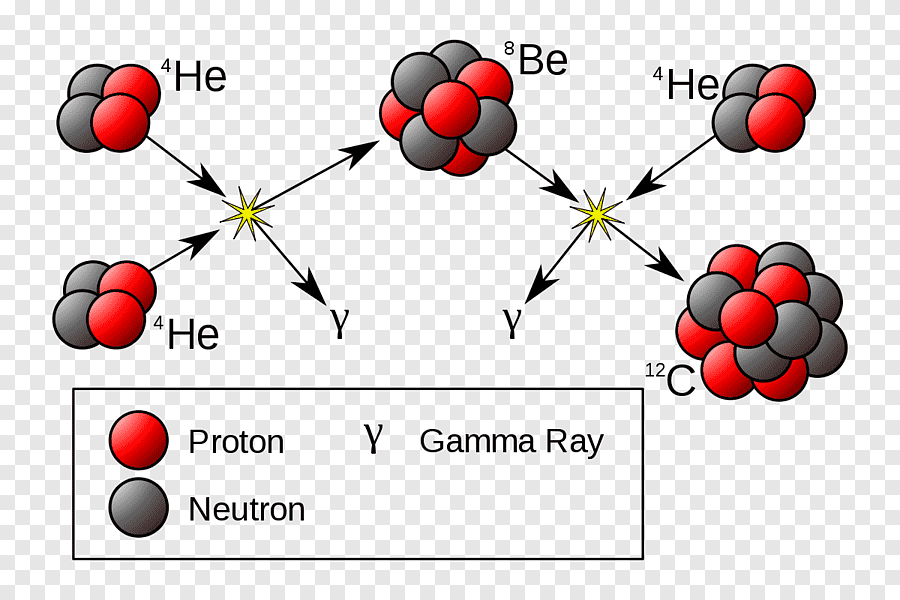
\includegraphics[width=0.75\linewidth]{imagens/ta.png} 
	\label{fig:triploalfa}
\end{figure}

O processo triplo alfa é uma reação nuclear de fusão que converte três núcleos de Hélio (partículas alfa) em um núcleo de Carbono. Este processo é responsável pela produção de Carbono no universo, e é um dos processos mais importantes na nucleossíntese estelar.

O processo triplo alfa ocorre em temperaturas muito altas, acima de 100 milhões de kelvin. Essas temperaturas são encontradas no núcleo das estrelas, onde o Hidrogênio é fundido em Hélio e ocorre em duas etapas:

\begin{enumerate}
	\item \textbf{Berílio-8}: Duas partículas alfa se fundem para formar um núcleo de Berílio-8. O Berílio-8 é um núcleo instável, que se decompõe em duas partículas alfa em cerca de $10^{-16}$ segundos.
	\item \textbf{Carbono-12}: Uma partícula alfa se funde com um núcleo de Berílio-8 para formar um núcleo de Carbono-12, estável. O processo é um processo altamente eficiente, liberando cerca de 7,2 milhões de elétron-volts \footnote{O elétron-volt (eV) é uma unidade de medida de energia. É utilizado principalmente na física de partículas e na física atômica. Um elétron-volt é a quantidade de energia cinética ganha por um único elétron quando acelerado por uma diferença de potencial de um Volt.} de energia. Esta energia é usada para sustentar a fusão nuclear das estrelas.
\end{enumerate}

O processo triplo alfa foi um processo importante para a vida na Terra, uma vez que o Carbono é um elemento essencial para a vida neste planeta, e o processo triplo alfa é responsável pela produção de Carbono no universo. O Carbono é um elemento mais pesado que o Hélio, e sua produção marca o início da produção de elementos mais pesados nas estrelas.

A partir desse momento, o átomo de Carbono formado em aglomerados de gás e poeira, lentamente agrupa-se com outros incontáveis átomos para formar, por exemplo, nosso planeta azul chamado Terra. O planeta conta, agora, com muitos tipos de elementos químicos e as diversas modificações sofridas pelo planeta em tempos remotos acabaram resultando em muitas substâncias conhecidas hoje, mas a formação de biomoléculas é um assunto complexo o suficiente para ser tratado em separado, em outro ponto deste livro.
	
\chapter{Ascenção e queda da Teoria da Força Vital}
\begin{mdframed}[backgroundcolor=orange!20,linewidth=0pt,roundcorner=10pt]
\minitoc
\end{mdframed}
O tempo passou e diversos apaixonados pela experimentação viviam a expectativa de criar novas substâncias, ou então simplesmente obter algo como o utópico Elixir da Vida Eterna ou então o milagre da (hoje chamada) transmutação, na esperança vã de transformar qualquer metal em ouro. \index{Vitalismo}

Naturalmente, nenhum desses dois objetivos de muitos alquimistas foi alcançado, pois hoje sabemos que o corpo humano, por mais longevo que seja, não possui capacidade de persistir por pouco mais de 120 anos. Do mesmo modo, transformar um metal em ouro envolve complicados processos nucleares nem sempre efetuados com sucesso, mas tal conhecimento ainda não estava disponível aos alquimistas. De qualquer forma, o esforço desses pesquisadores permitiu o avanço, embora um pouco tímido, da Química como ciência experimental.

O magnífico Antoine-Laurent de Lavoisier, descobridor do Oxigênio, Hidrogênio e do Enxofre, lançou as bases da ciência baseada na absoluta necessidade de experimentação laboratorial e enunciou, por volta de 1777, a Lei de Conservação da Massa, na qual, em um sistema fechado, a massa total de reagentes e produtos permanece constante. Este enunciado ajudou John Dalton, no começo do século 19, a elaborar seu modelo atômico.

\begin{figure}[h]
	\centering
	\caption{Antoine-Laurent de Lavoisier e Marie-Anne Pierretti Paulze}
	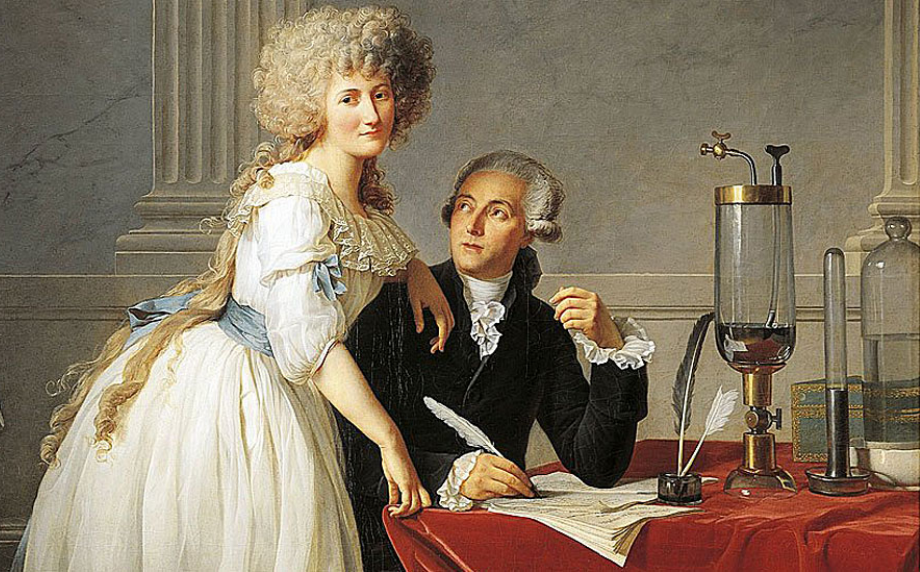
\includegraphics[width=0.85\linewidth]{imagens/figura 4.png} 
	\caption*{Fonte: BBC News Brasil, disponível em https://shorturl.at/owP17}
	\label{fig:wrapfig}
\end{figure}


\section{Teoria da Força Vital ou Vitalismo}
Muitos pesquisadores e entusiastas da ciência realizavam todo tipo de experimentação, o que criou, por exemplo, o ofício de perfumista. A curiosidade os levava a analisar diversos materiais e organismos em busca de sua composição e, por causa de empreitadas assim, muitas substâncias foram descobertas, inclusive com aplicações médicas, mas tudo a partir daqui esbarrava em uma barreira até então intransponível: não era possível produzir artificialmente uma substância de origem vegetal ou animal, e apenas tais organismos possuíam uma misteriosa \textbf{força vital} \index{Força vital} que os permitia produzir tais substâncias.

Naquele momento da história, definia-se Química Orgânica como \textbf{a parte da Química que estuda substâncias obtidas de organismos vivos}, os portadores da Força Vital. Mas o tempo passou novamente e chegou-se em 1828, na Alemanha.

\section{Salve, Wöhler!}
A Química possui muitos nomes de destaque ao longo da história, como o próprio Lavoisier, Berzelius, Van't Hoff, Grignard, entre muitos outros. O próximo nome de destaque saiu de sua terra natal para estudar com Berzelius, em Estocolomo. A Universidade de Göttingen, onde Friedrich Wöhler \index{Wöhler} tornou-se docente, é considerada um celeiro de grandes nomes da ciência, como Gauss, Fermi e Pauli.

\begin{figure}[h]
	\centering
	\caption{Friedrich Wöhler}
	%\vspace{0.25cm}
	\label{fig:wohler}
	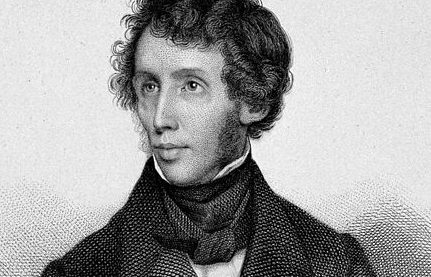
\includegraphics[width=0.5\linewidth]{imagens/wohler.jpg}
	\caption*{Fonte: Rincón Educativo, disponível em https://shorturl.at/notuK}
\end{figure}

Filho de pai veterinário e mãe filantropa, Wöhler era muito dedicado à ciência de modo geral, uma vez que sua atuação como químico não era a única de sua carreira, pois atuou também como obstetra, mas uma de suas atividades ajudou a mudar os rumos da Química Orgânica, até o momento restrita a substâncias extraídas de seres vivos, daí a origem do chamado Vitalismo.

Embora tenha sido considerado o estopim da derrocada do Vitalismo, este perdurou ainda por muitos anos devido, em parte, à dificuldade em aceitar algo radicalmente diferente e, podemos dizer, até certo ponto iconoclasta. O declínio do Vitalismo começou a ficar mais evidente em 1843, quando Hermann Kopp defendeu que a Síntese de Wöhler (uma delas) foi o ponto de partida para o abandono de teorias vitalistas. Mas qual seria essa tão marcante reação?

Na realidade, não foi apenas uma reação pontual, mas algumas que, combinadas em uma certa sequência, levaram à produção da ureia \index{Ureia}. Uma reação que pode ser considerada como representativa desse processo é apresentada na figura \ref{fig:ureia} a seguir.

\begin{figure}[h]
	\centering
	\vspace{0.5cm}
	\caption{Uma das etapas da síntese da ureia, por aquecimento do cianato de amônio.}
	\label{fig:ureia}
	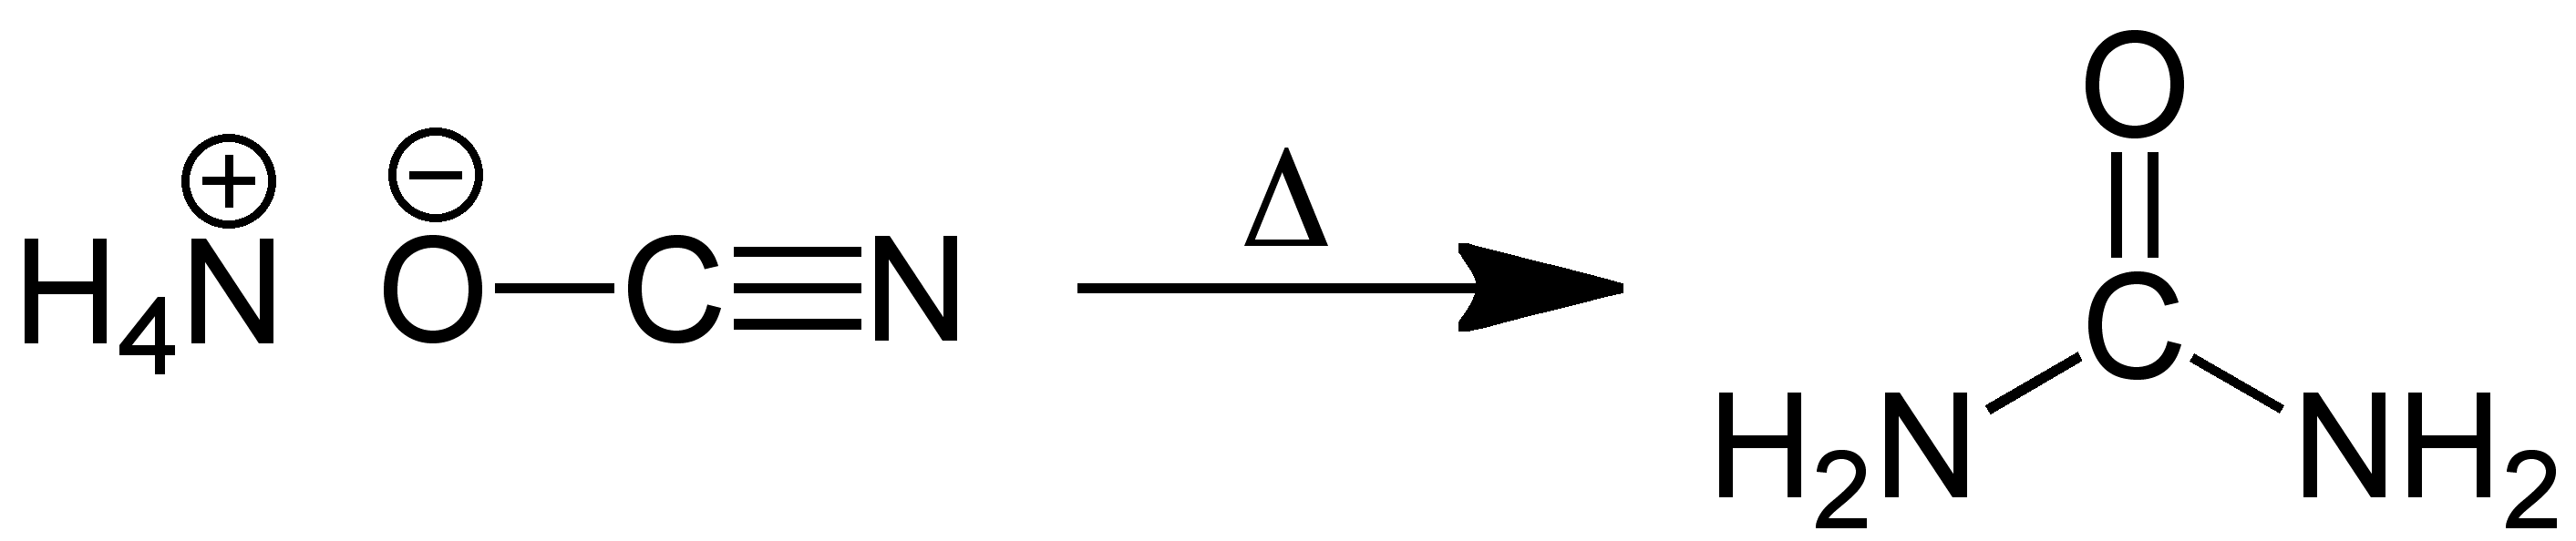
\includegraphics[width=0.7\linewidth]{imagens/Urea_Synthesis_Woehler.png}
	\caption*{Fonte: Autores}
\end{figure}

Esqueça, por um momento, que Wöhler era aluno de Berzelius, um dos mais fervorosos defensores do Vitalismo, este mortalmente ferido com a síntese de Wöhler. Qual foi uma consequência real de todo esse processo? A síntese de muitas outras substâncias orgânicas, como medicamentos, fertilizantes, entre muitos outros exemplos. Por razões estritamente pessoais, o autor deste livro exemplifica a molécula do taxol \index{Taxol} como uma consequência do feito de Wöhler, como pode ser visto na Figura \ref{fig:taxol}

\begin{figure}[h]
	\centering
	\caption{Estrutura do paclitaxel, uma substância polifuncional contendo as funções álcool, cetona, éter, amida e éster.}
	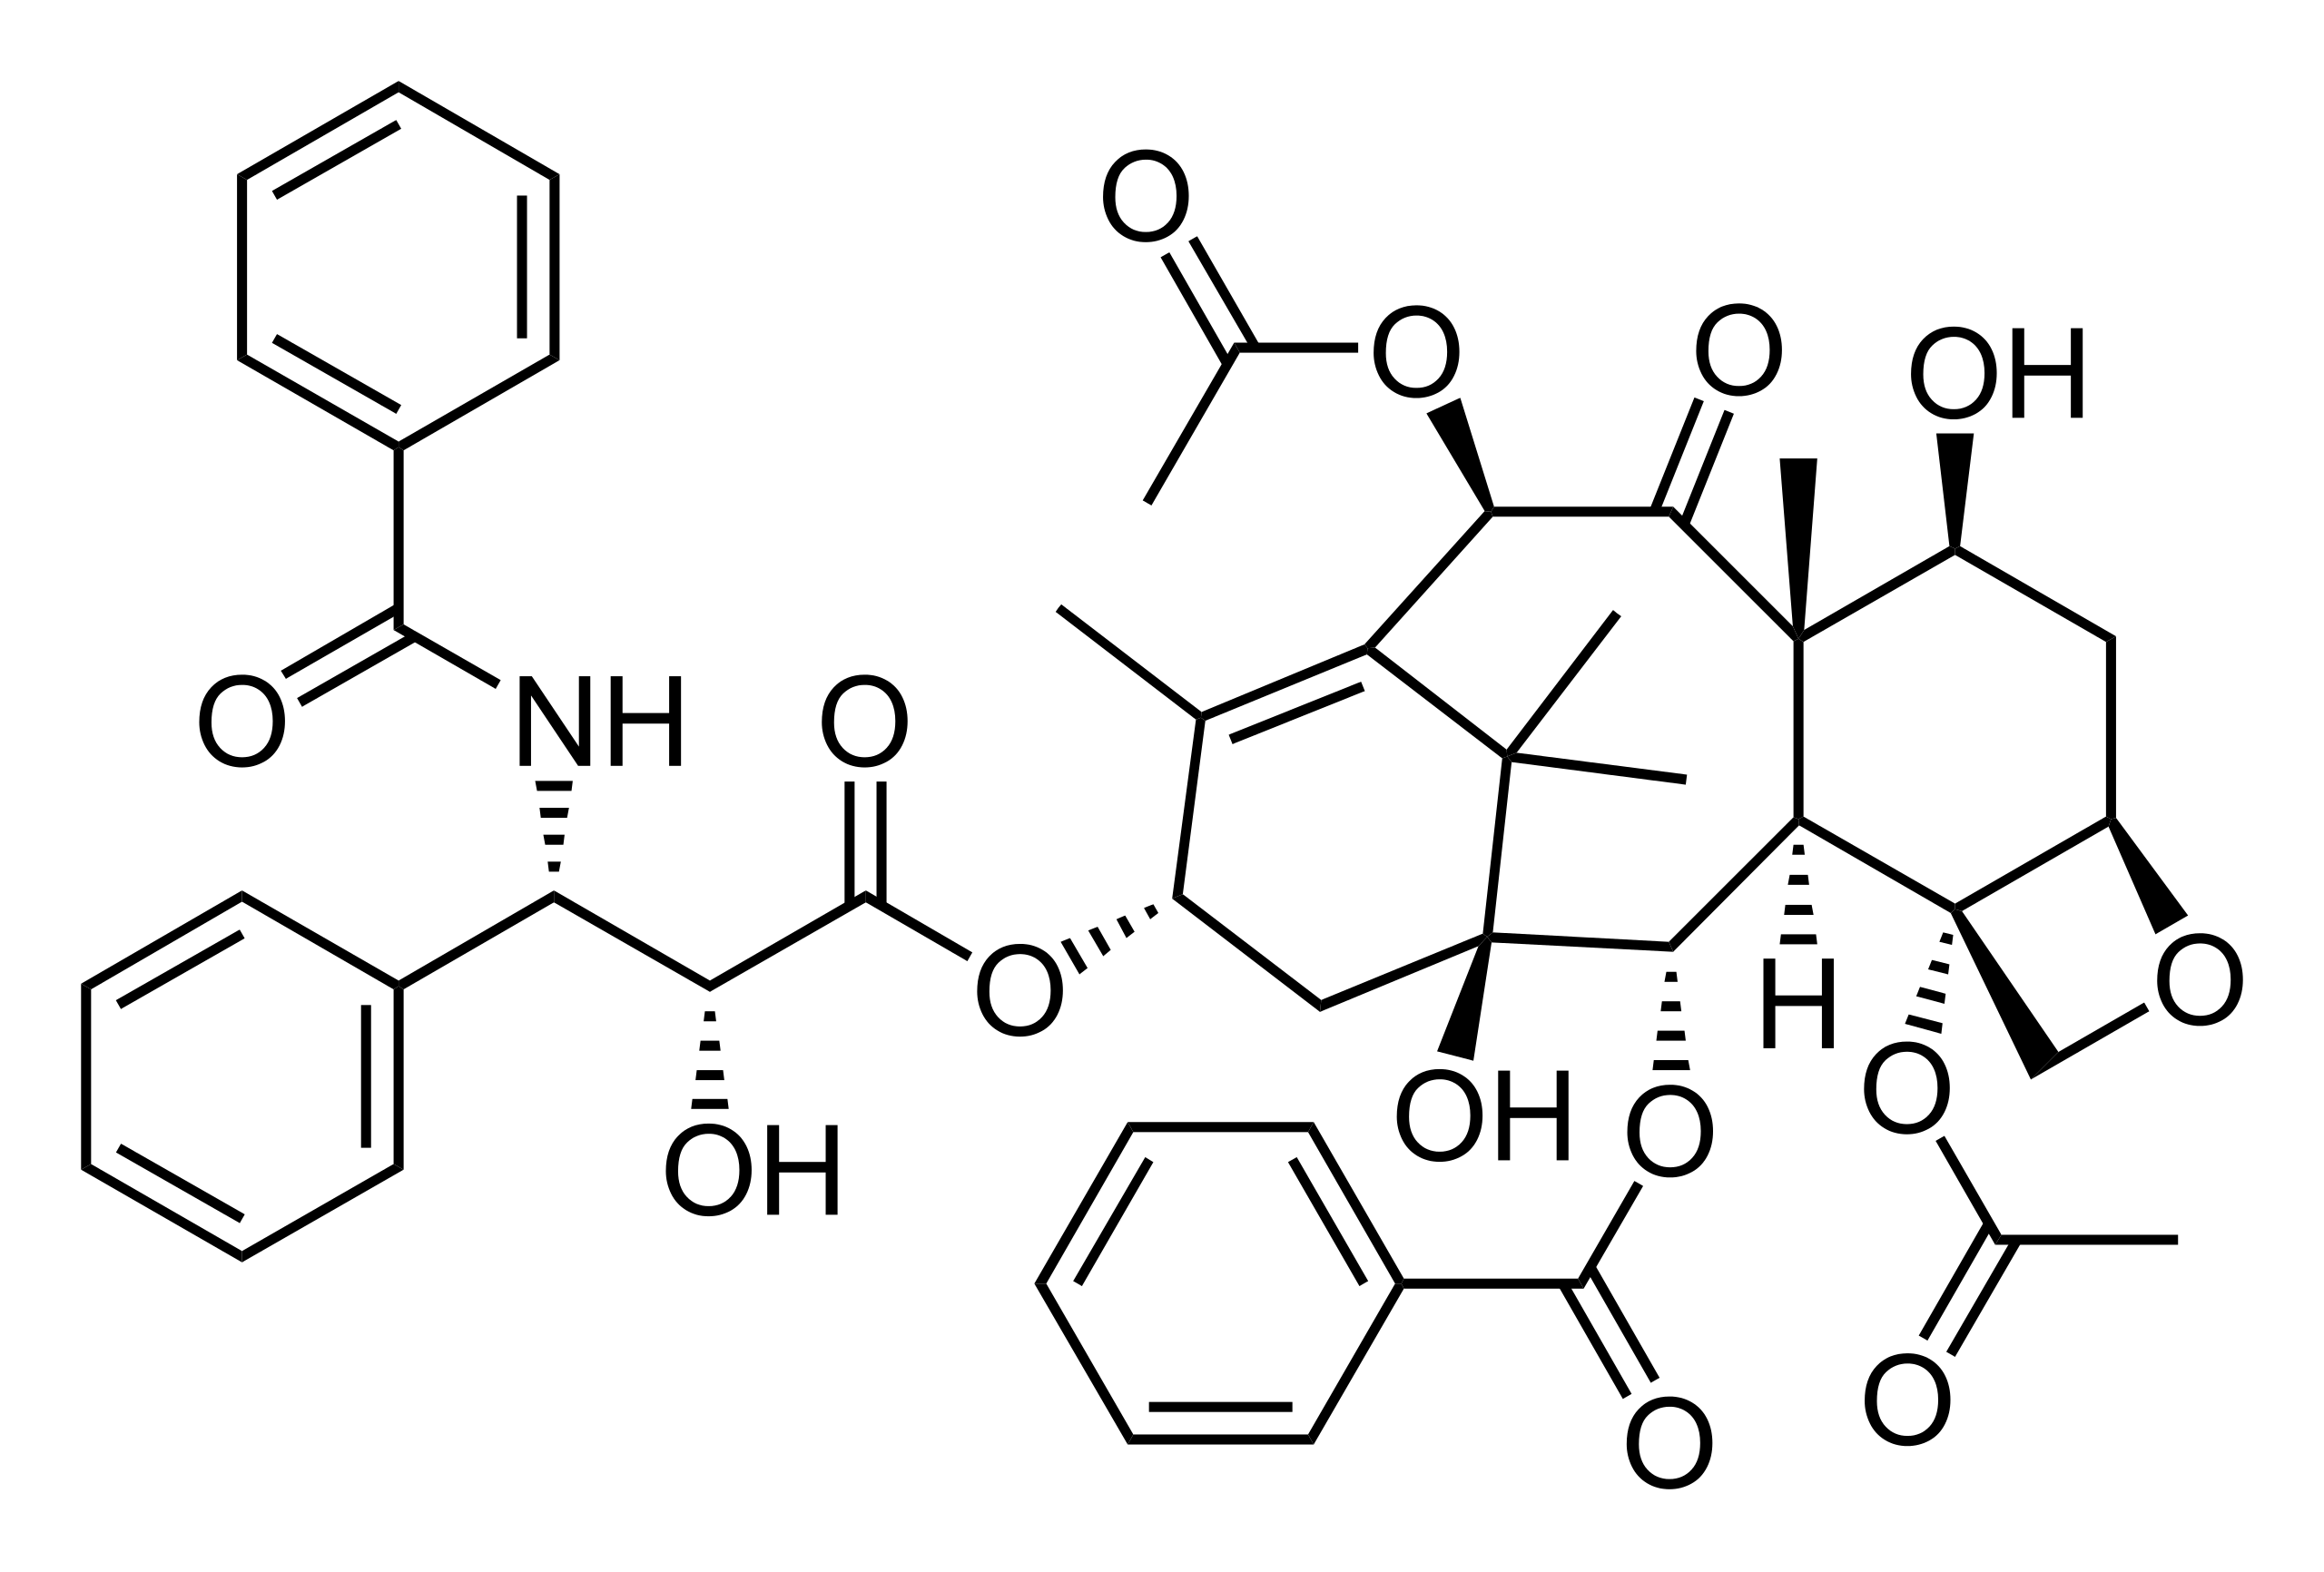
\includegraphics[width=0.5\linewidth]{imagens/Taxol.svg.png} 
	\label{fig:taxol}
	\caption*{Fonte: Autores}
\end{figure}


O que move a ciência é o questionamento: como alguém descobriu que essa molécula é encontrada nessa árvore em especial e ainda possui atividade antitumoral tão intensa? A resposta é simples e cristalina como água pura.

Na década de 1960, o National Cancer Institute (NCI), nos EUA, iniciou um programa ambicioso de \emph{screening}, ou seja, busca, por substâncias naturais com potencial atividade antitumoral e \textbf{foram coletadas amostras de mais de 35000 amostras de plantas diferentes}, no país todo. Perto de 10 anos após a coleta, uma substância chamada \textbf{paclitaxel}, com potencial ação antitumoral, foi encontrada e tornou-se um medicamento aprovado em 1992, quase 30 anos após o início do projeto de \emph{screening} \cite{paclitaxel}.

A ação do taxol está relacionada com a estabilização dos microtúbulos, impedindo que ocorra a despolimerização e causando a morte celular, uma vez que os microtúbulos são intimamente relacionados com a estabilidade da parede celular de células eucarióticas. Sua síntese foi muito aguardada e disputada no meio químico, pois foi necessário abater 38000 árvores para obter a quantidade de moléculas necessárias para tratar os 12000 pacientes dos ensaios clínicos in vivo.

Esteja onde estiver, Wöhler, esta conquista é sua!

\chapter{A ligação química Carbono-Carbono}
\begin{mdframed}[backgroundcolor=orange!20,linewidth=0pt,roundcorner=10pt]
	\minitoc
\end{mdframed}
Sabemos que um átomo é formado, de modo simplista, por duas regiões distintas em termos de tipo de partícula e também de densidade de partículas: o núcleo do átomo de carbono é bastante denso em termos de partículas e a chamada eletrosfera é rarefeita em quantidade de partículas.

A conexão que átomos fazem entre si ocorre na eletrosfera chama-se \textbf{ligação química}. Precisamos compreender, inicialmente, como os elétrons ficam dispostos nessa região e também o que é necessário para que esses elétrons mantenham-se próximos a outros elétrons que estão localizados em outros átomos.

As propostas de organização da eletrosfera atômica iniciaram-se com as revolucionárias ideias de \textbf{Ernest Rutherford}, como resultado dos experimentos da espalhamento de partículas alfa, realizados no icônico Laboratório Cavendish \footnote{Veja aqui o site do Laboratório Cavendish: https://www.phy.cam.ac.uk/}, na Universidade de Cambridge, no Reino Unido. Embora fossem revolucionárias, as ideias de Rutherford sobre a eletrosfera eram incompatíveis com conceitos sólidos a respeito de Eletromagnetismo.

Torna-se necessário analisar como ocorre a conexão entre dois átomos por meio de orbitais atômicos e, sabendo que elétrons ficam em orbitais, é importante que saibamos como se dará a aproximação e como ficam esses orbitais após a conexão entre os dois átomos. Torna-se necessário agora entender rapidamente o modelo atômico apoiado em conceitos da Mecânica Quântica.

Atualmente, a eletrosfera do átomo é organizada em níveis de energia, subníveis e, finalmente, \textbf{orbitais} \index{orbitais}, onde localizam-se os elétrons. Tecnicamente e de acordo com a IUPAC, \textbf{orbital é a função de onda monoeletrônica obtida pela solução da Equação de Schrödinger para um átomo \footnote{O tratamento matemático necessário para plena compreensão deste assunto está além do escopo deste livro e sugerimos a consulta a textos especializados em Mecânica Quântica.}}. A Figura \ref{fig:orbitais} mostra um quadro bem interessante a respeito de orbitais.

\begin{figure}[h]
\centering
\vspace{0.25cm}
\caption{Subníveis dos tipos \textbf{s}, \textbf{p}, \textbf{d} e \textbf{f}, com seus respectivos orbitais.}
\label{fig:orbitais}
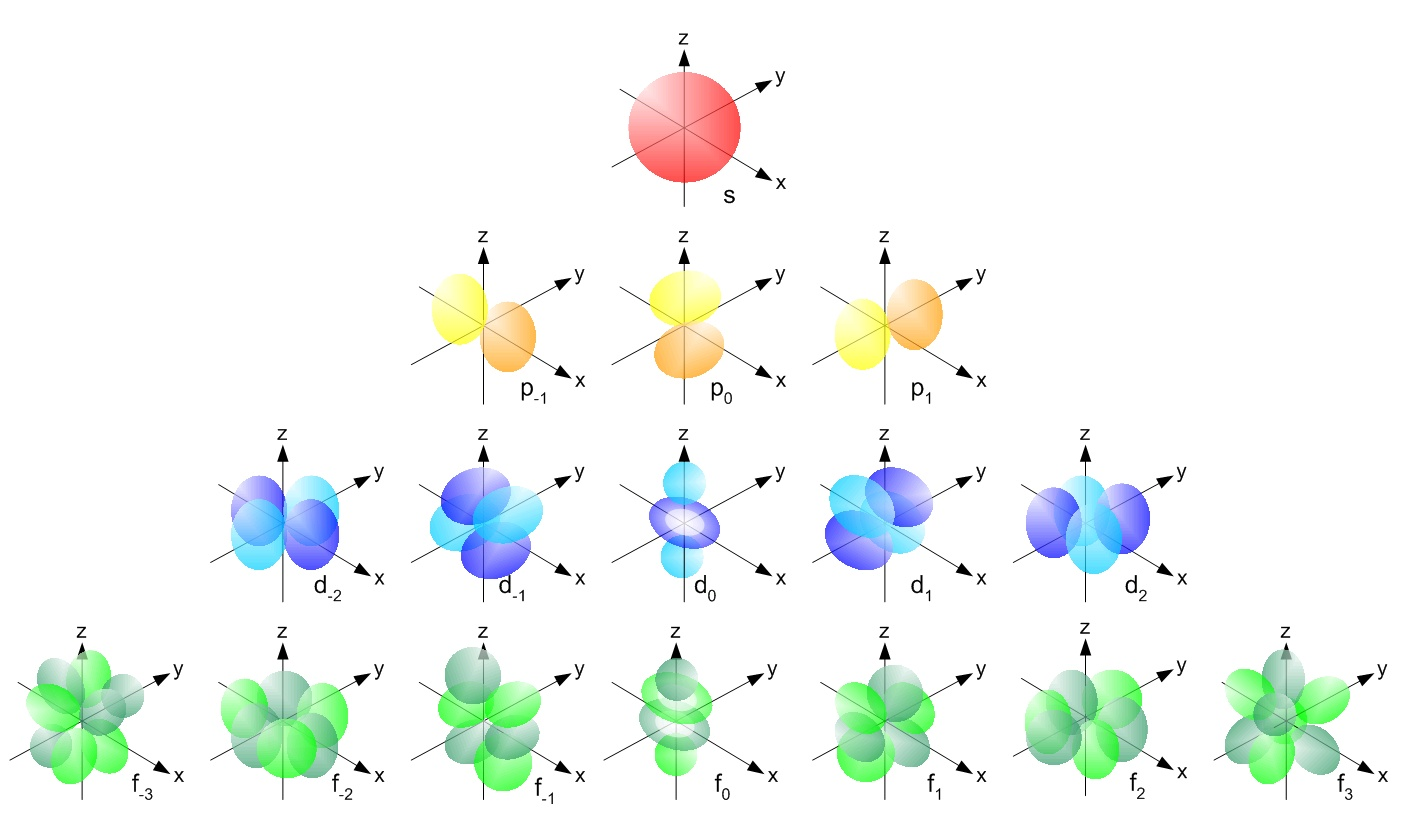
\includegraphics[width=1\linewidth]{imagens/all_orbitals.jpg}
\caption*{Fonte: Wikipedia, disponível em https://shorturl.at/eNY27}
\end{figure}

Cada parte colorida da Figura \ref{fig:orbitais} indica as regiões onde elétrons podem ser encontrados. O subnível s, que aparece na primeira linha da figura, é formado por apenas um orbital de forma esférica e os dois elétrons que esse orbital pode acomodar (assim como todos os demais orbitais) podem ocupar qualquer posição dentro da esfera. Uma evolução às ideias de Bohr, considerando a eletrosfera era unidimensional, as formas refletem a construção do modelo a partir das contribuições de Erwin Schrödinger e suas funções de onda, permitindo ao elétron ocupar determinadas regiões no espaço, mapeadas por coordenadas espaciais, chamadas de \textbf{números quânticos}. A segunda linha da figura apresenta o chamado subnível p, composto por três orbitais orientados em um sistema tridimensional e cada orbital é indicado de acordo com o eixo de orientação no qual se encontra: px, py e pz. Vale o mesmo raciocínio para os demais orbitais, mas nosso foco será no carbono.

\section{Números quânticos}
Conceitualmente e de modo simplificado, os números quânticos conhecidos por \textbf{principal}, \textbf{angular} e \textbf{magnético} definem, respectivamente, o tamanho, o formato e a orientação de cada orbital no espaço. 

O número quântico principal, representado pela letra \textbf{n} define o tamanho do orbital e está relacionado diretamente com o conceito anterior de \textbf{camada eletrônica}. Na Classificação Periódica dos Elementos (CPE) podemos observar a existência de sete períodos (ou linhas horizontais), diretamente relacionados com os sete níveis de energia conhecidos atualmente. Assim, um elemento presente no quinto período da CPE utiliza 5 níveis de energia para distribuir seus elétrons. O modo como tais elétrons são distribuídos em subníveis será visto mais adiante.

O formato do orbital é determinado pelo número quântico \textbf{angular} (chamado em alguns textos por secundário), representado pela letra \textbf{l} e está relacionado com o novo conceito de \textbf{subníveis}, ou cada uma das divisões de um dado nível de energia. Cabe aqui um esclarecimento muito importante: \textbf{subníveis são conjuntos de orbitais}. São utilizados atualmente, para os elementos conhecidos, quatro subníveis distintos e identificados pelas letras \textbf{s} (sharp, l = 0), \textbf{p} (principal, l = 1), \textbf{d} (diffuse, l = 2) e \textbf{f} (fundamental, l = 3).

Cada subnível também pode ser identificados por números e o número de orbitais em cada subnível é determinado por uma equação simples:

\begin{equation}
    m = 2\cdot l+1
    \label{eqn:orbitais}
\end{equation}

A equação \ref{eqn:orbitais} introduz o terceiro número quântico \textbf{m}, chamado de \textbf{magnético} e indica a orientação espacial de cada orbital em um dado subnível. Deste modo, quando falamos de um elétron localizado no quarto nível de energia (n = 4) e com número quântico angular com valor 2 (l = 2), temos possíveis 5 orbitais e, naturalmente, o mesmo número de orientações espaciais, e os valores numéricos que indicam esses orbitais estão na faixa (-l, ..., 0, ..., +l), com aplicação da equação \ref{eqn:orbitais}.

Aplicando essas ideias na análise da Figura \ref{eqn:orbitais}, entendemos o motivo pelo qual temos apenas \textbf{um} orbital no subnível s, \textbf{três} orbitais no subnível p, \textbf{cinco} orbitais no subnível d e \textbf{sete} orbitais no subnível f.

O chamado \textbf{Princípio da Exclusão de Pauli} \cite{massimi2005pauli} estabelece que dois elétrons não podem apresentar o mesmo conjunto de números quânticos e, portanto, cada orbital pode acomodar \textbf{apenas e tão somente dois elétrons}. Mas por que dois e não um, três ou outro número? Simples: é necessário um quarto grau de liberdade chamado \textbf{spin}, para explicar o comportamento de elétrons em determinados subníveis. Entenda o termo, de forma simples, como sendo a rotação do elétron em torno de seu próprio eixo. Como existem apenas duas direções possíveis para a rotação em torno de um eixo, só exitem dois valores de spin e justifica-se a capacidade máxima de \textbf{dois elétrons em cada orbital}.

\begin{figure}[h]
\centering
\caption{Representação esquemática do spin eletrônico}
\vspace{0.25cm}
\label{fig:spin}
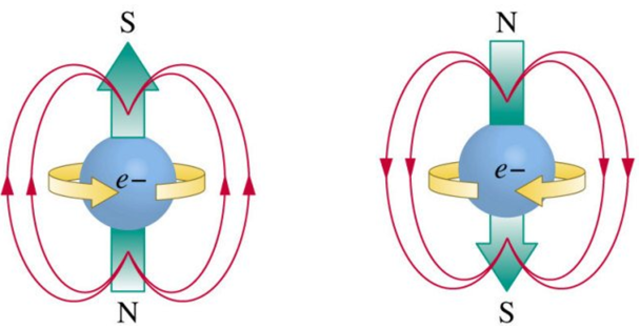
\includegraphics[width=0.5\linewidth]{imagens/spin.png}
\caption*{Fonte: Wikimedia Commons, disponível em https://shorturl.at/jEFL2}
\end{figure}

Conforme pode ser observado na Figura \ref{fig:spin}, o movimento de rotação do elétron (indicado pela seta circular de cor amarela na posição central de cada elétron) tem como consequência a geração de um \textbf{campo magnético} em cada elétron. Uma vez que os movimentos de rotação são opostos, os campos magnéticos gerados também são opostos entre si e isso os atrai. Não há como inserir um terceiro elétron em cada orbital por causa da repulsão que seria gerada por um ou outro elétron já existente no dado orbital.

\section{O conceito de hibridização}
Uma ligação química do tipo \textbf{covalente} é formada pelo compartilhamento de ao menos um elétron de um átomo com outro átomo. Para formar essa ligação, é necessário que um átomo possua um orbital semi-preenchido (com apenas um elétron) em seu subnível mais energético. A Figura \ref{fig:hibridacao_traduzida} mostra, na primeira linha, os subníveis do átomo de carbono e como seus elétrons distribuem-se nos subníveis. Repare que o subnível 2p possui três orbitais e apenas dois destes estão semi-preenchidos. Assim, o carbono forma apenas 2 ligações covalentes, contrariando o conhecimento secular estabelecido por Kekulé.

Como explicar a tetravalência do átomo de Carbono (capacidade de formar 4 ligações químicas)? Precisamos encontrar uma solução para obter um conjunto de \textbf{quatro orbitais semi-preenchidos}, mas o modo como a distribuição eletrônica do Carbono se apresenta não permite a existência dos quatro orbitais semi-preenchidos. Existe uma outra variável nesse problema: o mais simples dos hidrocarbonetos, chamado \textbf{metano} e com fórmula \textbf{\ce{CH4}}, possui 4 ligações covalentes simples e todas são quimicamente equivalentes, conforme pode ser visto na Figura \ref{fig:metanodetalhado}, ao lado direito. Nosso problema relacionado com as ligações químicas no átomo de Carbono aumentou.

\begin{figure}[H]
	\centering
	\caption{Detalhes estuturais do hidoarboneto chamado \textbf{metano} (\ce{CH4})}
	\vspace{0.5cm}
	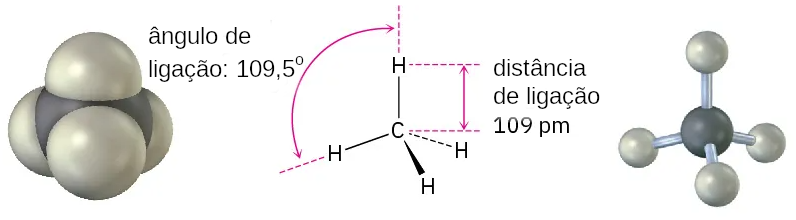
\includegraphics[width=0.8\linewidth]{imagens/metano_detalhado.png}
	\label{fig:metanodetalhado}
	\caption*{Fonte: LibreTexts (adaptada), disponível em https://shorturl.at/nzLTX}
\end{figure}

Esse problema, e sua solução, é muito importante na Química Orgânica e usaremos uma figura com linguagem visual diferente para deixar o conceito de \textbf{hibridização} o mais claro possível. 

\begin{figure}[H]
	\centering
	\caption{Esquema visual da formação de orbitais híbridos do átomo de Carbono}
	\vspace{0.5cm}
	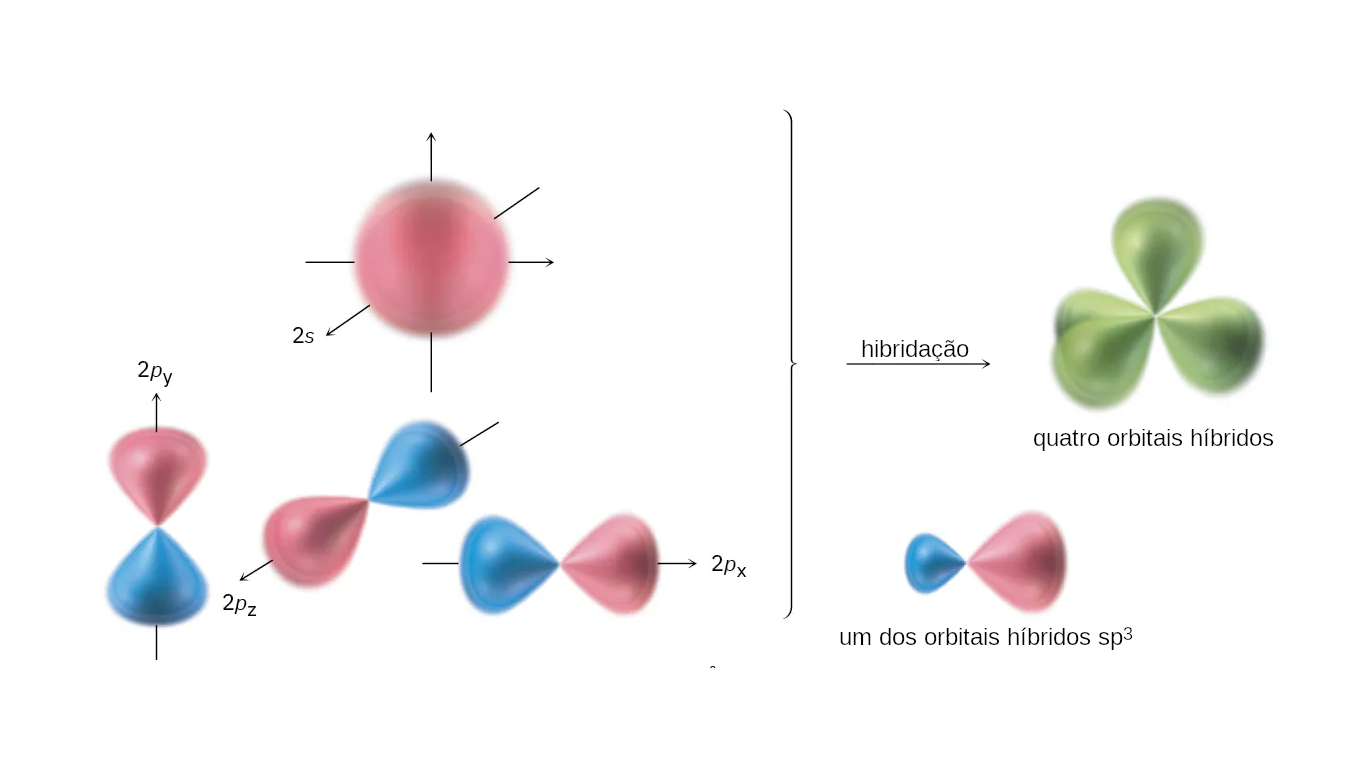
\includegraphics[width=1\linewidth]{imagens/hibridacao_visual_traduzida.png}
	\label{fig:hvt}
	\caption*{Fonte: LibreTexts (adaptada), disponível em https://shorturl.at/nzLTX}
\end{figure}

O mecanismo envolvido neste processo passa por uma combinação linear de orbitais \textbf{puros} \footnote{Usamos aqui a expressão \textbf{puro} para indicar um orbital não combinado} para formar orbitais \textbf{híbridos}, cuja composição e forma depende de quantos e quais orbitais puros foram combinados. Proposto por Linus Pauling em 1931 \cite{pauling}, o mecanismo chamado hibridização permite a existência de orbitais híbridos iguais que formam as quatro ligações químicas equivalentes no metano.

\begin{figure}[h]
\centering
\caption{Promoção eletrônica no átomo de Carbono}
\vspace{0.25cm}
\label{fig:fundexcit}
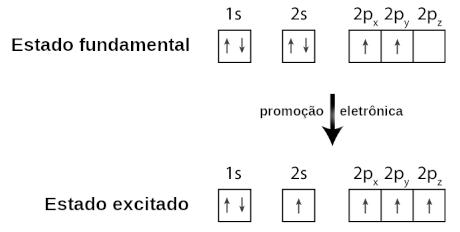
\includegraphics[width=0.7\linewidth]{imagens/fund_excit.png}
\caption*{Fonte: Wikimedia Commons (adaptada), disponível em https://shorturl.at/xyQX8}
\end{figure}

Analisando a Figura \ref{fig:fundexcit}, observamos o ponto central do processo de hibridização: a formação de orbitais \textbf{degenerados} (com mesmo conteúdo energético) através da promoção eletrônica e combinação linear dos subníveis 2s e 2p no átomo de Carbono. Uma configuração eletrônica chamada de \textbf{fundamental} é aquela que segue estritamente o \textbf{Princípio de Aufbau} ("construção", traduzido do idioma alemão e usado para a obtenção das configuraçoes eletrônicas de átomos) \cite{aufbau}; aquela que difere de algum modo da configuração do estado fundamenal é chamada de configuração \textbf{excitada}.

\begin{figure}[h]
\centering
\caption{Formação de orbitais híbridos no átomo de carbono}
\vspace{0.25cm}
\label{fig:hibridacao_traduzida}
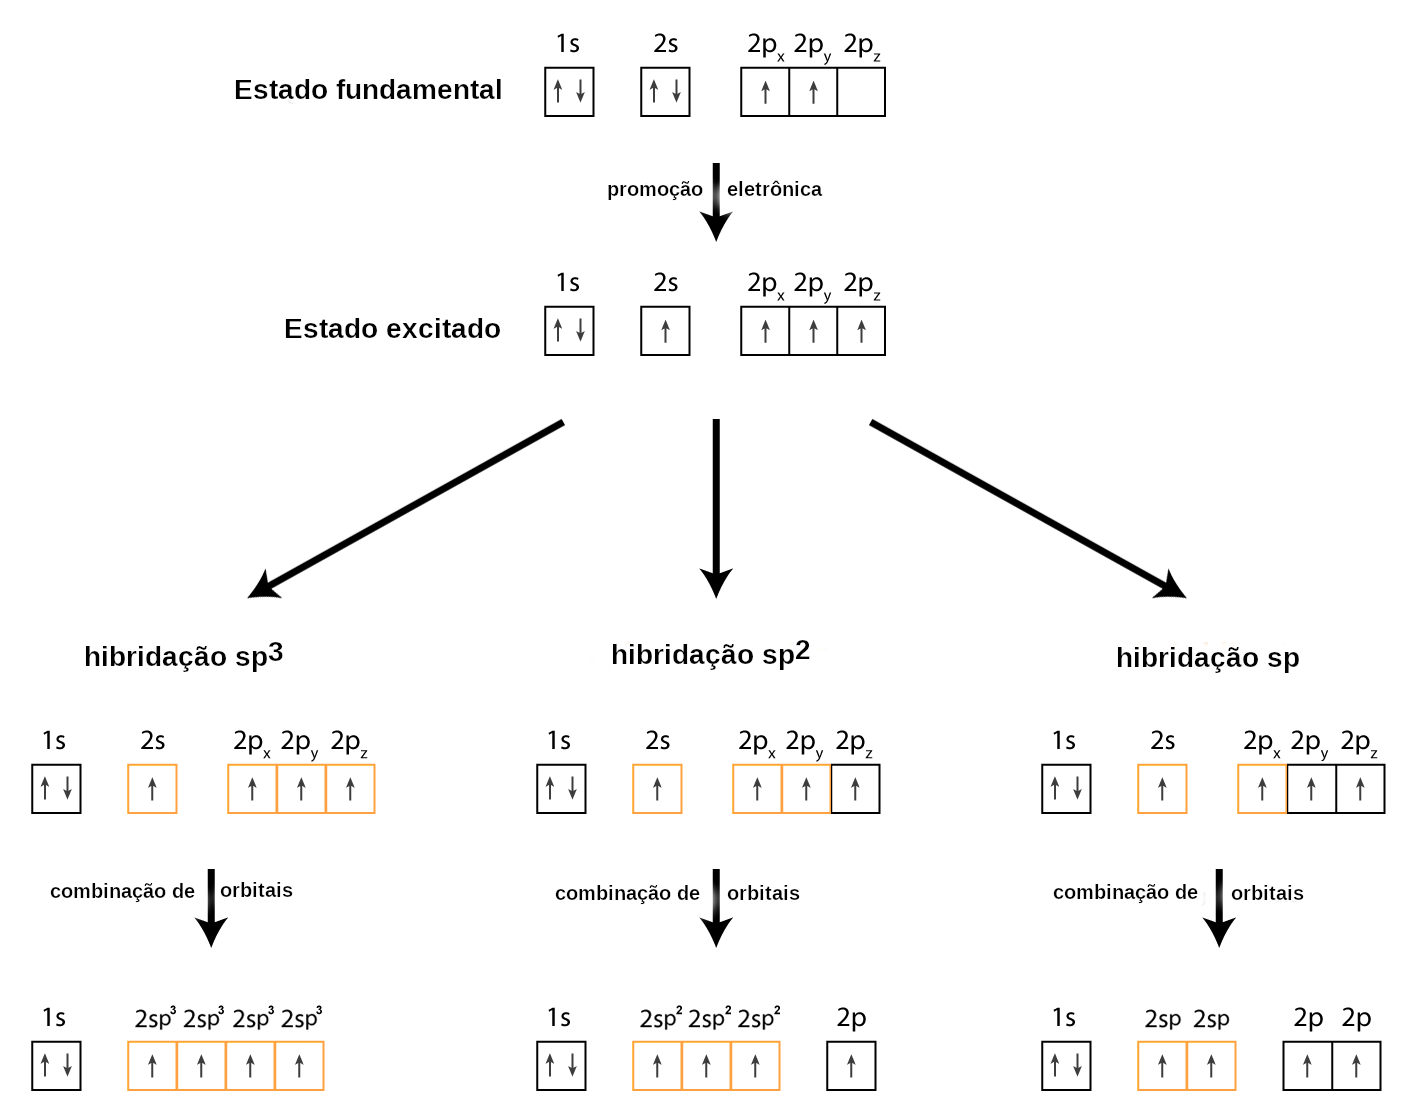
\includegraphics[width=1\linewidth]{imagens/Hybridization_of_carbon.png}
\caption*{Fonte: Wikimedia Commons (adaptada), disponível em https://shorturl.at/xyQX8}
\end{figure}

A partir da formação dos orbitais degenerados é possível, matematicamente, a existência de três combinações possíveis:

\begin{description}
	\item[\textbf{sp:}] o subnível 2s (contendo apenas um orbital) combina-se com apenas \textbf{um} dos orbitais p, restando dois orbitais puros e formando um conjunto de \textbf{dois orbitais híbridos sp}, separados entre si por 180\textcelsius.
	\item[\textbf{sp2:}] o subnível 2s (contendo apenas um orbital) combina-se com apenas \textbf{dois} dos orbitais p, restando um orbital puro e formando um conjunto de \textbf{três orbitais híbridos sp$^2$}, separados entre si por 120\textcelsius.
	\item[\textbf{sp3:}] o subnível 2s (contendo apenas um orbital) combina-se com todos os orbitais p, formando um conjunto de \textbf{quatro orbitais híbridos sp$^3$}, separados entre si por 109,5\textcelsius.
\end{description}

Os orbitais híbridos formados apresentam um arranjo espacial que justifica, em parte, a forma geométrica moléculas. A reatividade de uma molécula é explicada, em parte, por seu ambiente eletrônico, e o arranjo espacial de átomos contribui diretamente para a reatividade de substâncias orgânicas.

\section{A ligação sigma ($\sigma$)}

Uma ligação química, seja iônica ou covalente, pode ser considerada como o equilíbrio entre forças atrativas e repulsivas, conforme pode ser observado na Figura \ref{fig:dar}.

\begin{figure}[H]
	\centering
	\caption{Diagrama Lennard-Jones \cite{Lennard-Jones_1931} de forças atrativas e respulsivas na formação da molécula de H$_2$; válido para as demais ligaçãoes covalentes, respeitando a natureza de cada átomo. Observe que 1 pm = 10$^{-12}$ m}
	\vspace{0.5cm}
	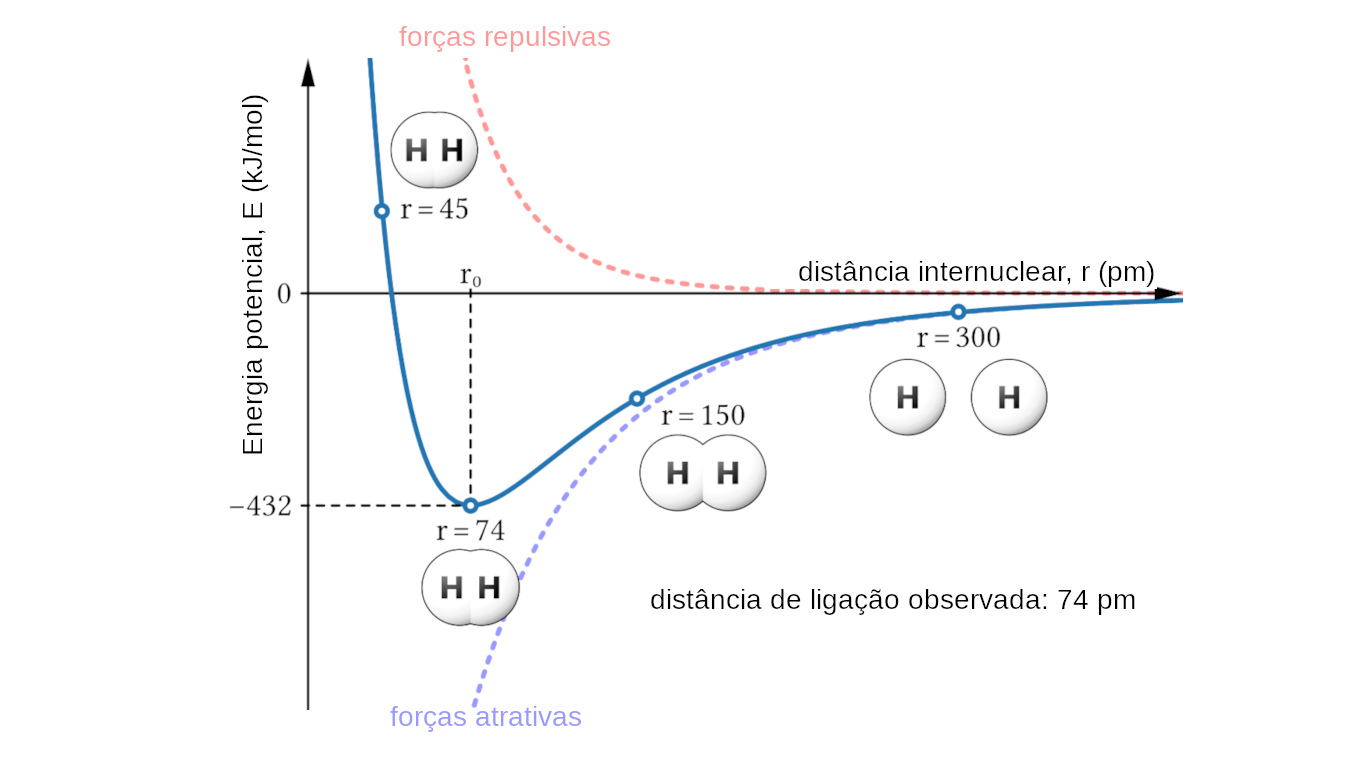
\includegraphics[width=1\linewidth]{imagens/dar.png}
	\label{fig:dar}
	\caption*{Fonte: Wikipedia (adaptada), disponível em https://shorturl.at/jDIL5}
\end{figure}

Precisamos analisar quatro regiões distintas no diagrama da Figura \ref{fig:dar}:

\begin{description}
	\item[300 pm:] nessa distância, a sobreposição dos orbitais atômicos de cada um dos átomos de Hidrogênio é praticamente nula e a estabilização que a ligação covalente traz aos átomos ainda não ocorreu. Nenhumas das forças, atrativa ou repulsiva, se manifesta a esta distância.
	\item[150 pm:] a essa distância a sobreposição dos orbitais dos átomos de Hidrogênio já ocorre em grande extensão e observa-se a predominância das forças \textbf{atrativas}, como pode ser observado pelo valor de energia negativa. 
	\item[74 pm:] nesse ponto tem-se a máxima sobreposição possível sem que perceba-se de algum componente repulsivo no sistema. A distância na qual ocorre essa sobreposição é chamada de \textbf{distância de ligação} e varia de acordo com os átomos envolvidos. 
	\item[45 pm:] em distâncias menores que 74 pm, os componentes de um dos átomos estão muito próximos daqueles do outro átomo e as forças repulsivas tornam-se muito maiores que as forças atrativas e o sistemas se desestabiliza completamente.  
\end{description}

Podemos, agora, tratar de ligações covalentes usando os conceitos de hibridização e orbitais moleculares. Uma ligação covalente do tipo $\sigma$ é aquela formada por meio da \textbf{sopreposição frontal de orbitais}, sejam puros ou híbridos. A Figura \ref{fig:sigma} apresenta à esquerda (a) uma representação que pode ser usada para compreensão do processo de formação da molécula do hidrocarboneto chamado \textbf{etano}, no qual as bolas azuis representam os átomos de Hidrogênio e o átomo de Carbono já se apresenta com seus quatro orbitais híbridos do tipo sp$^3$ em cor laranja.

O lado (b) da figura \ref{fig:sigma} mostra a molécula produzida a partir da sobreposição frontal de orbitais \textbf{s} puros dos átomos de Hidrogênio pelos orbitais híbridos \textbf{sp$^3$} dos átomos de Carbono, bem como a sobreposição frontal de orbitais híbridos de dois átomos de carbono distintos.

\begin{figure}[h]
\centering
\caption{Esquema simplificado de uma ligação $\sigma$, também chamada de ligação covalente simples.}
\vspace{0.25cm}
\label{fig:sigma}
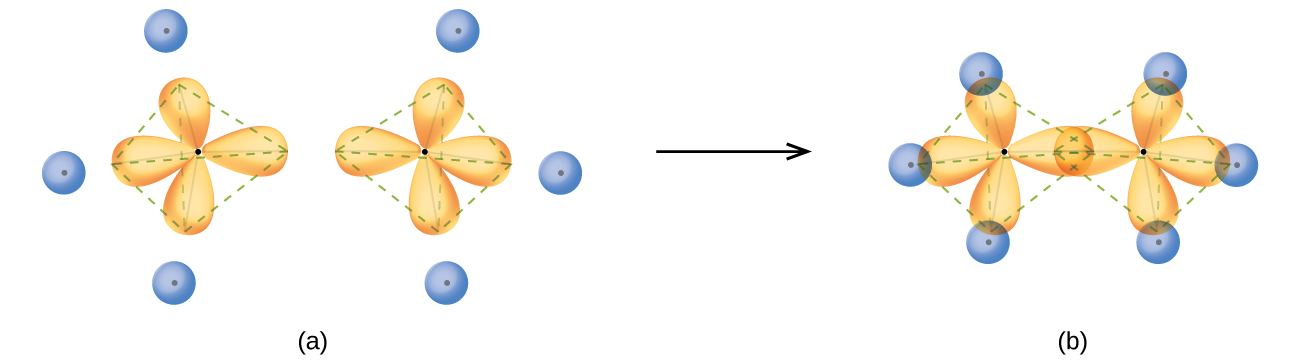
\includegraphics[width=1\linewidth]{imagens/sigma.jpg}
\caption*{Fonte: LabXchange, disponível em https://shorturl.at/zEVY6}
\end{figure}

A ligação $\sigma$ possui duas características importantes: \textbf{rotação} e \textbf{conformação}. Para exemplificar o conceito de rotação, usaremos o diagrama apresentado na Figura \ref{fig:om}.

\begin{figure}[h]
\centering
\caption{Exemplo de rotação da ligação sigma}
\vspace{0.25cm}
\label{fig:om}
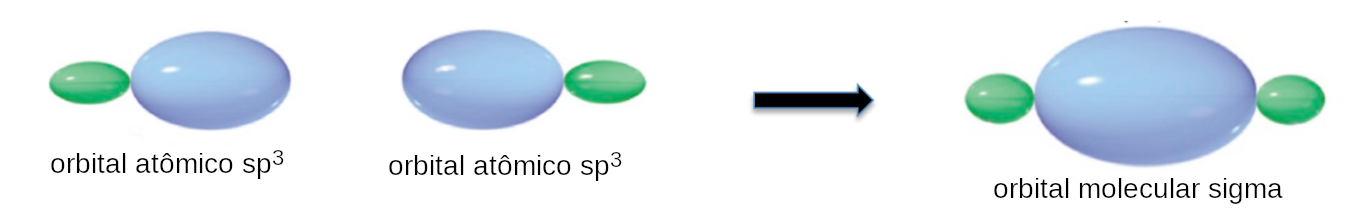
\includegraphics[width=1\linewidth]{imagens/om2.png}
\caption*{Fonte: Autores}
\end{figure}

Nosso foco está na parte \textbf{direita} da figura, onde vemos o orbital molecular formado pela sobreposição frontal de dois orbitais híbridos sp$^3$, também conhecido por ligação sigma. O ponto central da ligação que permite a rotação é a densidade eletrônica, representada pela área oval no centro imagem do lado direito da Figura \ref{fig:om} (em cor azul), estar \textbf{orientada ao longo do eixo de ligação}. O resultado final é parecido com uma barra metálica conectada a duas articulações independentes: a rotação em torno do eixo é livre. 

Com isso, podemos analisar a imagem presente na Figura \ref{fig:rotacao} para compreender como o conceito de rotação se aplica em Química Orgânica.

\begin{figure}[h]
\centering
\caption{Exemplo da rotação possível na ligação sigma ($\sigma$).}
\vspace{0.25cm}
\label{fig:rotacao}
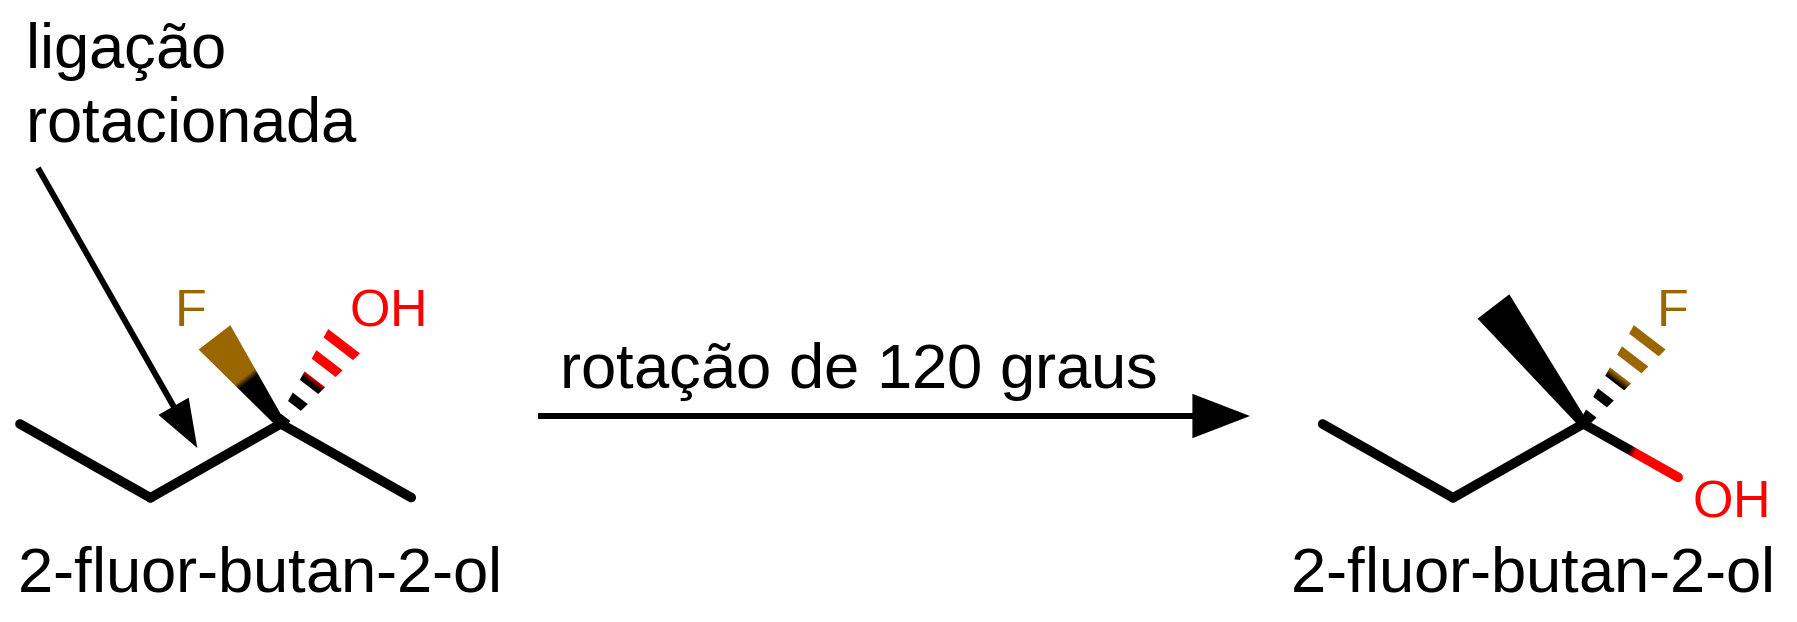
\includegraphics[width=0.75\linewidth]{imagens/rotacao.png}
\caption*{Fonte: Autores}
\end{figure}

A rotação aplicada à molécula representada à esquerda da Figura \ref{fig:rotacao} é completamente arbitrária, escolhida apernas para mostrar a liberdade rotacional presente na ligação Carbono-Carbono do tipo $\sigma$. Essa alteração rotacional ocorre muito rapidamente e modelos de dinâmica molecular podem ajudar os leitores mais curiosos \cite{Monticelli2013}. Porém, nem toda ligação sigma pode rotacionar livremente, pois ela pode fazer parte de uma cadeia cíclica ou estar associada a uma ligação $\pi$, formada pela \textbf{sobreposição lateral de orbitais puros}.

Inicialmente, considere o exemplo clássico do hidrocarboneto chamado \textbf{ciclo-hexano}, com estrutura exibida na Figura \ref{fig:ch}.

\begin{figure}[h]
\centering
\caption{Ciclo-hexano em modo bola/bastão, colorido.}
\vspace{0.25cm}
\label{fig:ch}
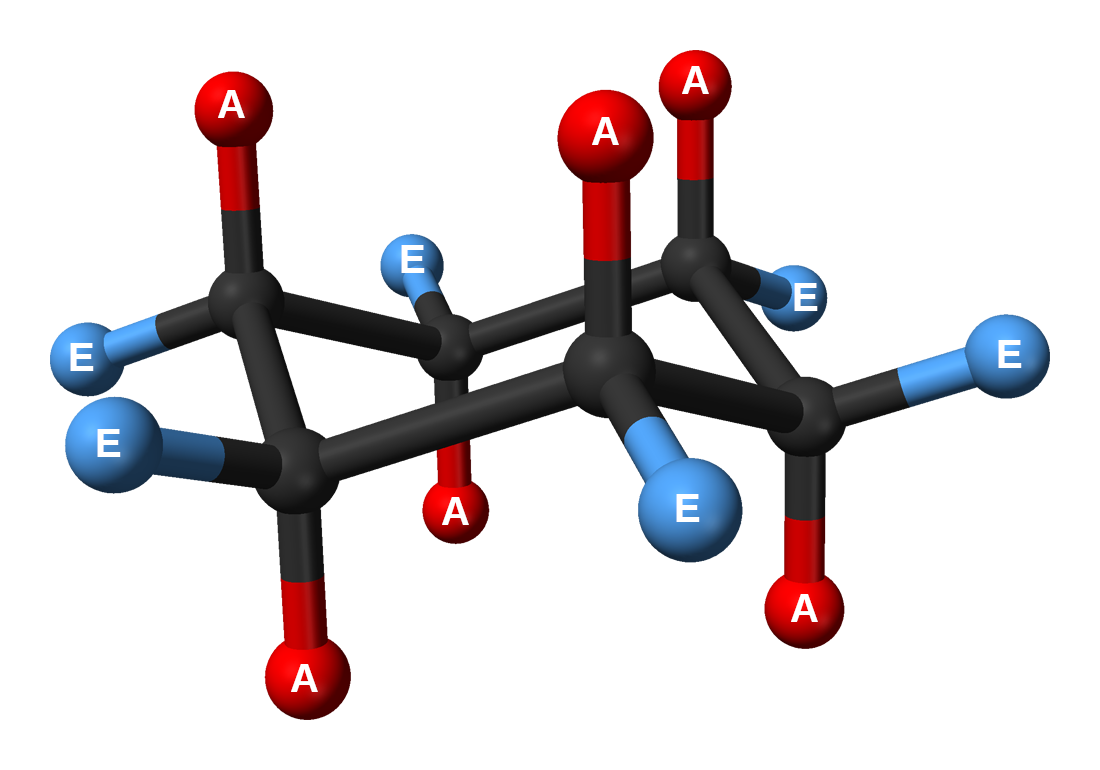
\includegraphics[width=0.6\linewidth]{imagens/Cyclohexane-chair-colour-coded-3D-balls.png}
\caption*{Fonte: Wikipedia, disponível em https://shorturl.at/fhEKU}
\end{figure}

A representação do ciclo-hexano na figura usa a notação \textbf{bola/bastão}, onde cada bastão representa uma ligação $\sigma$ (neste exemplo) e cada bola representa um átomo. Os átomos sem qualquer letra indicando símbolo são o átomos de carbono. A figura mostra dois tipos de átomos de hidrogênio nesta estrutura: aqueles marcados com a letra "A" e aqueles marcados com a letra "E". Neste exemplo, o código "A" indica os átomos de Hidrogênio em posição \textbf{axial} (considere um eixo vertical) enquanto o código "E" indica os áomos de Hidrogênio em posição \textbf{equatorial} (considere uma imaginária Linha do Equador, que divide o planeta Terra em hemisférios).

A limitada rotação possível de cada uma das ligações $\sigma$ nessa molécula causa apenas contorção e o ciclo-hexano assume diferentes \textbf{conformações}, que são arranjos espaciais provocados por rotação conjunta das ligações $\sigma$, mas limitadas em função da existência da cadeia cíclica \footnote{Não confunda \textbf{conformação} com \textbf{configuração}, pois esta última relaciona a topologia ou ordem a de conexão entre os átomos.}, conforme ilustra a figura \ref{fig:ch2}

\begin{figure}[h]
\centering
\caption{Análise conformacional do ciclo-hexano}
\vspace{0.25cm}
\label{fig:ch2}
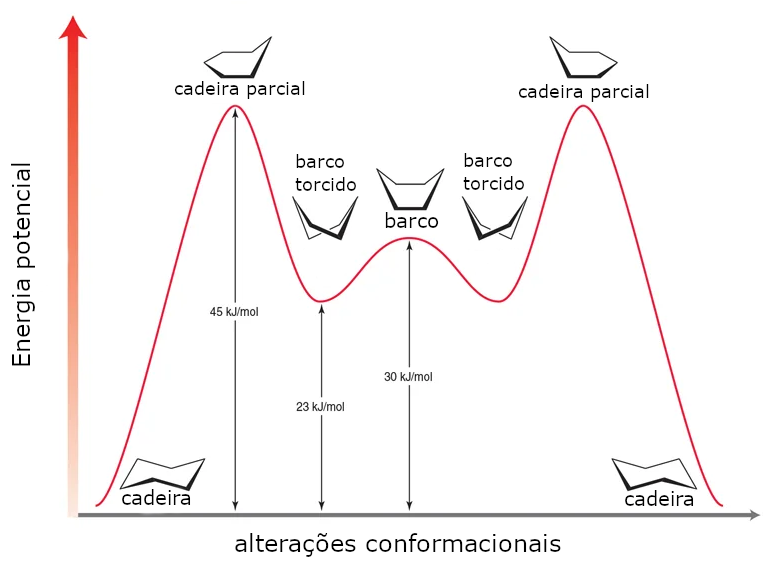
\includegraphics[width=0.85\linewidth]{imagens/analise_conformacional_ch_2.png}
\caption*{Fonte: Autores (checar origem da imagem)}
\end{figure}

A ideia central por trás dessas alterações conformacionais provocadas por rotação parcial das ligações sigma ($\sigma$) é \textbf{minimizar a repulsão eletrônica gerada por átomos de Hidrogênio}. Analisando a Figura \ref{fig:ch} podemos perceber que o ciclo-hexano em conformação \textbf{cadeira} possui energia potencial praticamente nula. Isso ocorre porque os átomos de Hidrogênio \textbf{axiais} e \textbf{equatoriais} estão distantes entre si o suficiente para eliminar uma eventual tensão angular ou torcional, estas provocadas por rotação parcial das ligações $\sigma$ entre átomos de Carbono.

A tensão que qualquer molécula pode apresentar corresponde a um excesso de energia provocado, por exemplo, por algum fator externo capaz de alterar seu estado de menor energia. Veja o caso da conformação \textbf{cadeira} do ciclo-hexano. A conformação \textbf{cadeira} possui esse nome porque existe uma certa senelhança entre a forma do ciclo-hexano nesta conformação quando comparada a uma cadeira. Você se acostuma com a ideia, acredite!

\begin{figure}[h]
\centering
\caption{Analogia da configuração cadeira do ciclo-hexano com uma cadeira.}
\vspace{0.25cm}
\label{fig:cadeira}
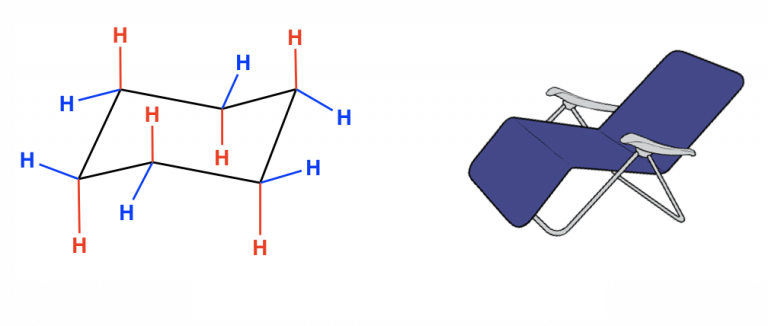
\includegraphics[width=0.75\linewidth]{imagens/chair-confirmation-analogue-768x326.png}
\caption*{Fonte: Kwantlen Polytechnic University (adaptada), disponível em https://shorturl.at/blT05}
\end{figure}

Energia fluindo do ambiente para as moléculas do ciclo-hexano a fazem vibrar e, consequentemente, torcer. Isso aumenta a repulsão entre os átomos de Hidrogênio, que era mínima, e sofre tensão torcional. Porém, um certo número de moléculas à temperatura ambiente possui energia suficiente para vibrar e, consequentemente, permitir a rotação parcial das ligações $\sigma$. Assim ocorrem as mudanças conformacionais, passando de \textbf{cadeira} para \textbf{cadeira parcial}, depois para \textbf{barco torcido}, passando para \textbf{barco}, novamente a \textbf{barco torcido} e finalmente retornando à conformação \textbf{cadeira}. A maior barreira energética para a interconversão conformacional do ciclo-hexano é de 45 kJ/mol, o que permite, à temperatura ambiente, perto de 10$^6$ conversões por segundo. Trataremos a análise conformacional em mais detalhes quando analisarmos hidrocarbonetos cíclicos.

\section{A ligação pi ($\pi$)}
Nosso cenário a respeito de ligaçãoes C-C fica um pouco mais complexo porque temos agora outro tipo de sobreposição de orbitais: a \textbf{sobreposição lateral}. Mas qual a razão deste novo tipo de sobreposição de orbitais? A frontal é insuficiente? Para compreender totalmente o novo modo de ligação que veremos a partir deste ponto, sugerimos que seja revista a Figura \ref{fig:hibridacao_traduzida}. Reproduzimos aqui uma parte da figura, destacando um ponto de grande importância na hibridização: a \textbf{combinação parcial de orbitais atômicos}.

\begin{figure}[h]
\centering
\caption{Exemplo da combinação parcial de orbitais atômicos}
\vspace{0.25cm}
\label{fig:}
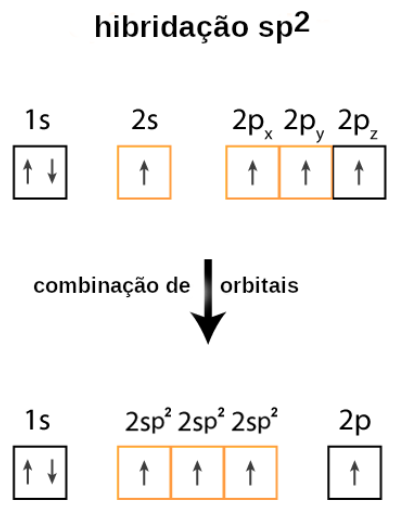
\includegraphics[width=0.45\linewidth]{imagens/sp2.png}
\caption*{Fonte: Autores}
\end{figure}

Quando o subnível 2s e o subnível 2p do átomo de Carbono tornam-se \textbf{degenerados} (igual conteúdo de energia), existem três possibilidades de combinação de orbitais puros para formar orbitais híbridos:

\begin{itemize}
	\item sp$^3$: combinação \textbf{total} entre os subníveis s e p;
	\item sp$^2$: combinação \textbf{parcial} entre os subníveis: 2s + 2 orbitais do subnível 2p;
	\item sp: combinação \textbf{parcial} entre os subníveis: 2s + 1 orbital 2p.
\end{itemize}

Nosso foco está nas combinações \textbf{parciais}, nas quais um ou dois orbitais p puros do subnível 2p não participaram do processo de combinação. Conforme podemos observar na Figura \ref{fig:vistas_sp2}, quando a combinação de orbitais envolve apenas dois dos três orbitais do subnível p, forma-se um subnível híbrido  \textbf{sp$^2$}, contendo três orbitais e um orbital p permanece intacto. Aqui está o ponto central: os três orbitais híbridos sp$^2$ são \textbf{coplanares} e o orbital p puro está em posição \textbf{ortogonal} em relação aos híbridos sp$^2$. Assim, quando dois orbitais sp$^2$ sobrepõem-se de modo frontal, formando uma ligação sigma, dois orbitais p puros ficam paralelos entre si, possibilitando a \textbf{sobreposição lateral}.

\begin{figure}[h]
\centering
\caption{Vistas lateral e superior do subnível sp$^2$}
\vspace{0.25cm}
\label{fig:vistas_sp2}
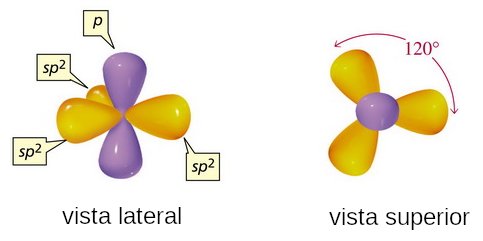
\includegraphics[width=0.65\linewidth]{imagens/hibrido_sp2.png}
\caption*{Fonte: Autores (checar a origem)}
\end{figure}

Embora a sobreposição lateral também seja uma ligação química, sua formação e propriedades são bem distintas daquela da ligação sigma, e possibilita a ocorrência de, por exemplo, duas entidades de crucial importância em Química Orgânica: \textbf{conjugação} e \textbf{ressonância}. A Figura \ref{fig:sobre_lateral} ilustra o processo de formação da ligação pi ($\pi$) por meio da sobreposição lateral de orbitais puros.

\begin{figure}[h]
\centering
\caption{Sobreposição lateral e formação da ligação $\pi$}
\vspace{0.25cm}
\label{fig:sobre_lateral}
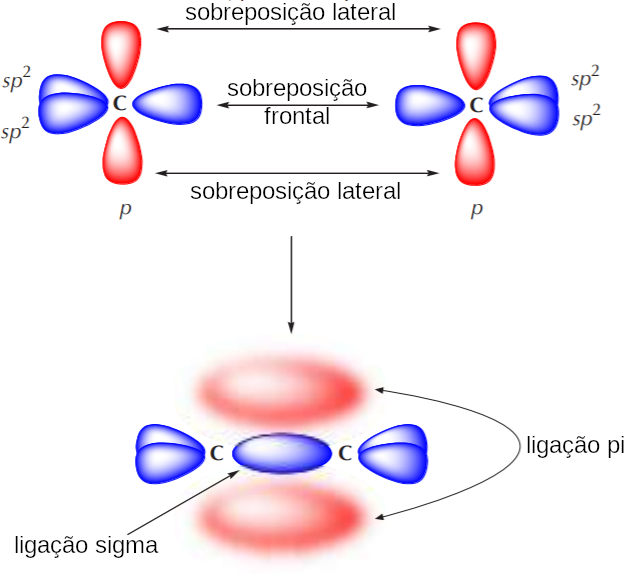
\includegraphics[width=0.75\linewidth]{imagens/sobre_lateral.png}
\caption*{Fonte: LibreTexts Chemistry (adaptada), disponível em https://shorturl.at/jnKU1}
\end{figure}

Analisando a figura \ref{fig:sobre_lateral}, percebemos o mecanismo de formação da ligação $\pi$ com a aproximação horizontal dos dois átomos de Carbono que se ligarão. Na parte superior da figura, dois orbitais híbridos se aproximam de modo horizontal e ocorrerá a sobreposição \textbf{frontal} destes orbitais, formando a ligação sigma. Porém, aproximando os dos dois átomos de Carbono também aproximam-se dois orbitais \textbf{p} puros o suficiente para que ocorra a \textbf{sobreposição lateral} destes orbitais.

Como o orbital p puro é formado por dois lobos, um acima e outro abaixo do plano nodal (aquele que passa pelo núcleo do átomo), existem duas regiões de sobreposição, uma acima e outra abaixo da ligação $\sigma$. Considerando que orbitais estão diretamente relacionados com probabilidade de encontrar um elétron, de forma muito simplificada, podemos encontrar o par eletrônico da ligação $\pi$ \textbf{acima} ou \textbf{abaixo} da ligação $\sigma$, o que justifica as duas regiões presentes na parte de baixo da Figura \ref{fig:sobre_lateral}.

Existem outras possibilidades de combinação entre os orbitais, como por exemplo aquela que envolve um orbital puro \textbf{s} e um orbital puro \textbf{p}, formando um conjunto de orbitais híbridos chamado de \textbf{sp}, característicos de ligações carbono-carbono do tipo tripla (\ce{-C#C-}) ou então de sistemas \textbf{alênicos}, onde temos três átomos de carbono ligados por \textbf{duas} ligações duplas (\ce{C=C=C}).

No caso da ligação carbono-carbono do tipo tripla, os dois átomos de carbono apresentam hibridização sp e geometria linear, assim como o carbono central do sistema alênico, o que confere algumas características químicas partculares a sistemas como os descritos, conforma pode ser visto na figura \ref{fig:tripla}.

\begin{figure}[h]
\centering
\caption{Carbonos com hibridização sp: a ligação tripla}
\vspace{0.25cm}
\label{fig:tripla}
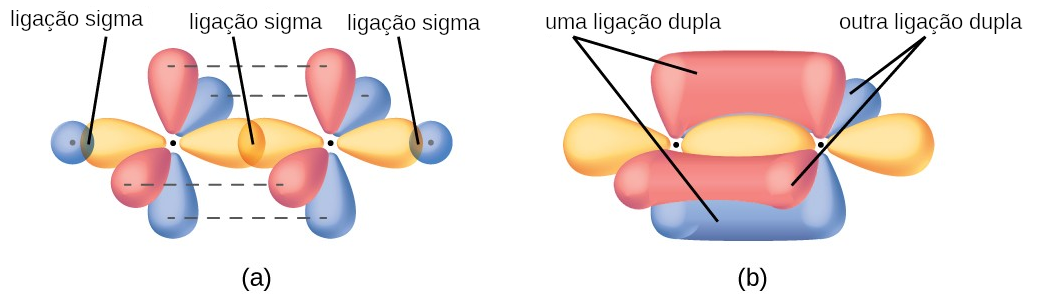
\includegraphics[width=1\linewidth]{imagens/tripla.png}
\caption*{Fonte: LibreTexts, adaptada, disponível em https://shorturl.at/hikBG}
\end{figure}

Analisando a parte (a) da figura \ref{fig:tripla}, percebemos a sobreposição frontal de orbitais puros ou híbridos (ligação $\sigma$) e também um tracejado que indica a sobreposição lateral de orbitais p puros (ligação $\pi$). Ao analisarmos a parte (b) da mesma figura, identificamos, com cores diferentes, as duas ligações duplas formadas entre dois átomos de carbono com hibridização sp. 

\chapter{Introdução às funções orgânicas}
\begin{mdframed}[backgroundcolor=orange!20,linewidth=0pt,roundcorner=10pt]
	\minitoc
\end{mdframed}
As funções orgânicas são grupos de compostos químicos que compartilham características estruturais e propriedades químicas semelhantes. Elas desempenham um papel fundamental na Química Orgânica, que é o ramo da Química que se concentra no estudo dos compostos que contêm carbono. Os compostos orgânicos podem ser encontrados em uma variedade impressionante de formas e tamanhos, e as funções orgânicas são a maneira pela qual os químicos classificam e compreendem essa diversidade.

As funções orgânicas são essenciais para entender a química dos compostos orgânicos e desempenham um papel crucial em muitos aspectos da química, incluindo a síntese de produtos químicos, a bioquímica, a farmacologia e a indústria química. Esta introdução pretende explorar algumas das funções orgânicas mais comuns e destacará sua importância no estudo da Química Orgânica e na vida cotidiana.


\section{Reconhecimento de padrões}
Faça um exercício mental simples: você consegue separar os bilhões de seres humanos que habitam o planetinha azul chamado Terra de acordo com alguma característica? Analisando friamente, percebemos diferenças no formato dos olhos, na pigmentação da pele, no formato dos cabelos, entre tantas outras características. Se você agrupou alguns humanos, você provavelmente chegou perto de uma etnia. Paramos por aqui com humanos.

Igualmente, se você decidir agrupar automóveis segundo, por exemplo, a potência do motor, número de portas ou qualquer outra característica, você criou uma categoria automobilística.

Este exercício pode ser repetido com músicas, livros, filmes computadores, celulares, ou números, entre tantos outros possíveis elementos que podem ser agrupados.

Fácil, certo?

Sim, desde que você defina alguma característica que diferencie um grupo de outro e coloque junto entidades com características semelhantes.

Antes de tratarmos de moléculas orgânicas, você precisa acostumar seu cérebro naquilo que é conhecido como \textbf{"Reconhecimento de Padrões"}. Veja como nem sempre é simples. oi

\begin{table}[!h]
	\begin{center}
	\caption{\label{padroes}Exercício simples sobre reconhecimento de padrões}
	\vspace{0.5cm}
	\begin{tabular}{|c | c | c|}
	\hline
	4 & 15 & 5\\
	\hline
	5 & 24 & 8\\
    \hline
	2 & 3 & 1\\
	\hline
    7 & \textbf{x} & 16\\
    \hline
	\end{tabular}
	\end{center}
\end{table}

Como você encontra o valor desconhecido apresentado na tabela \ref{padroes}? Existe um padrão que se repete em todas as linhas e caso o encontre nas três primeiras linhas, o valor de x quase que emerge de seu cérebro. 

Quanto tempo levou para encontrar o padrão, principalmente até se dar conta de que pode ignorar a coluna numérica da esquerda?

Independente do tempo gasto na resolução do problema, o padrão escondido nos números é bem simples: os valores numéricos da coluna central são \textbf{o triplo} dos valores da coluna numérica da direita. Assim, o valor de x deve ser o triplo de 16, ou seja, 48.

Existe um outro aspecto que deve ser considerado neste ponto de nossa análise sobre funções orgânicas: a similaridade. De modo bem simplificado, podemos admitir que similaridade está muito relacionada com semelhança e assim podemos dizer que a entidade A é similar à entidade B se vários elementos presentes em A também estejam presentes na entidade B.

Considere a Figura \ref{fig:carros} a seguir. Nela podemos visualizar um conjunto de desenhos com a parte dianteira de alguns automóveis fictícios.

\begin{figure}[h]
	\centering
	\caption{Representação de alguns automóveis.}
	\vspace{0.5cm}
	
\includegraphics[width=0.5\linewidth]{imagens/19035-NRYBNX.jpg}
    \caption*{Fonte: https://shorturl.at/crzG0}
	\label{fig:carros}
\end{figure}

A Figura \ref{fig:carros} neste contexto ajuda a praticar a busca por similaridade em imagens, algo que será muito útil quando precisarmos identificar todas as funções orgânicas presentes em uma molécula polifuncional, pois uma destas funções deve ser a chamada "sênior" ou "principal" para que possamos montar o seu nome a partir de sua estrutura.

Quais elementos tornam as seis partes da imagem representada na figura similares entre si? Podemos visualizar alguns elementos presentes em todas as imagens:

\begin{itemize}
	\item Duas rodas visíveis.
	\item Dois espelhos retrovisores
	\item Um para-brisa
\end{itemize}

Repare que os faróis dos automóveis não são idênticos, assim como as grades frontais também são distintas. Assim, as representações dos automóveis são similares em algum aspecto.

%########################
\section{Função orgânica}
O mesmo ocorrerá quando precisarmos analisar uma estrutura orgânica complexa em busca das funções orgânicas presentes. Veja a molécula representada na Figura \ref{fig:vanco} a seguir.

\begin{figure}[h]
	\centering
	\caption{Estrutura da vancomicina}
	\vspace{0.5cm}
	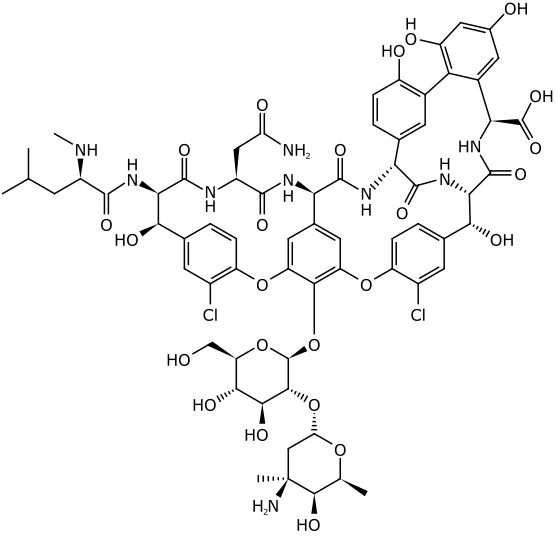
\includegraphics[width=0.85\linewidth]{imagens/557px-Vancomycin.svg}
	\caption*{Fonte: Wikipedia https://shorturl.at/nAZ01}
	\label{fig:vanco}
\end{figure}

Ainda sem analisar os detalhes de cada função orgânica presente na vancomicina, uma substância classificada como antibiótico, percebe-se que existem alguns conjuntos de átomos que se repetem na estrutura, algo como (guardadas as devidas proporções) ocorre na Figura \ref{fig:carros}.

É relativamente fácil encontrar alguns desses grupos de átomos:

\begin{itemize}
	\item átomo de Oxigênio ligado a átomo de Hidrogênio;
	\item átomo de Nitrogênio ligado a dois átomos de Oxigênio;
	\item átomo de Carbono ligado a um átomo de Oxigênio por uma ligação covalente dupla.
\end{itemize}

Cada um desses conjuntos é uma \textbf{função orgânica}.

Existem dezenas delas, todas categorizadas, organizadas e designadas por seus nomes pela IUPAC, conforme pode ser analisado no IUPAC BlueBook \cite{iupac2013}.

O número de substâncias orgânicas conhecidas já ultrapassou a grandeza de dezenas de milhões, e métodos sintéticos novos geram ainda mais substâncias \cite{doi:10.1021/acs.jmedchem.2c00223}. Cada substância química precisa de um nome que caracterize sua unicidade e existem muitas regras para que cada uma delas tenha seu nome de maneira inequívoca.

A Figura \ref{fig:funcoes2} mostra um resumo das funções orgânicas que serão analisadas neste livro, contendo, além do nome, uma representação geral e também o sufixo correspondente.

\begin{figure}[h]
	\centering
	\caption{Resumo das funções orgânicas.}
	\vspace{0.5cm}
	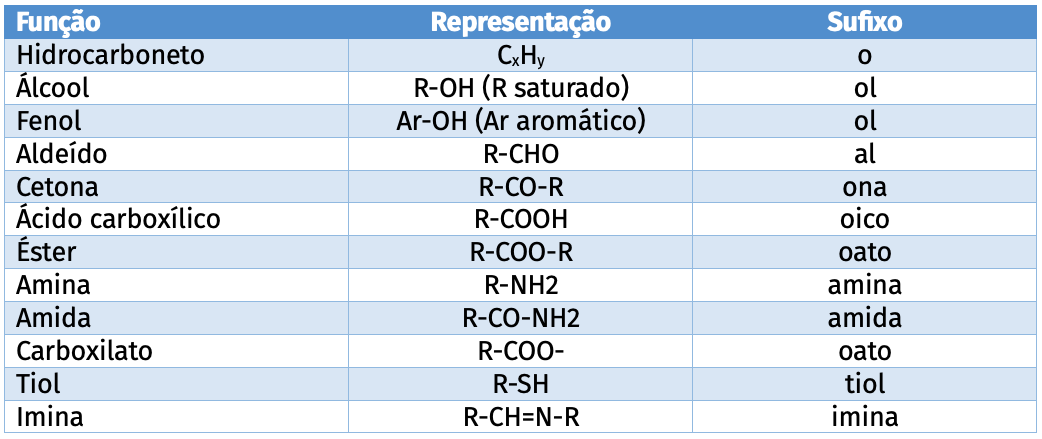
\includegraphics[width=1\linewidth]{imagens/funcoes.png}
	\caption*{Fonte: autores}
	\label{fig:funcoes2}
\end{figure}

%###################################


\chapter{Hidrocarbonetos}
\begin{mdframed}[backgroundcolor=orange!20,linewidth=0pt,roundcorner=10pt]
	\minitoc
\end{mdframed}
Os hidrocarbonetos são uma classe fundamental de compostos químicos que desempenham um papel central na química orgânica. Eles consistem exclusivamente em átomos de carbono e hidrogênio, formando uma família diversificada de moléculas que variam desde as mais simples até as mais complexas. A simplicidade de sua composição, que consiste apenas em dois elementos, torna os hidrocarbonetos um dos grupos de compostos mais estudados e essenciais na química orgânica, e um exemplo destes pode ser visto na figura \ref{fig:ocatene}

\begin{figure}[h]\centering
\caption{Um hidrocarboneto encontrado no petróleo}
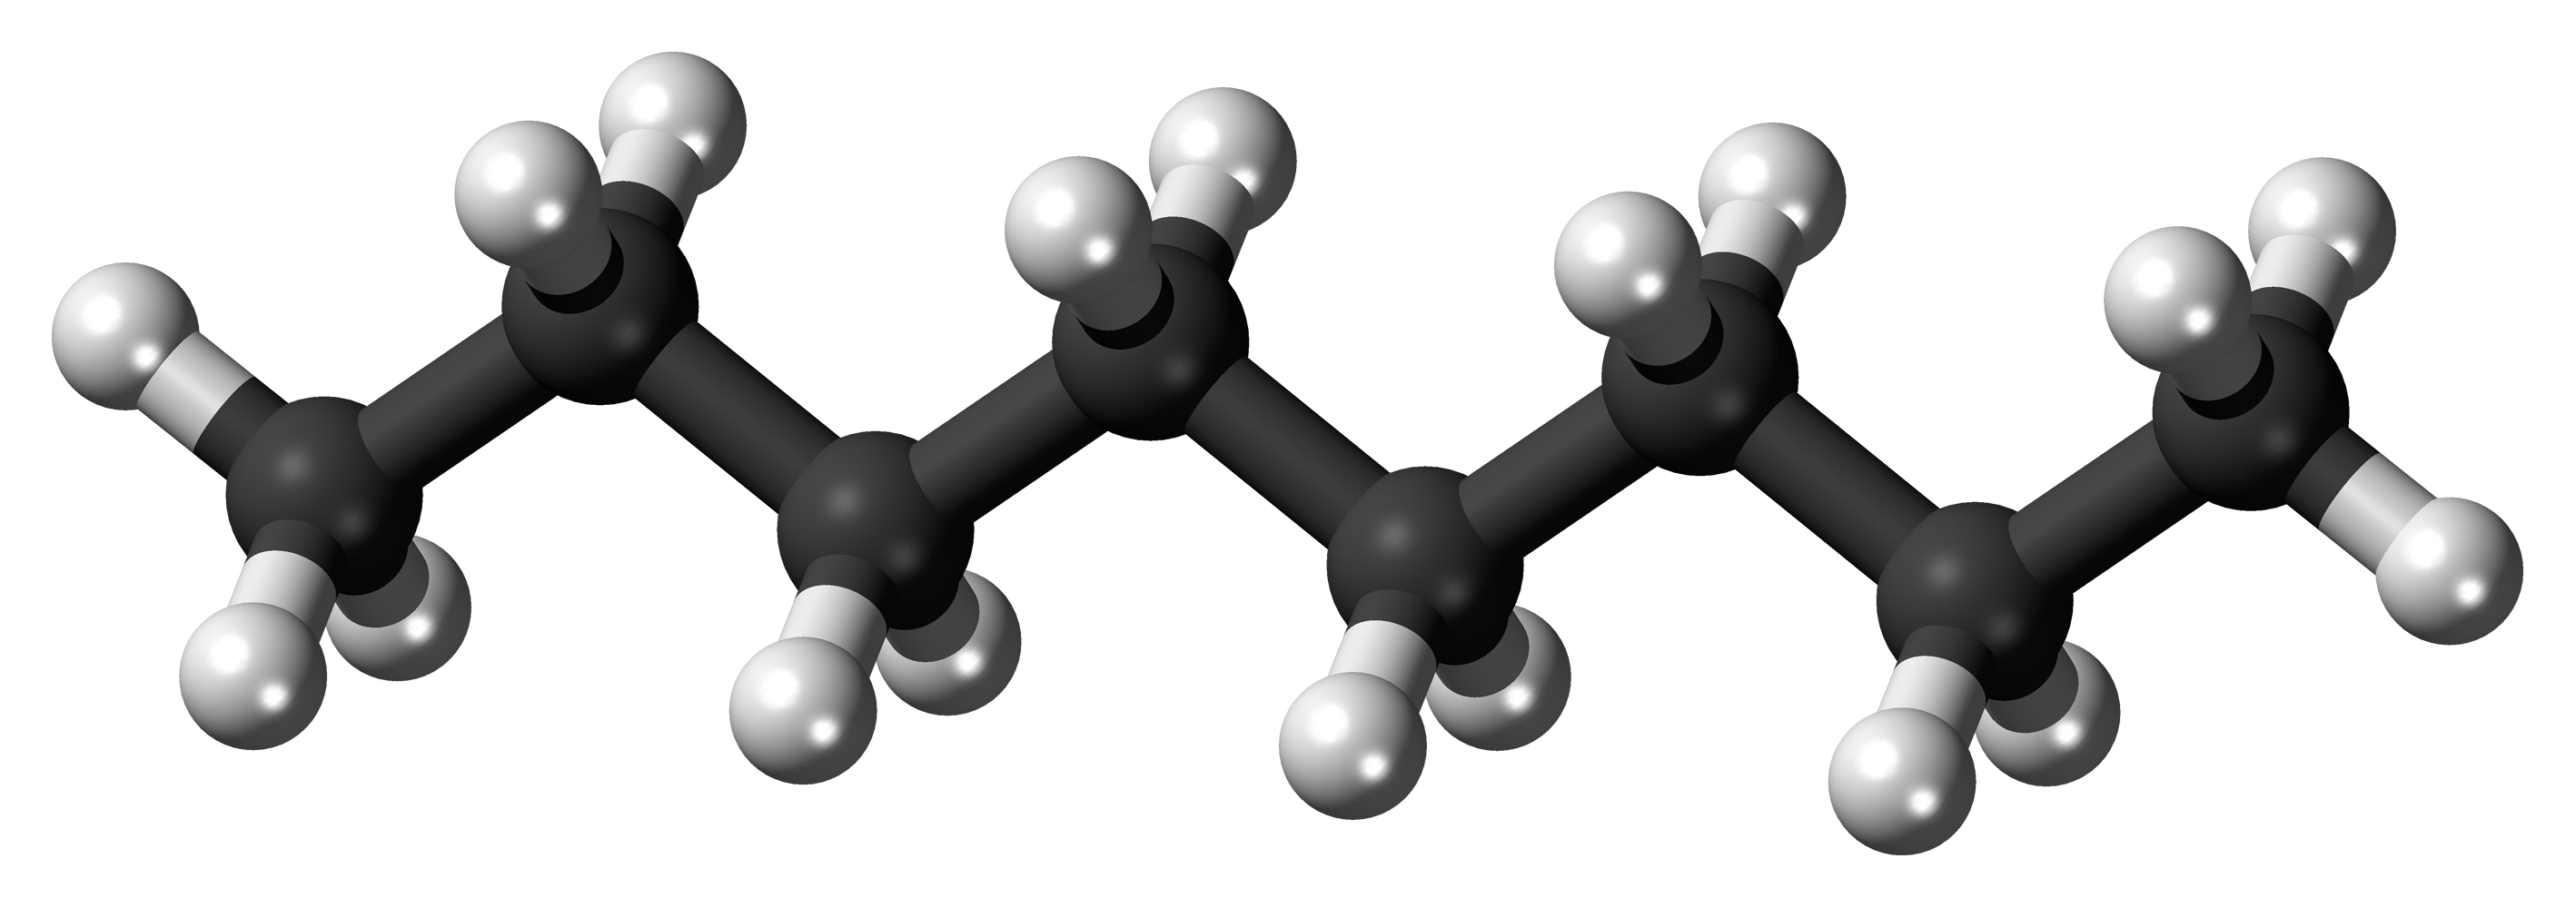
\includegraphics[scale=0.175]{imagens/Octane_3D_ball.png}
\label{fig:ocatene}\vspace{0.5cm}\end{figure}

Algumas das características da representação estrutural presente na figura \ref{fig:ocatene} serão úteis em diversos outros momentos deste livro e podemos tratar rapidamente sobre algumas delas. Repare que a figura apresenta tubos (para representar ligações covalentes) e esferas (para representar átomos). Os átomos mais claros são Hidrogênio e os mais escuros são Carbono. Um único tubo entre dois átomos representa uma \textbf{ligação covalente simples}, dois tubos representam uma \textbf{ligação covalente dupla} (ausente na figura) e três tubos representam a \textbf{ligação covalente tripla} (também ausente na figura).

Ainda na figura \ref{fig:ocatene}, todos os átomos de carbono encontram-se ligados por ligações covalentes simples, o que classifica essa sequência de átomos de carbono, a partir deste ponto chamada de \textbf{cadeia carbônica} como \textbf{cadeia saturada}. Caso a cadeia carbônica possua uma ligação covalente dupla entre o carbono da extremidade esquerda e seu vizinho imediato (neste exemplo), conforme pode ser visto na figura \ref{fig:hexene}, a cadeia passa a ser classificada como insaturada.

\begin{figure}[h]\centering
\caption{Um hidrocarboneto insaturado}
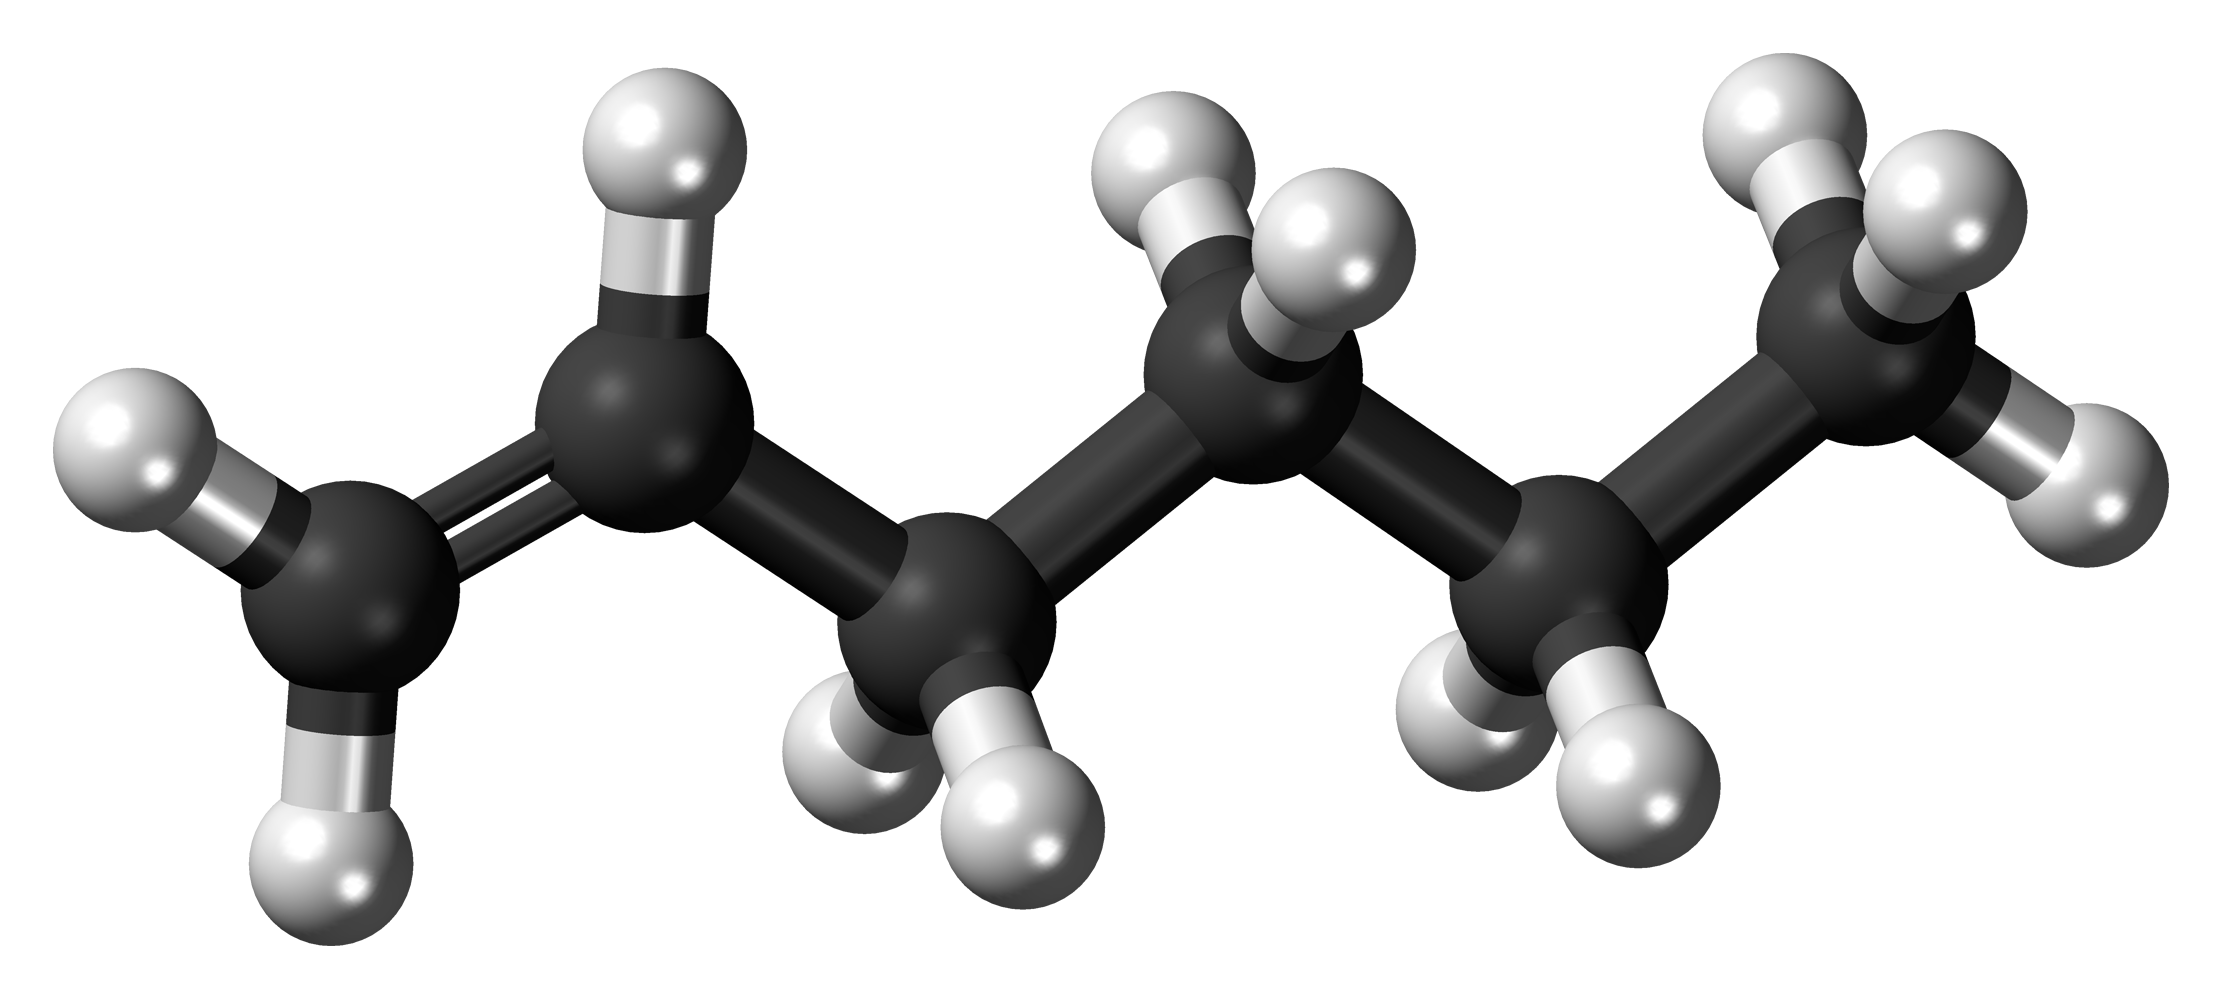
\includegraphics[scale=0.225]{imagens/1-Hexene-3D-balls.png}
\label{fig:hexene}\vspace{0.5cm}\end{figure}

Os hidrocarbonetos desempenham um papel vital em inúmeros aspectos da nossa vida cotidiana. Eles são os principais constituintes dos combustíveis fósseis, como petróleo e gás natural, que propulsionam nossos veículos e fornecem energia para a geração de eletricidade. Além disso, muitos produtos químicos, plásticos e materiais sintéticos são derivados de hidrocarbonetos.

Esta introdução explorará a estrutura básica dos hidrocarbonetos, suas diferentes categorias e sua relevância em várias aplicações, desde o setor energético até a indústria química e farmacêutica, destacando sua importância na química orgânica e na nossa sociedade moderna.
\section{Origens do petróleo}
A teoria orgânica para a origem do petróleo é uma das explicações mais aceitas para a formação desse recurso natural. Ela postula que o petróleo se origina a partir da decomposição de matéria orgânica, como plantas e microorganismos, ao longo de milhões de anos sob condições específicas de pressão e temperatura no subsolo. Esta teoria foi proposta pela primeira vez no século XIX e é conhecida como a teoria biogênica.

A \textbf{teoria orgânica} descreve o processo de formação do petróleo da seguinte maneira:

1. Acúmulo de Matéria Orgânica: No passado geológico, oceanos e lagos continham uma grande quantidade de matéria orgânica em diferetnes estados de decomposição, incluindo plâncton, algas e outros resíduos biológicos. Toda essa matéria orgânica se acumulava no fundo dessas águas, onde a falta de oxigênio limitava a decomposição completa.

2. Sepultamento: Com o tempo, sedimentos foram se acumulando sobre a matéria orgânica, causando seu sepultamento no subsolo. Essa incrível sobreposição de sedimentos exerceu pressão sobre a matéria orgânica, comprimindo-a.

3. Aumento de Temperatura e Pressão: À medida que os sedimentos continuaram a se acumular, a temperatura e a pressão no subsolo aumentaram gradualmente. A essa profundidade, a matéria orgânica passou por uma série de transformações químicas conhecidas como diagênese. Durante esse processo, a matéria orgânica se transformou em uma mistura complexa de hidrocarbonetos.

4. Migração e Armazenamento: Os hidrocarbonetos resultantes do processo de diagênese migraram através de rochas porosas e segmentos impermeáveis em direção às camadas superiores. Eles eventualmente ficaram presos em bolsas subterrâneas, formando reservatórios de petróleo.

5. Processo de Maturação: Com o tempo, os hidrocarbonetos continuaram a sofrer mudanças químicas, refinando-se e produzindo petróleo bruto, gás natural e outros componentes. A qualidade e a composição do petróleo podem variar dependendo das condições geológicas locais.

É importante observar que a teoria orgânica não é a única explicação para a origem do petróleo. Existem outras teorias, como a teoria abiótica, que sugere que o petróleo pode ser formado a partir de processos químicos não relacionados à matéria orgânica. No entanto, a teoria orgânica é amplamente aceita e tem uma base sólida na geologia e na química orgânica. Ela também se alinha com a grande quantidade de evidências geológicas e experimentais coletadas ao longo de muitas décadas.

A teoria inorgânica para a origem do petróleo é uma explicação alternativa à teoria orgânica predominante. Enquanto a teoria orgânica postula que o petróleo se forma a partir da decomposição de matéria orgânica, como microorganismos marinhos e plantas terrestres, a teoria inorgânica sugere que o petróleo pode se originar de processos não relacionados a organismos vivos.

A \textbf{teoria inorgânica} propõe que o petróleo é formado por reações químicas no interior da Terra, envolvendo elementos inorgânicos, como carbono, hidrogênio e nitrogênio. Os defensores dessa teoria argumentam que o petróleo é encontrado em profundidades muito maiores do que seria esperado se fosse proveniente de restos orgânicos, e que os processos geológicos e químicos subterrâneos podem produzir hidrocarbonetos a partir de substâncias não orgânicas.

Uma das principais hipóteses dentro da teoria inorgânica é a abiotica, que sugere que o petróleo é produzido por reações químicas de alta pressão e temperatura no manto da Terra, muito abaixo da camada onde a matéria orgânica é encontrada. Essas reações envolvem a transformação de minerais ricos em carbono, como calcário e magnésio, em hidrocarbonetos.

No entanto, é importante destacar que a teoria inorgânica enfrenta desafios significativos e não é amplamente aceita na comunidade científica. A teoria orgânica tem uma base sólida de evidências geológicas, juntamente com evidências geoquímicas e paleontológicas que apoiam a origem orgânica do petróleo. Além disso, a teoria inorgânica ainda não conseguiu explicar completamente a diversidade de compostos encontrados no petróleo cru.

\section{Classificação}
A classificação de hidrocarbonetos é um tópico fundamental na química orgânica, uma vez que os hidrocarbonetos constituem a base de muitos compostos orgânicos. Os hidrocarbonetos são compostos formados exclusivamente por átomos de carbono (C) e hidrogênio (H) e podem ser categorizados de acordo com a natureza das ligações entre os átomos de carbono e sua estrutura geral. Existem três grandes  categorias principais de hidrocarbonetos: alcanos, alcenos e alcinos, cada uma com características distintas.

1. \textbf{Alcanos}: são hidrocarbonetos que possuem apenas em ligações simples (ligações sigma) entre os átomos de carbono. Eles são conhecidos como hidrocarbonetos saturados, pois apresentam a máxima quantidade possível de hidrogênios. A fórmula geral dos alcanos é CnH2n+2, onde "n" representa o número de átomos de carbono na cadeia. Exemplos de alcanos incluem o metano (\ce{CH4}), o etano (\ce{C2H6}), o propano (\ce{C3H8}) e o butano (\ce{C4H10}). Alcanos têm pontos de ebulição mais baixos e são geralmente menos reativos em comparação com outras classes de hidrocarbonetos.

\begin{figure}[h]\centering
\caption{Um exemplo de hidrocarboneto do tipo alcano, com fórmula molecular \ce{C8H18}}
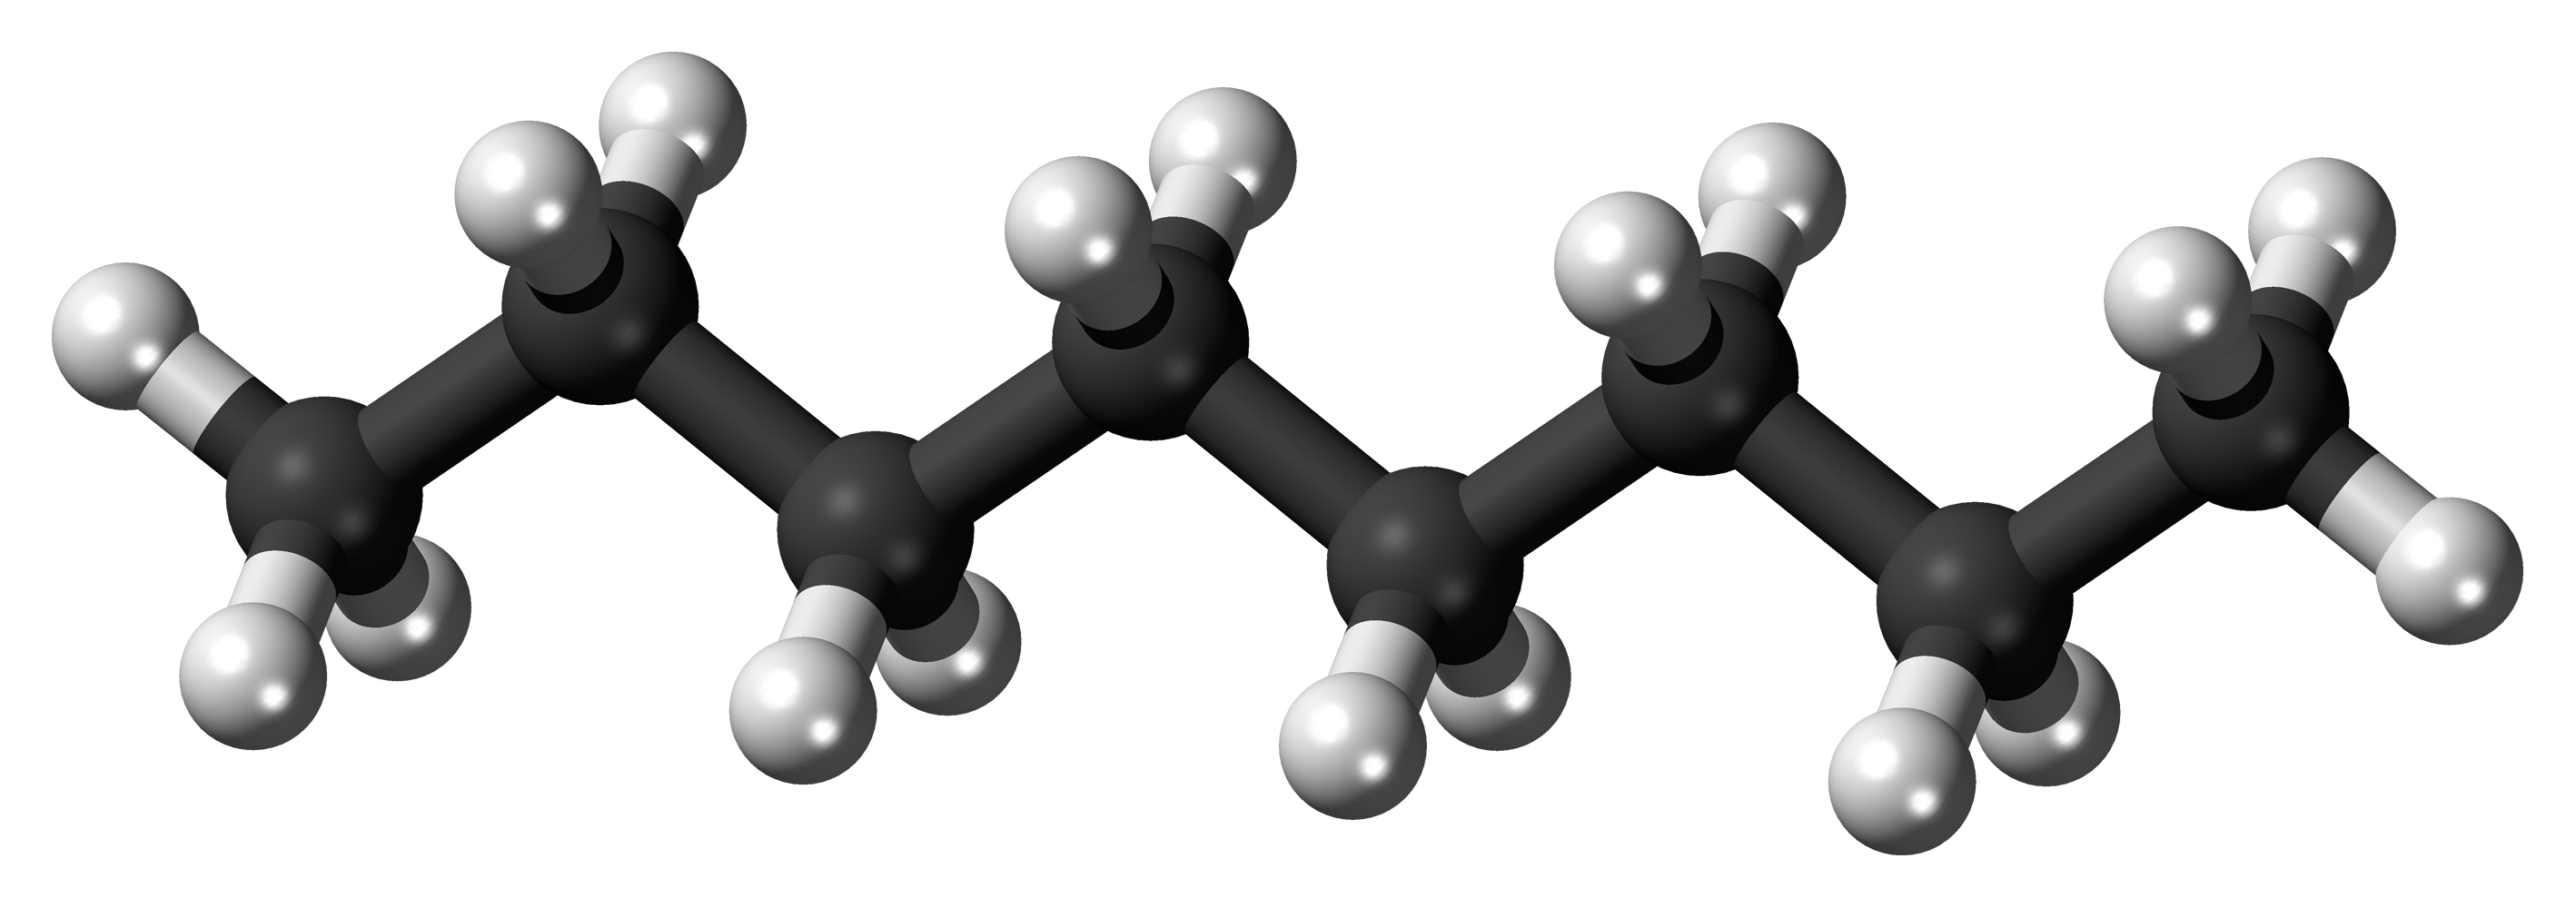
\includegraphics[scale=0.15]{imagens/Octane_3D_ball.png}
\label{fig:alcano}\vspace{0.5cm}\end{figure}

2. \textbf{Alcenos}:
Os alcenos são hidrocarbonetos que contêm pelo menos uma ligação dupla (ligação pi) entre átomos de carbono na cadeia. A fórmula geral dos alcenos é CnH2n, onde "n" representa o número de átomos de carbono na cadeia. A presença da ligação dupla introduz uma insaturação na molécula. Exemplos de alcenos incluem o eteno (\ce{C2H4}), o propeno (\ce{C3H6}) e o buteno (\ce{C4H8}). Os alcenos tendem a ser mais reativos do que os alcanos devido à presença da ligação dupla, que permite a ocorrência de reações de adição.

3. \textbf{Alcinos}:
Os alcinos são hidrocarbonetos que contêm pelo menos uma ligação tripla (duas ligações pi e uma ligação sigma) entre átomos de carbono na cadeia. A fórmula geral dos alcinos é CnH2n-2, onde "n" representa o número de átomos de carbono na cadeia. A ligação tripla torna os alcinos ainda mais reativos do que os alcenos e alcanos. Exemplos de alcinos incluem o etino (C2H2) e o propino (C3H4). Devido à sua alta reatividade, os alcinos são frequentemente usados como intermediários em sínteses orgânicas.

Além dessa classificação básica, os hidrocarbonetos também podem ser classificados com base na sua estrutura ramificada ou cíclica:

1. \textbf{Ramificados}:

Hidrocarbonetos podem apresentar grupos alquilas, também ligados à cadeia principal. A presença de destas leva à formação de isômeros, que são compostos com a mesma fórmula molecular, mas com diferentes arranjos espaciais. Os isômeros podem ter propriedades químicas e físicas distintas.

\begin{figure}[h]\centering
\caption{Um exemplo de hidrocarboneto ramificado}
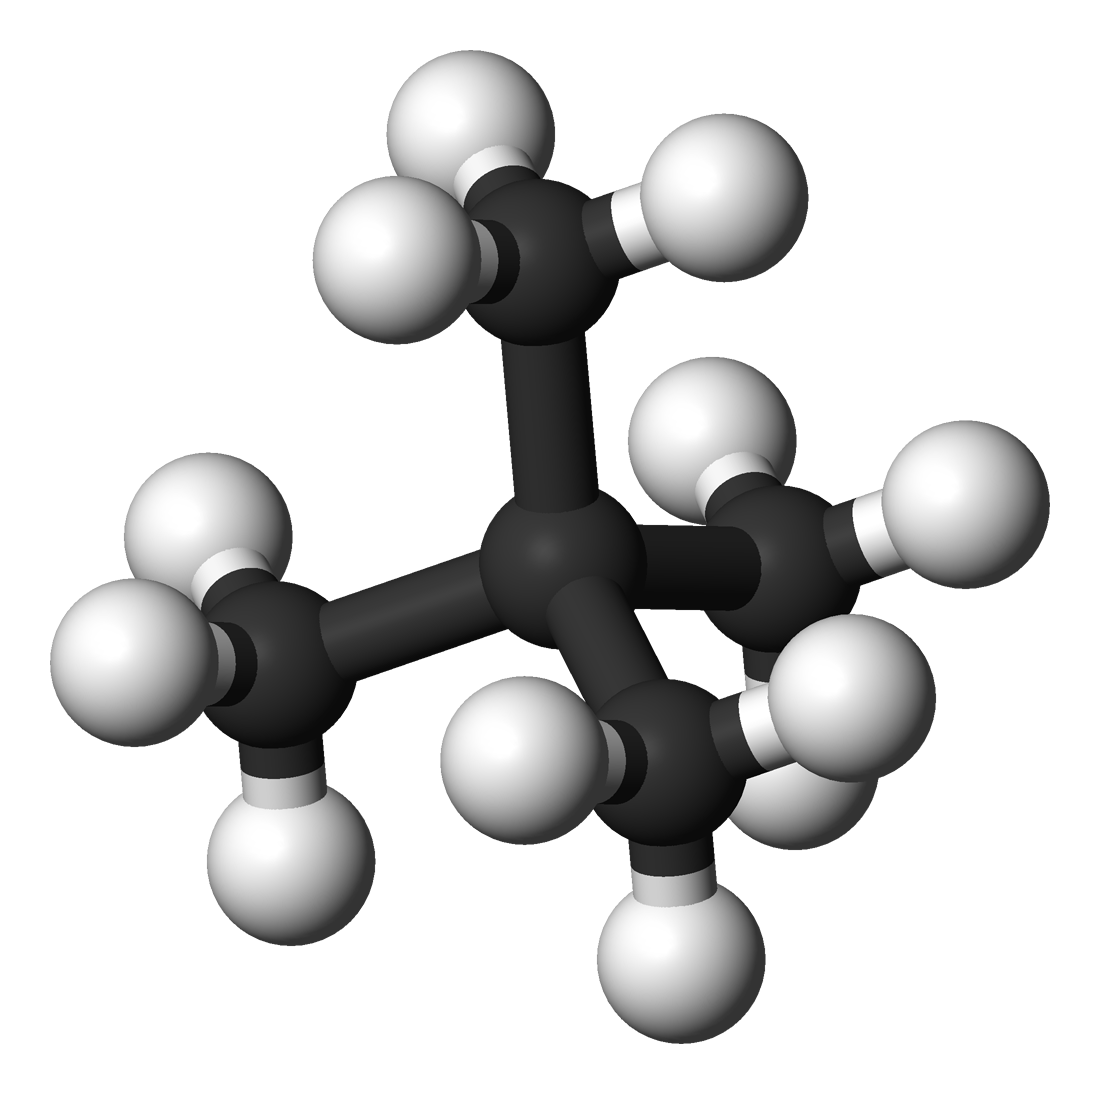
\includegraphics[scale=0.125]{imagens/Neopentane-3D-balls.png}
\label{fig:ramificado}\vspace{0.5cm}\end{figure}

2. \textbf{Cíclicos}:

Muitos hidrocarbonetos formam anéis fechados em suas estruturas. Esses compostos são chamados de hidrocarbonetos cíclicos. O ciclo mais simples é o ciclopropano, composto por um anel de três carbonos. Cicloexano, ciclopentano e ciclobutano são outros exemplos de hidrocarbonetos cíclicos.

\begin{figure}[h]\centering
\caption{Representação do cicloexano na notação \textbf{bastão}}
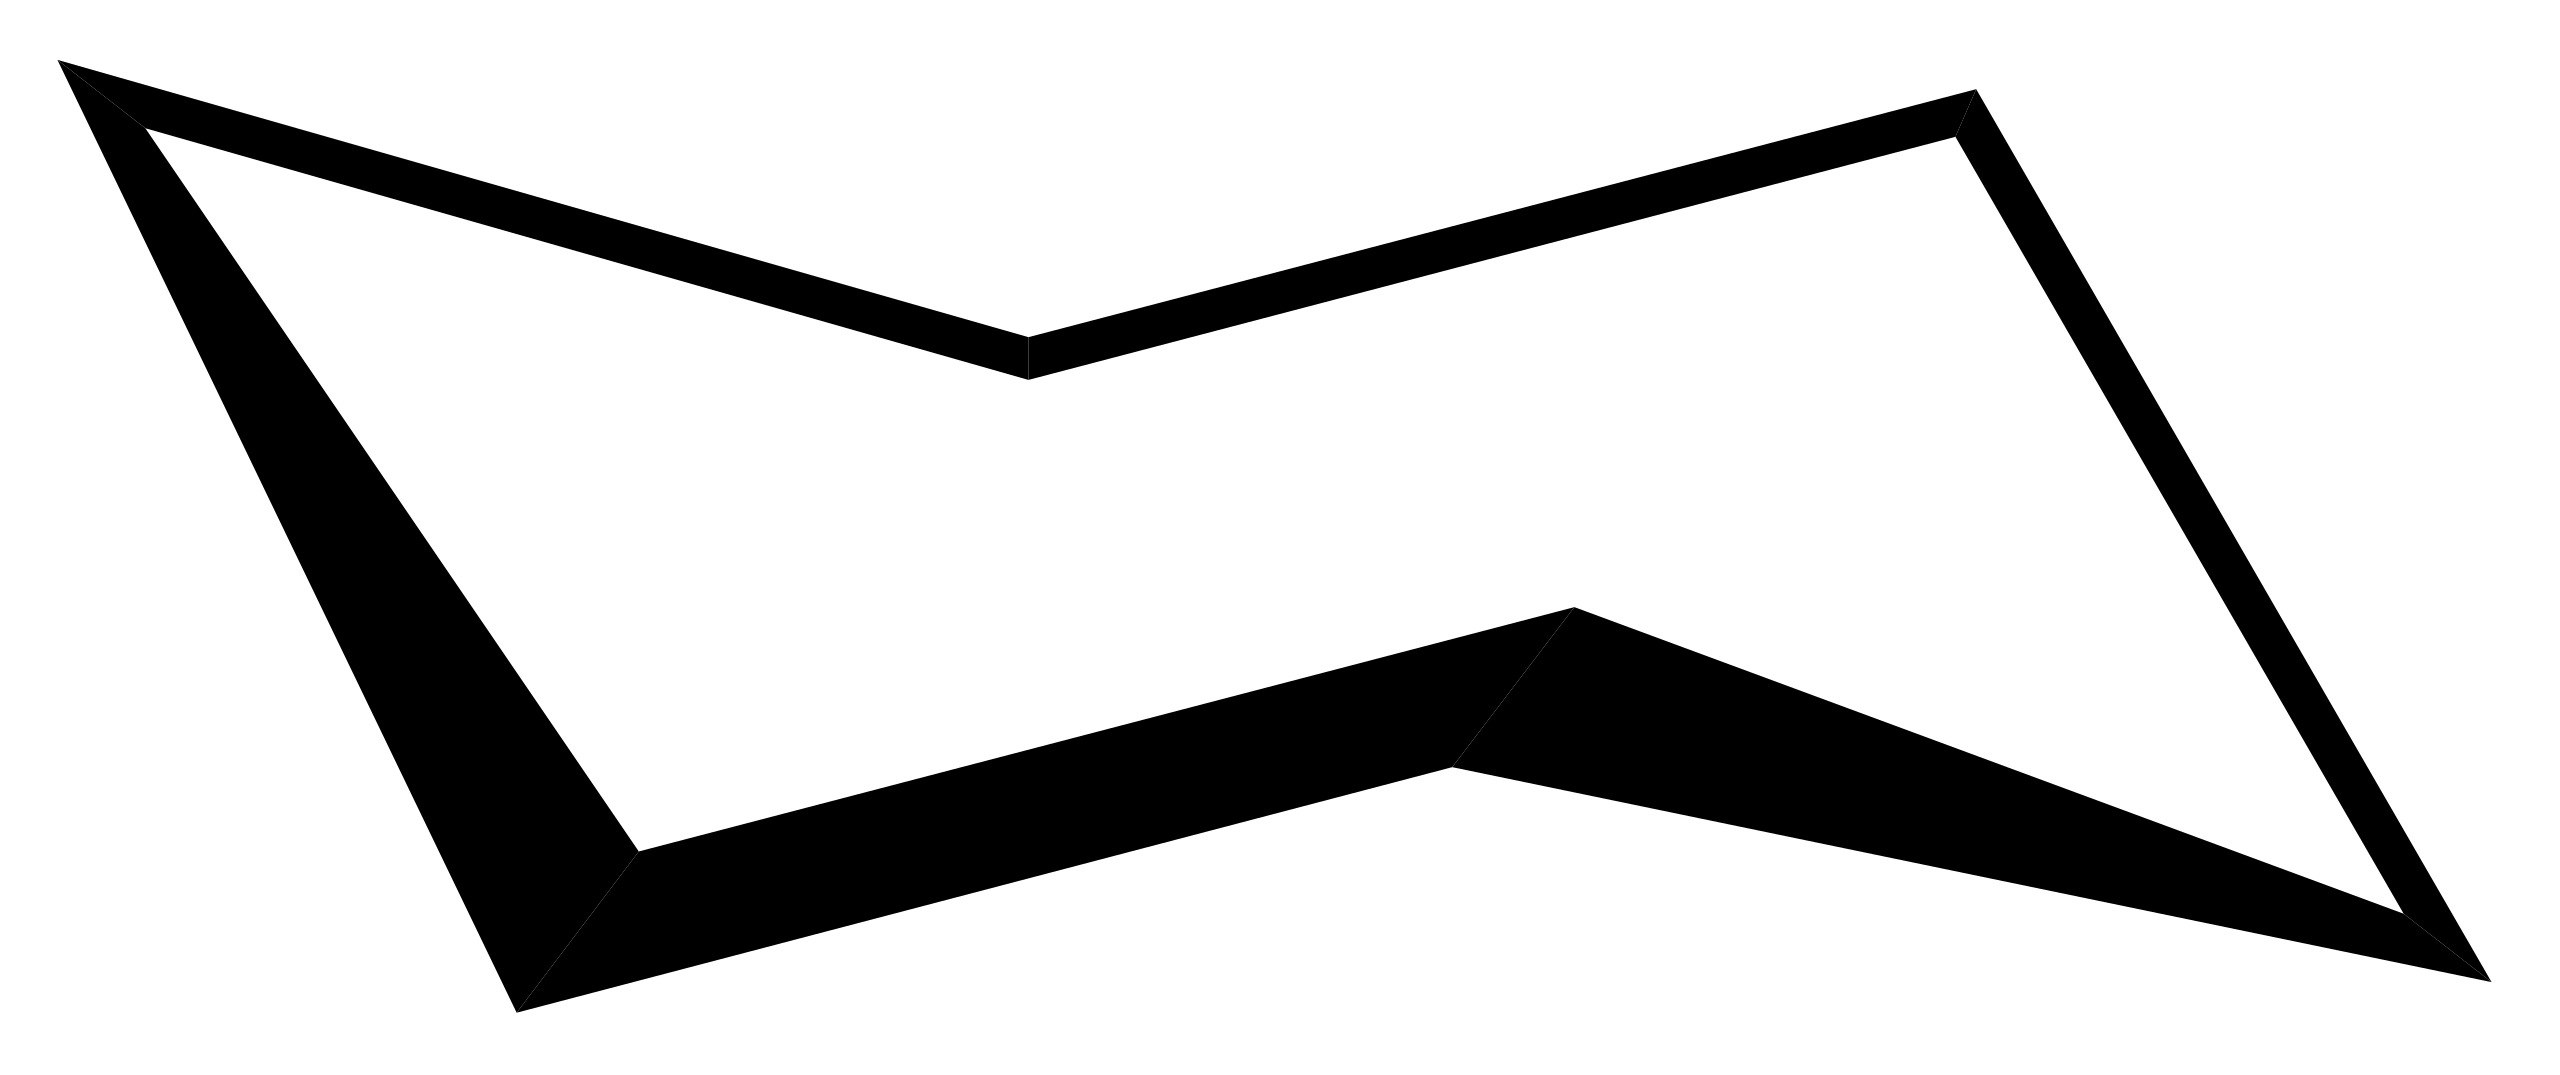
\includegraphics[scale=0.1]{imagens/2560px-Chair_conformation_of_cyclohexane.svg.png}
\label{fig:cicloexano}\vspace{0.5cm}\end{figure}

A figura \ref{fig:cicloexano} apresenta um dos mais belos e complexos temas da Química Orgânica: os fundamentos da análise conformacional. Analisar a forma tridimensional de uma molécula é fundamental para compreender sua interação com outras moléculas ou então com substratos biológicos. Em tal representação, as ligações Carbono-Hidrogênio são omitidas por clareza e as ligações Carbono-Carbono são representadas por um traço. Na figura vemos traços mais grossos que outro, usados aqui para fornecer uma ideia tridimensional em um veículo nitidamente bidimensional, este livro. Assuma quem, quando um traço estiver mais grosso, os átomos envolvidos estão espacialmente mais próximos do leitor do que os demais.

Além dessas categorias, a aromaticidade é uma propriedade especial observada em alguns hidrocarbonetos, como o benzeno. Moléculas consideradas aromáticas apresentam uma estabilidade excepcional devido ao fenômeno conhecido por ressonância eletrônica em seu sistema de anel, tornando-as distintas das categorias mencionadas anteriormente.

A classificação de hidrocarbonetos é essencial na química orgânica, pois ajuda os químicos a compreenderem a estrutura, as propriedades e o comportamento desses compostos. Além disso, a capacidade de categorizar os hidrocarbonetos facilita a previsão de suas reações químicas e aplicações em diversas áreas, como indústria, farmácia e pesquisa científica. 

\section{Estrutura}
A representação estrutural de um hidrocarboneto, assim como nos demais compostos orgânicos, pode ser feita de diferentes formas, dependendo da finalidade ou necessidade específica. Como exemplo, podemos nos deparar com uma publicação científica que exige a representação de uma molécula com uso de pouco espaço, onde o foco não deve ser apenas na estrutura, mas no contexto global, como pôsteres em congressos.

As mais comuns representações moleculares em Química Orgânica são as seguintes:
\begin{itemize}
\item Fórmula estrutural completa
\item Fórmula estrutural condensada
\item Fórmula estrutural em bastão
\item Fórmula estrutural com preenchimento espacial
\end{itemize}

\section{Propriedades físicas de hidrocarbonetos}
Hidrocarbonetos são substâncias formadas apenas por átomos e carbono e átomos de hidrogênio, constituindo a espinha dorsal que pode originar muitas moléculas encontradas na natureza. Podem ser classificados em várias categorias, e suas propriedades físicas são importantes para compreender suas reações em condições naturais e industriais.

\subsection{Pontos de Fusão e Ebulição}

Os pontos de fusão dos hidrocarbonetos são afetados preferencialmente pelo número de átomos de carbono em suas moléculas e pelo arranjo topológico e espacial entre esses átomos. Os hidrocarbonetos classificados como saturados, como os alcanos, tendem a apresentar pontos de ebulição mais baixos, enquanto alcenos e alcinos (insaturados com ligação dupla ou tripla, respectivamente) tendem a apresentar pontos de ebulição mais elevados. A razão do auimento nos valores de PF é simples: sendo apolares, as moléculas dos hidrocabonetos atraem-se por meio das chamadas Forças de London, tipicamente fracas, mas à medida em que o número de átomos de carbono aumenta, tal atração torna-se acumulativamente mais significante e, portanto, os valores de PF aumentam. Veja um exemplo na tabela \ref*{pf} a seguir.

\begin{table}[!h]
\begin{center}
\caption{\label{pf}Temperaturas de fusão e ebulição de alguns hidrocarbonetos saturados.}
\vspace{0.5cm}
\begin{tabular}{|c|c|c|c|c|}
\hline
Substância & Fórmula & Massa molar (g/mol) & TF ({$^o$}C) & TE ({$^o$}C)\\
\hline
Metano & \ce{CH4} & 16 & -182 & -161 \\
\hline
Etano & \ce{C2H6} & 30 & -183 & -87 \\
\hline
Propano & \ce{C3H8} & 44 & -188 & -42 \\
\hline
Butano & \ce{C4H10} & 58 & -138 & -0,5 \\
\hline
Pentano & \ce{C5H12} & 72 & -130 & -36 \\
\hline
\end{tabular}
\end{center}
\end{table}

Os pontos de ebuilição dos hidrocarbonetos estão intimamente relacionados com o tamanho e a forma das moléculas. Por tal razão, dois hidrocarbonetos isômeros de cadeia (moléculas com mesma fórmula molecular, mas com cadeias carbônicas distintas), pentano e 2,2-dimetil-propano possuem Ponto de Ebulição tão distintos. A cadeia carbônica do pentano é normal (sem ramificações), enquanto a cadeia carbônica do 2,2-dimetil-propano é ramificada, o a faz tender a um formato esférico, com menor área superficial que o pentano. Assim, as forças de atração no poentano se tornam maiores e os PF são tão distintos, conforme pode ser visto na figura \ref{fig:pentano} a seguir.

\begin{figure}[H]
	\centering
	\caption{Influência da forma da molécula nos valore de PE}
	\vspace{0.5cm}
	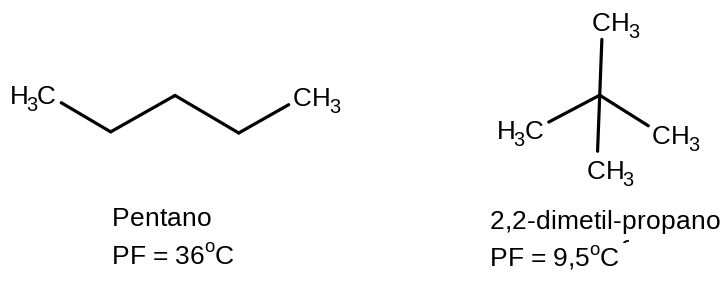
\includegraphics[width=1\linewidth]{imagens/pentano_22dimetil.png}
\label{fig:pentano}
\end{figure}


\subsection{Solubilidade}

A solubilidade dos hidrocarbonetos em água é geralmente muito baixa devido à natureza apolar de suas moléculas. No entanto, a solubilidade pode aumentar ligeiramente com o tamanho da cadeia crbônica, pois moléculas maiores possuem área superficial maior para interagir com as moléculas de água, mas isso só ocorre em poucas situações, como emulsões ou então quando óleo (mistura complexa de hidrocarbonetos) flutua na água.

A solubilidade é uma característica importante para a separação de hidrocarbonetos em processos de refino de petróleo e na indústria química. Sendo moléculas apolares, os hidrocarbonetos tendem a dissolver-se em moléculas igualmente apolares e, portanto, tendem a não interagir com água. Porém, dissolvem-se bem em solventes igualmente apolares, como benzeno (\ce{C6H6}).

De modo geral, hidrocarbonetos de cadeias curtas são mais solúveis em solventes apolares do que hidrocarbonetos de cadeia carbônica maior, pois moléculas menores podem dispersar-se melhor entre as moléculas do solvente. A ramificação das cadeias carbônicas dos hidrocarbonetos pode aumntar sua solubilidade em solventes apolares, uma vez que a área superficial é reduzida e uma molécula compacta dispersa-se melhor que uma molécula maior.

 

\subsection{Densidade}
A densidade de hidrocarbonetos varia com sua composiçao e estrutura molecular. Normalmente, os HC mais leves, como metano (\ce{C4}) ou etano (\ce{C2H6}) saõ menos densos que o ar, são inflamáveis e tendem a ascender, uma vez que todo gás menos denso que o ar sofre esse fenônemo. A densidade é uma característica  importante em processos de separação, como a destilação, através da qual os componentes são separados com base em suas diferenças de densidade. De modo geral, quanto maior a massa molar de um hidrocarboneto, maior será sua densidade, uma vez que uma molécula mais pesada apresenta maior massa por unidade de volume. Como exemplo, o propano (\ce{C3H8}) apresenta densidade com valor \textbf{0,498 g/mL} enquanto o decano (\ce{C10H22}) apresenta densidade com valor \textbf{0,730 g/mL} na mesma temperatura de 20{$^o$}C.

\subsection{Tensão Superficial}
Em uma amostra de água, existem dois tipos de moléculas. As que estão por fora de uma dada gota, exteriores, e as que estão por dentro da mesma gota, interiores. As moléculas interiores são atraídas por todas as moléculas ao seu redor, enquanto as moléculas exteriores são atraídas apenas pelas outras moléculas da superfície e por aquelas abaixo da superfície. Isto faz com que o estado energético das moléculas no interior seja muito inferior ao das moléculas no exterior. Por causa disso, as moléculas tentam manter uma área superficial mínima, permitindo assim que mais moléculas tenham um estado de energia mais baixo. Isto é o que cria o que se conhece como tensão superficial. 

Em hidrocarbonetos, temos o mesmo comportamento, mas considerando as diferenças estruturais entre água e hidrocarbonetos. De forma geral, a tensão superficial aumenta com o aumento da massa molar do hidrocarboneto. Como exemplo, a substância conhecida como hexano (\ce{C6H14}) apresenta tensão superficial com valor 0,018 N/m \footnote{N/m é a unidade de tensão superficial: Newton/metro}, enquanto a água apresenta tensão superficial com valor 0,0720 N/m, quatro vezes maior que o hexano. A figura \ref{fig:ts} ilustra como as moléculas normalmente se organizam em fase líquida e mostra de modo simplificado como as forças atrativas ajudam a criar a rede superficial de moléculas.

\begin{figure}[H]
	\centering
	\caption{Composição de forças para a criação da Tensão Superficial}
	%\vspace{0.25cm}
	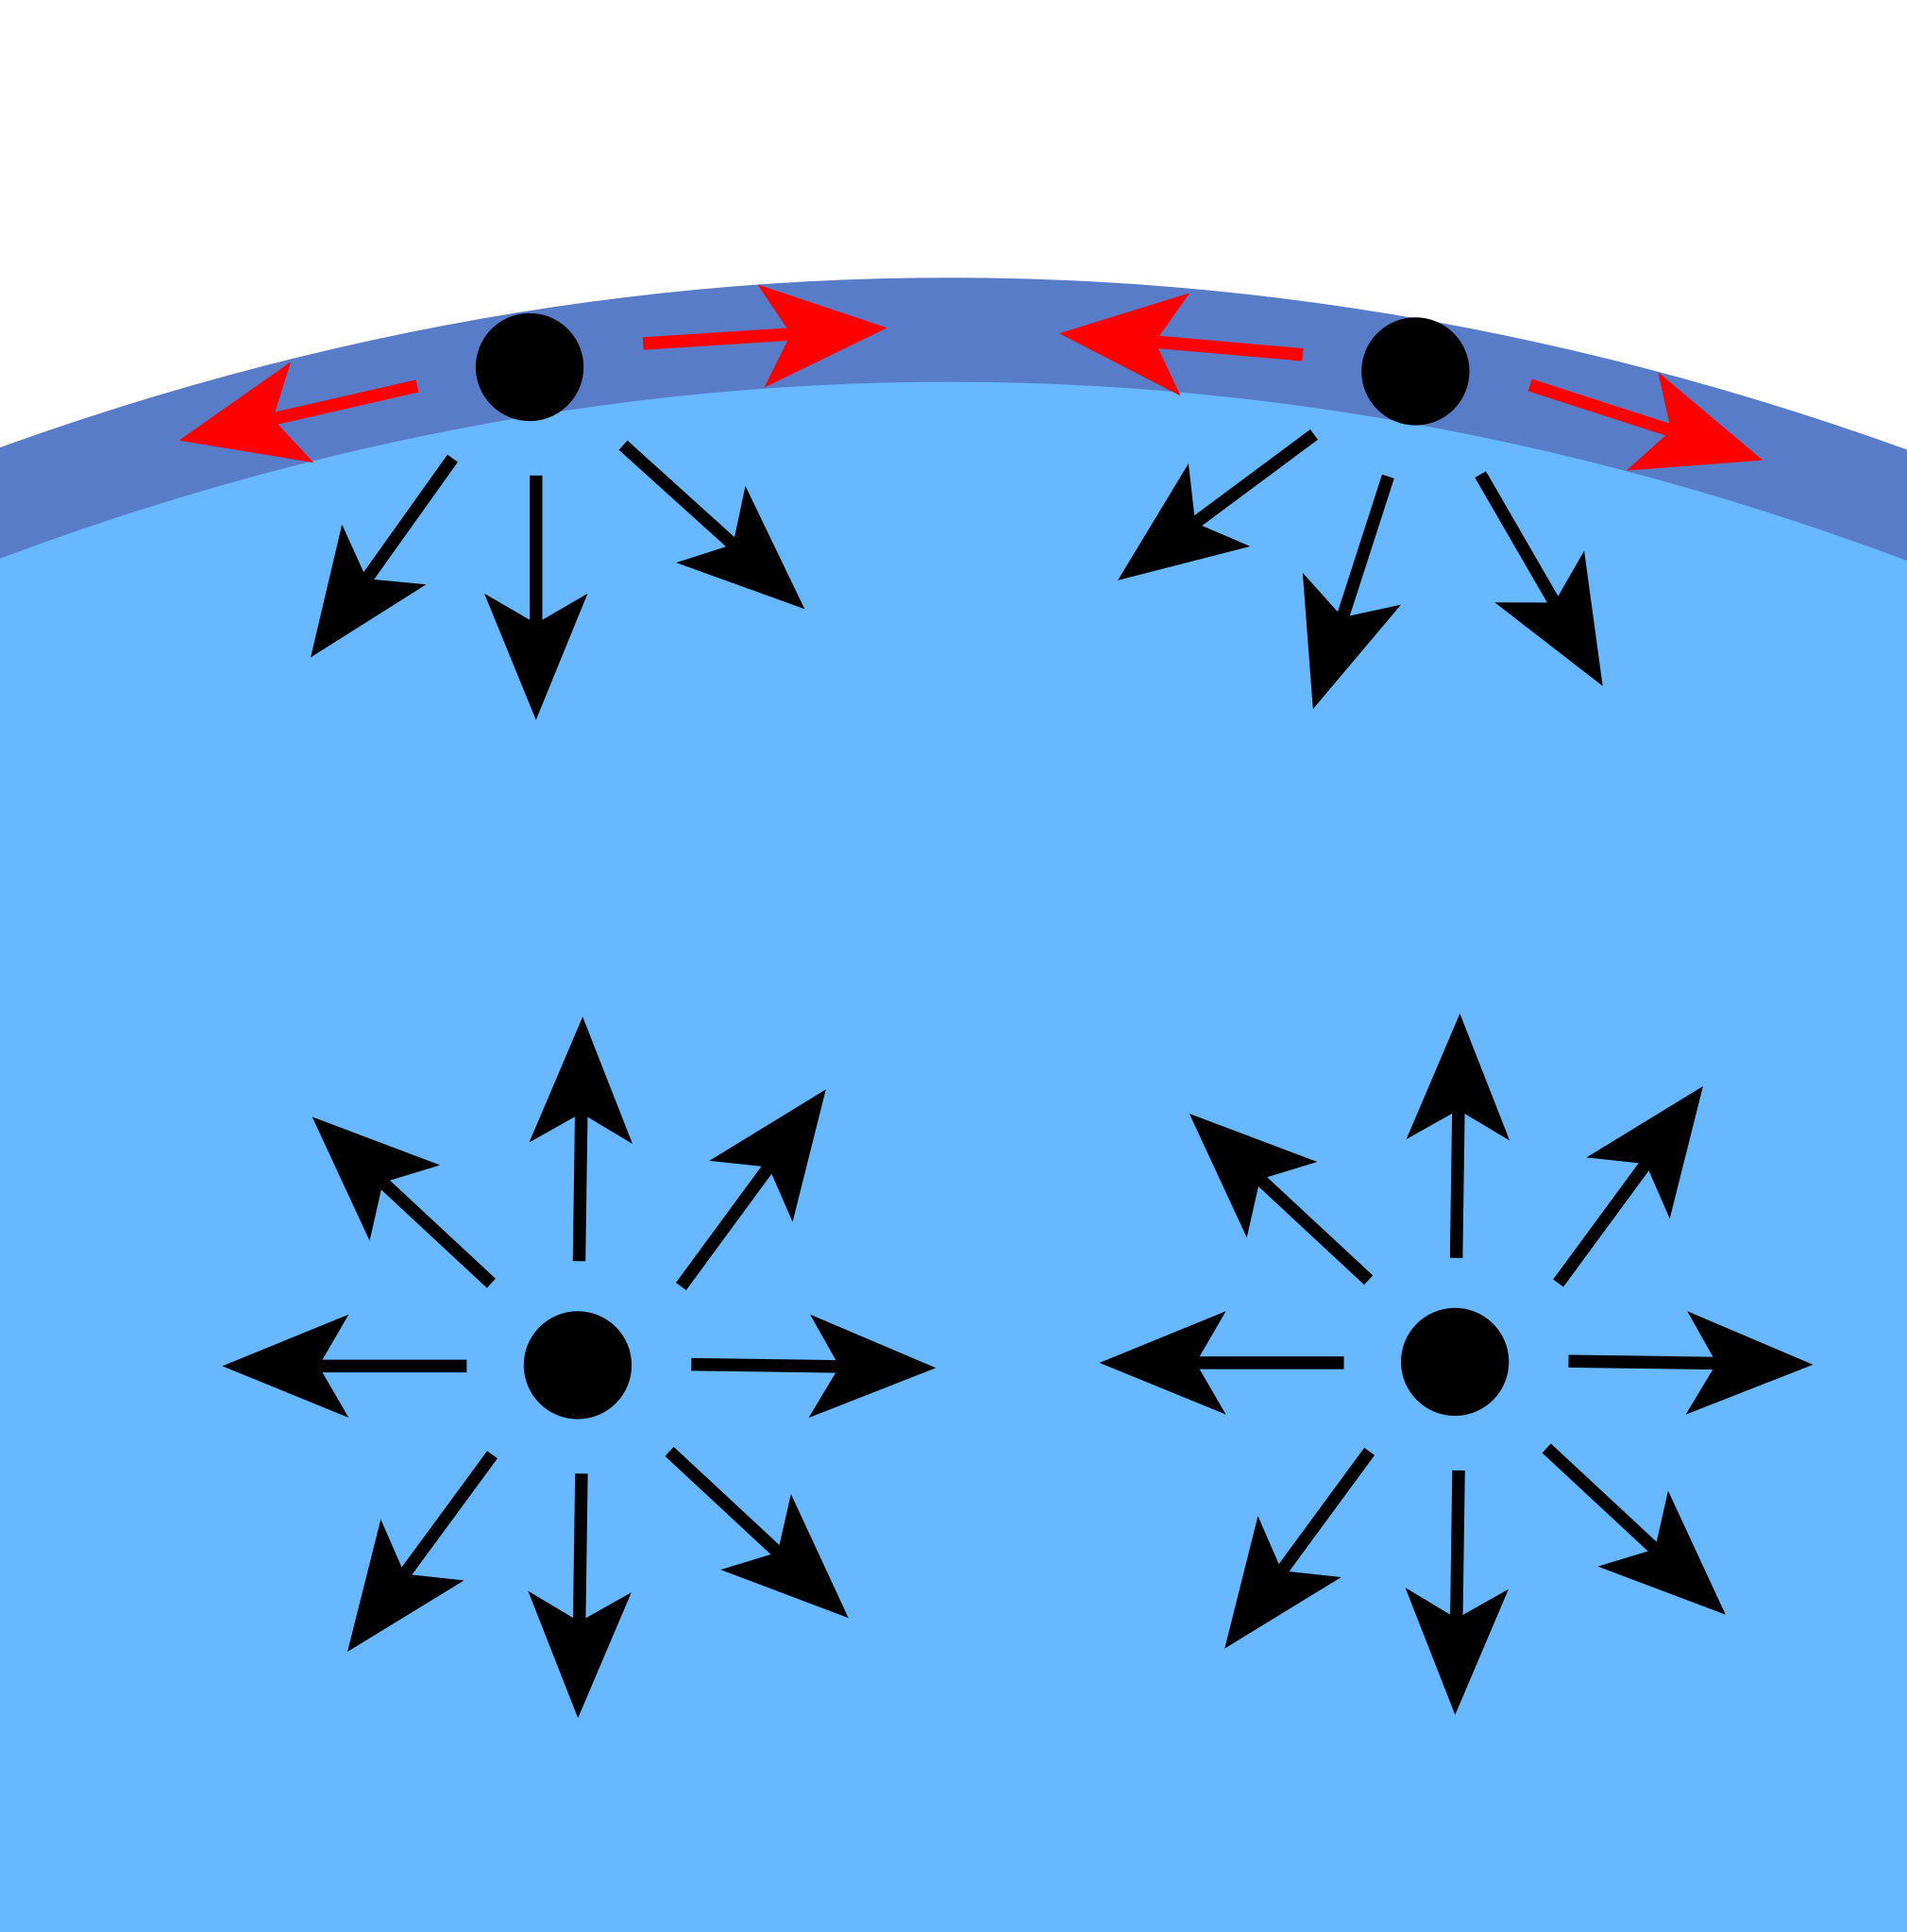
\includegraphics[width=0.35\linewidth]{imagens/ts.png}
	\caption*{Fonte: Wikipedia, disponível em https://shorturl.at/lrAGI}
\label{fig:ts}
\end{figure}

\section{Nomenclatura de hidrocarbonetos}
Assim como qualquer outra substância, todo hidrocarboneto precisa de ao menos dois conjuntos de informação: (a) uma fórmula que caracteriza suas propriedades e (b) um nome que define sua unicidade. Uma vez que são conhecidos centenas de milhares de hidrocarbonetos distintos, torna-se obrigatório o uso de alguma sistematização para criação de nomes únicos.

Esta imensa tarefa está centralizada na entidade conhecida como IUPAC (International Union for Pure and Applied Chemistry, ou União Internacional para Química Pura e Aplicada) e está registrada no chamado "BlueBook", documento específico para nomenclatura de substâncias orgânicas.

Devemos alertar o leitor que, uma vez que são conhecidas milhões de substâncias orgânicas, a quantidade de regras e orientações sugeridas pela IUPAC é relativamente grande e abordaremos neste documento, aos poucos, parte dessas regras, pois nossa obra tem escopo bem definido não necessita de todas as regras. Deixamos aqui a curiosidade do leitor na leitura das regras previstas na versão 3 do BlueBook.

\subsection{Nomenclatura substitutiva}
Este é o principal método utilizado para nomenclatura de substâncias orgânicas e, mais amplamente, para substâncias que possuam elementos dos grupos 13 a 17 da Classificação Periódica dos Elementos. De modo geral, uma substância orgânica tem seu nome construído a partir de regras sistemáticas para que cada nome seja inequívoco, utilizando ao menos dois elementos:

\begin{description}
	\item \textbf{Hidreto pai ou cadeia principal}: é uma substância formada apenas por uma dada cadeia carbônica, sem qualquer grupo funcional, seja com cadeia normal, ramificada, cíclica, aromática ou ainda heteregênea, conforme pode ser observado na figura \ref{fig:hp} a seguir.
	
	\begin{figure}[H]
		\centering
		\caption{Exemplos de hidretos pai}
		\vspace{0.5cm}
		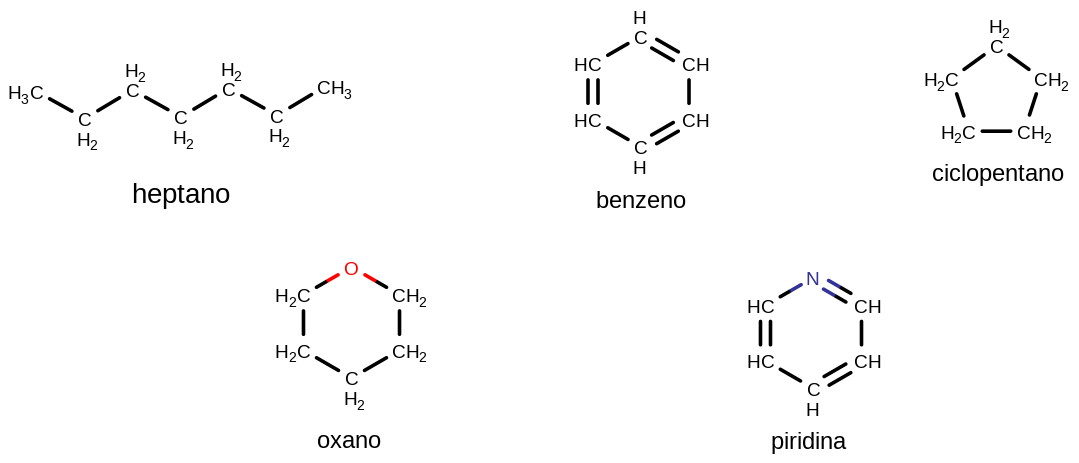
\includegraphics[width=1\linewidth]{imagens/hidretos_pai.png}
	\label{fig:hp}
	\end{figure}

	\item \textbf{Um grupo funcional principal}: caso a substância possua mais de um grupo funcional, um deles é o chamado \textbf{grupo funcional principal}, conforme pode ser visto na tabela \ref{senioridade} a seguir. As colunas "Prefixo" e "Sufixo" indicam, respectivamente, o nome de cada grupo funcional quando este não é a função principal (prefixo) e quando este é a função pricipal (sufixo).
\end{description}

Quando falamos da nomenclatura substitutiva, considere que um átomo de hidrogênio (por exemplo) tenha sido substituído por outro átom o ou grupo de átomos.

\begin{table}[!h]
	%\begin{tabular}
	\begin{center}
	\caption{\label{senioridade}Grupos funcionais em ordem decrescente de senioridade (prioridade)}
	\vspace{0.5cm}
	\begin{tabular}{l c c c}
	\hline
	Função orgânica& Fórmula & Prefixo & Sufixo\\
	\hline
	Carboxilatos & \ce{-COO$^-$} & carboxilato & alcoxicarbonil\\
	Ácido carboxílico & \ce{-COOH} & ácido carboxílico & carboxi\\
	Ésteres & \ce{-COOR} & R-oato & R-oxicarbonil\\
	Haletos de acila & \ce{-COOX} & oil haleto & halocarbonil\\
	Amidas & \ce{-COONH2} & amida & carbamoil\\
	Nitrilas & \ce{-CN} & nitrila & ciano\\
	Aldeídos & \ce{-COH} & al & oxo\\
	Cetonas & \ce{-CO-} & ona & oxo\\
	Álcoois & \ce{-OH} & ol & hidroxi\\
	Tióis & \ce{-SH} & tiol & sulfanil\\
	Aminas & \ce{-NH2} & amina & amino\\
	Iminas & \ce{=NH} & imina & imino\\
	\hline
	\end{tabular}
	\end{center}
\end{table}

\begin{tcolorbox}[colback=blue!5!white,colframe=gray!75!black,title=Atenção!]
	Embora esta seção {\thesection} trate da nomenclatura de hidrocarbonetos, ficam lançadas as bases para a nomenclatura de muitas outras funções orgânicas. Este livro não cobre todas as funções orgânicas conhecidas por tratar-se de de uma obra de caráter básico, e o trabalho de criação das regras de nomenclatura orgânica estende-se há anos a certamente perdurará por outros ainda.
  \end{tcolorbox}




Caso o hidreto pai possua algum grau de insaturação (ligações duplas ou triplas), o sufixo do hidreto se altaera para "eno" ou "ino", indicando as insaturações possível, com os localizadores adequados.

Naturalmente, a presença dos localizadores implica na necessidade da numeração da cadeia carbônica e, como consequência da presença de insaturação ou grupos funcionais, a numeração da cadeia igualmente segue regras bastante rígidas para manter a unicidade de cada nome.

A substância ilustrada abaixo, na figura \ref{fig:46} possui um nome construído pela nomenclatura substitutiva, onde átomos de hidrogênio foram substituídos de um dado hidreto pai.

\begin{figure}[H]
	\centering
	\caption{Exemplo de aplicação da nomenclatura substitutiva.}
	\vspace{0.5cm}
	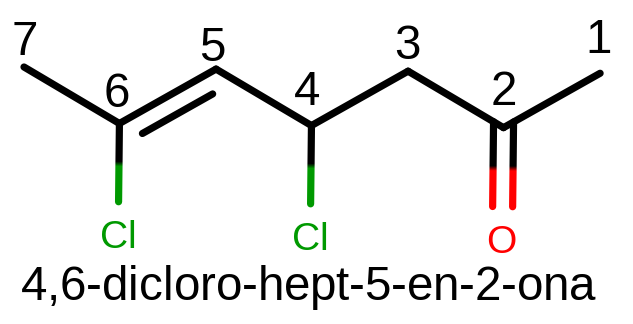
\includegraphics[width=0.6\linewidth]{imagens/46dicloro.png}
\label{fig:46}
\end{figure}

Podemos observar na figura que o hidreto pai consiste em uma cadeia carbônica com 7 átomos, com uma ligação dupla, o que por si só já exige a presença de localizadores, nos obrigando a numerar a cadeia carbônica, restando a dúvida de por onde a iniciar.

A numeração de um hideto pai (ou um copmposto pai, mais genericamente), deve ser efetuada por meio da aplicação dos seginte critérios:

\begin{enumerate}
	\item menor numeração possível para heteroátomos;
	\item menor numeração possível para hidrogênios indicados\footnote{Em determinadas circunstâncias é necessário indicar no nome de um anel, ou sistema de anéis, contendo o número máximo de ligações duplas não cumulativas, uma ou mais posições onde nenhuma ligação múltipla está anexada. Isso é feito especificando a presença de um átomo de hidrogênio 'extra' em tais posições pela citação do local numerado apropriado seguido por um H maiúsculo em itálico};
	\item menor posição possível para o grupo funcional principal;
	\item menor posição para insaturações;
	\item menor posição possível para substituintes indicados por prefixos;
	\item menor posição possível para substituintes em ordem de citação.
\end{enumerate}

Nossa próxima dúvida é a seguinte: por qual extremidade da cadeia com 7 átomos de carbono devemos iniciar a numeração? Consultando os dados presentes na tabela \ref{senioridade}, concluímos que o grupo funcional cetona possui maior senioridade (ou prioridade) na numeração, obedecendo o item 3 logo acima. Assim, a numeração do hidreto pai deve se iniciar na extremidade esquerda da cadeia, o que deixa, automaticamente, a ligação dupla na menor posição possível, restando apenas indicar a posição dos dois grupos funcionais (haleto) com menor prioridade, o que explica inequivocamente o nome da substância da figura \ref{fig:46}.

Analise o próximo exemplo, ilustrado na figura \ref{fig:octadieno} a seguir.

\begin{figure}[H]
	\centering
	\caption{Exemplo de aplicação da nomenclatura substitutiva.}
	\vspace{0.5cm}
	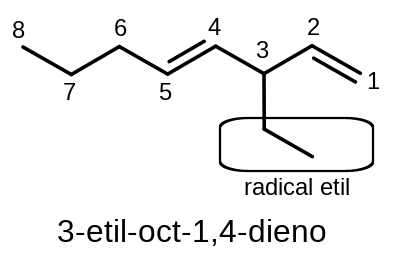
\includegraphics[width=0.6\linewidth]{imagens/octadieno.png}
\label{fig:octadieno}
\end{figure}

Como trata-se de um hidrocarboneto, não há grupos funcioniais na disputa por senioridade, deixando a discussão apenas para decisão entre os radicais substitutintes e as insaturações. Como estas últimas possuem maior senioridade que os radicais, a nmewração da cadeia deve iniciar-se em uma extremidade que deixa as insaturações nas memores posições possíveis da numeração. Finalmene, existe um radical \textbf{etil} conectado ao carbono 3 do hidreto pai. Assim, o nome da substância é \textbf{3-etil-oct-1,4-dieno}. 

Finalizando, convidamos o leitor a examinar a estrutura a seguir, na figura \ref{fig:etenil}, e identificar o número de átomos de carbono do hidreto pai.

\begin{figure}[H]
	\centering
	\caption{Exemplo de aplicação da nomenclatura substitutiva.}
	\vspace{0.5cm}
	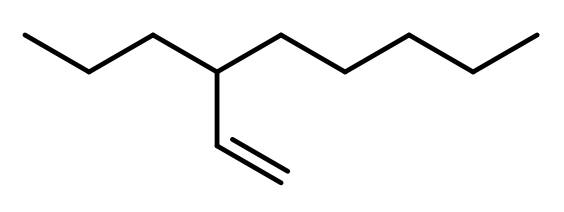
\includegraphics[width=0.6\linewidth]{imagens/etenil.png}
\label{fig:etenil}
\end{figure}

Recomendações da IUPAC anteriores a 2013 sugeriam que o hidreto pai deveria conter eventuais insaturações, mas a recomendação mais atual sugere que o hidreto pai seja aquele com maior número de átomos de carbono, contendo ou não a insaturação. Portanto, o nome da substância da figura \ref{fig:etenil} é mostrado a seguir.

\begin{figure}[H]
	\centering
	\caption{Exemplo de aplicação da nomenclatura substitutiva.}
	\vspace{0.5cm}
	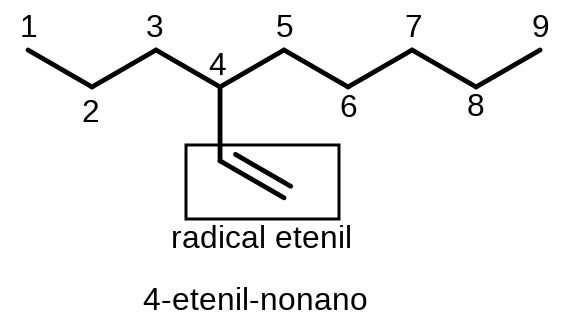
\includegraphics[width=0.6\linewidth]{imagens/nomeetenil.png}
\label{fig:nomeetenil}
\end{figure}

\chapter{Álcoois e fenóis}
\begin{mdframed}[backgroundcolor=orange!20,linewidth=0pt,roundcorner=10pt]
	\minitoc
\end{mdframed}
Após analisar funções orgânicas contendo apenas Carbono e Hidrogênio em suas moléculas, focamos nossa atenção em funções contendo o grupo \textbf{hidroxil} (OH) ligado a dois tipos de átomos de Carbono, o que origina duas funções distintas: \textbf{álcoois} (grupo hidroxil ligado a carbono saturado) e \textbf{fenóis} (grupo hidroxil ligado a carbono aromático), conforme pode ser visto na figura \ref{fig:af}

\begin{figure}[H]
	\centering
	\caption{Exemplo de substância da função álcool (glicerol) e de substância da função fenol (hidroquinona). Os nomes citados são \textbf{usuais}.}
	\vspace{0.5cm}
	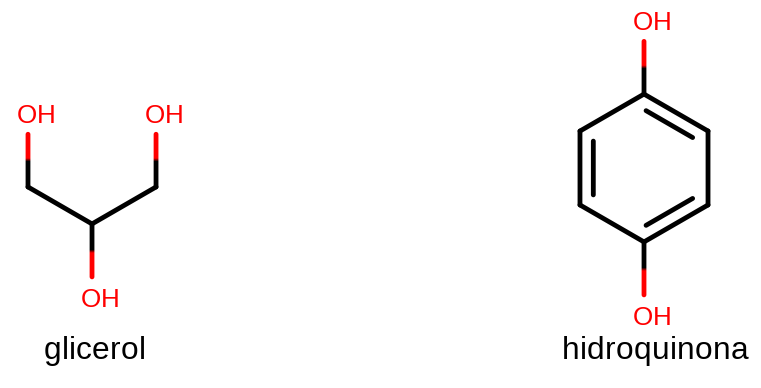
\includegraphics[width=0.7\linewidth]{imagens/af.png}
	\label{fig:af}
\end{figure}


Estas funções são bastante versáteis quando de trata de síntese orgânica, ou seja, reações orgânicas que permitem a obtenção de medicamentos, corantes, plásticos, entre muitas outras classes de substâncias orgânicas, o que lhes confere importância econômica quando pensamos em atividades industriais.

\section{Aspectos estruturais}
Podemos representar, de modo genérico, um álcool pela fórmula geral R-OH, onde R é um radical alquil (metil, etil, isopropil, entre outros) enquanto um fenol é representado pela fórmula geral ArOH, onde Ar é um radical aril (aromático), como fenil, naftil, entre outros.

Em termos estruturais, álcoois e fenóis são, simultaneamente, semelhantes e distintos, pois a presença do grupo OH ligado diretamente a um carbono saturado (álcoois) ou diretamente a um carbono aromático (fenóis) confere propriedades e reatividades distintas às duas funções.

Álcoois apresentam uma característica estrutural muito importante e que ajuda a explicar boa parte de suas propriedades: a possibilidade de formaçào de ligações de hidrogênio com água. A figura \ref{fig:ligacaoh}  ilustra a formação dessa ligação entre etanol (esquerda) e água (direita), \textbf{indicada pelo tracejado entre as duas moléculas}. Nesta representação, o átomo de carbono é a bola de cor cinza (maior), o hidrogênio é a bola branca (menor) e o átomo de oxigênio é a bola vermelha (tamanho intermediário).

 \begin{figure}[h]
	\centering
	\caption{Ligação de hidrogênio entre etanol e água, desenhada usando o software Avogadro \cite{avogadro}}
	\vspace{0.5cm}
	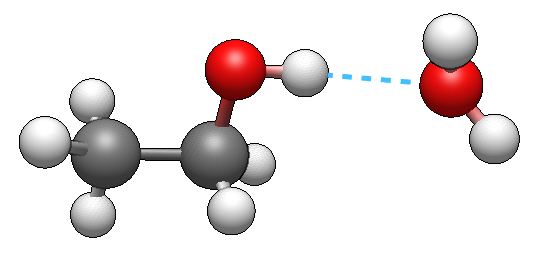
\includegraphics[width=0.65\linewidth]{imagens/ligacaoh.png}
	\label{fig:ligacaoh}
\end{figure}

\subsection{Caráter ácido/base}

Isoladamente, as moléculas de propanol e de fenol, usadas adiante como exemplo, são analisadas sem a presença de água ou qualquer outro solvente, apenas para ilustrar os efeitos decorrentes da presença do grupo OH nas duas funções. Por uma questão de simplicidade, usaremos apenas a propriedade periódica conhecida como \textbf{eletronegatividade}, juntamente com a \textbf{ressonância}, discutida anteriormente, para explicar as diferenças no caráter ácido/base do etanol e do fenol.

Parte da análise feita nesta seção utiliza o conceito de \textbf{pKa}, uma medida da ionização de uma substância quando encontra-se em solução aquosa.

A definição conceitual de pKa é a constante de equilíbrio de ionização de um ácido fraco, é uma medida da força de um ácido fraco. Quanto menor o pKa, mais forte é o ácido. Em termos mais simples, o pKa é o pH em que a concentração de ácido não ionizado é igual à concentração de ácido ionizado.

Por exemplo, o ácido acético, exibido na figura \ref{fig:ionizacao}, presenta valor de pKa igual a 4,76. Isso significa que, em uma solução aquosa com pH de 4,76, a concentração de ácido acético não ionizado é igual à concentração de ácido acético ionizado. Em pHs mais baixos, o ácido acético está mais protonado, ou seja, na forma de ácido. Em pHs mais altos, o ácido acético está mais desprotonado, ou seja, na forma de base.

\begin{figure}[h]
\centering
\caption{Exemplo da ionização de um ácido fraco}
\vspace{0.25cm}
\label{fig:ionizacao}
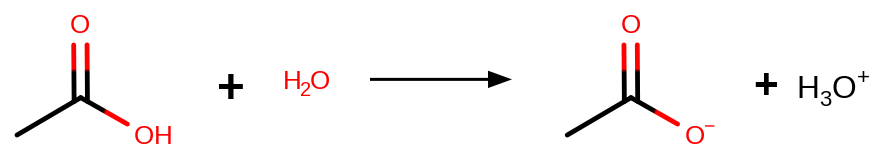
\includegraphics[width=0.9\linewidth]{imagens/ionizacao.png}
\caption*{Fonte: Autores}
\end{figure}

Matematicamente, temos:
\begin{equation}
	pK_ a = -log(K_ a)
\end{equation}

onde Ka é o valor da constante de equilíbrio de ionização do ácido acético:
\begin{equation}
	K_a = \frac{{\left[ {H_3O^ + } \right]\left[ {Ac^ - } \right]}}{{\left[ {HAc} \right]}}
	\label{eq:ionizacao}
\end{equation}

É importante notar, observando a equação \ref{eq:ionizacao}, que a quantidade em mol de água é muitísimo maior que todos os demais componentes do equilíbrio químico e está associada com K$_a$.

O átomo de oxigênio do grupo OH, nas duas funções aqui analisadas, encontra-se inicialmente com hibridização sp{$^3$} e apresenta uma relativamente elevada densidade eletrônica na região do grupo OH, conforme por ser observado nas figuras \ref{fig:subfenol} e \ref{fig:subpropanol} a seguir, que ilustram os mapas de potencial eletrostáticos para o fenol e o propanol.

Um mapa de potencial eletrostático é uma ferramenta de muito valiosa para visualizar a distribuição de cargas elétricas em uma molécula, bem como eventuais propriedades decorrentes desta disribuição de cargas.

A criação de um mapa de potencial eletrostático é normalmente feita com ajuda de um programa de computador por causa da enorme quantidade de operações matemáticas que devem ser feitas para calcular a energia potencia eletrostática nos diversos pontos da molécula, usando métodos derivados da Equação de Schrödinger \cite{Schrodinger}.

A visualização do mapa de potencial eletrostático é feita usando, por exemplo, uma paleta ou espectro de cores, normalmente usando a cor vermelha para menor potencial eletrostático e azul para maior potencial eletrostático.

Analisando a figura  com mais detalhes, podemos perceber uma região de cor vermelha próxima ao átomo de Oxigênio da função fenol, o que indica densidade eletrônica mais alta naquela região, compatível com a espécie \textbf{fenolato} que se forma na ionização do fenol em água.

\begin{figure}[H]
	\caption{Mapas de potencial eletrostático para fenol (a) e propanol (b)}
	\subfigure[Fenol]{\label{fig:subfenol}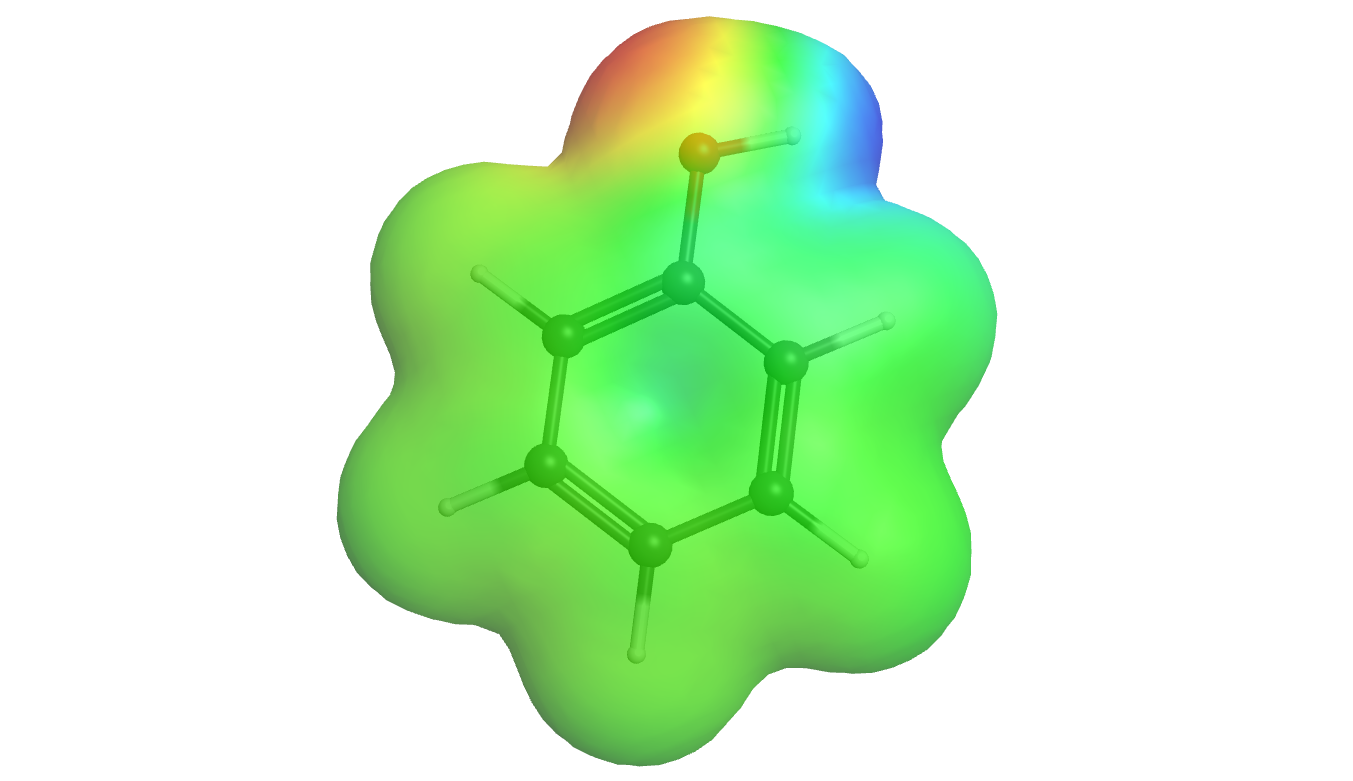
\includegraphics[width=90mm]{imagens/fenol.png}}
\hfill
	\subfigure[Propanol]{\label{fig:subpropanol}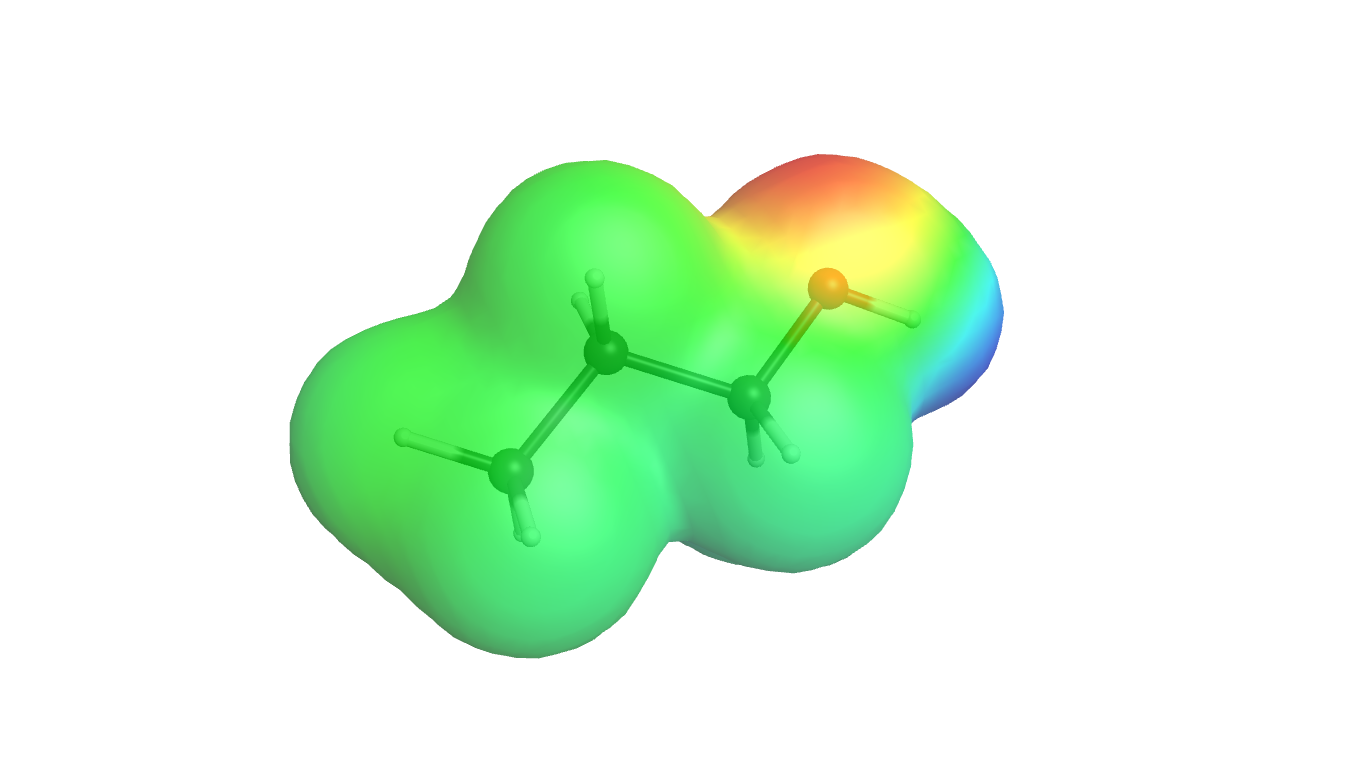
\includegraphics[width=90mm]{imagens/propanol.png}}
	\label{fig:subgraficos}
\end{figure}

A formação do íon fenolato em água ocorre através de um processo conhecido por ionização, ilustrado na figura \ref{fig:ionizacao}. Uma vez que a ligação H-O no fenol é bastante polarizada, conforme pode ser evidenciado no mapa de potencial eletrostático mostrado figura \ref{fig:subgraficos}, a quebra heterolítica da ligação H-O, provocada por ação da água, é facilitada.

O conceito de \textbf{ressonância} ajuda muito na compreensão do caráter ácido do fenol por causa da deslocalização da carga negativa do íon fenolato por meio do sistema aromático, conforme pode ser visto na figura \ref{fig:fenolfenolato}.

\begin{figure}[h]
\centering
\caption{Ionização do fenol, com estruturas de ressonância}
\vspace{0.5cm}
\label{fig:fenolfenolato}
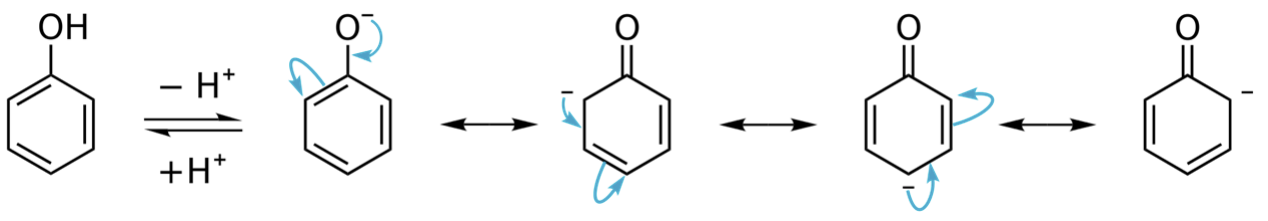
\includegraphics[width=1\linewidth]{imagens/fenolato.png}
\caption*{Fonte: Universidade de São Paulo, disponível em https://shorturl.at/fjrX8}
\end{figure}

A figura \ref{fig:fenolfenolato} esclarece as razões pelas quais o íon fenolato é estável e, portanto, o fenol apresenta caráter ácido. Da esquerda para a direita, temos o fenol perdendo um cátion H$^+$ por ionização em água e convertendo-se no íon fenolato, caracterizado por uma carga elétrica negativa no átomo de oxigênio. As setas indicam a movimentação dos elétrons no sistema conjugado do anel aromático, conforma descrito em -inserir refrência sobre ressonância-.
Repare que as ligações covalentes duplas tem suas posições alteradas por duas características peculiares do sistema aromático: \textbf{(a)} planaridade dos átomos do anel aromático e \textbf{(b)} presença de orbitais p puros, possibilitando a ressonância e a consequente deslocalização da carga negativa ao longo do ciclo aromático.

Comparado com o fenol (pK$_a$ = 10), etanol ou propanol (ambos com pK$_a$ = 16) \textbf{não possuem quaisquer resquisitos estruturais para estabilização da carga negativa} no átomo de Oxigênio e, portanto, não apresentam caráter ácido.

\subsection{Propriedades físicas}
Álcoois como metanol, etanol e propanol são totalmente solúveis em água por razões tratadas anteriormente, mas à medida em que aumenta o número de átomos de Carbono da cadeia, a solubilidade em água diminui em função do aumento da contribuição da cadeia carbônica, essencialmente apolar, minimizando a ação das ligações de hidrogênio possíveis entre o grupo hidroxil e água. Assim o butanol é menos solúvel em agua em relação aos álcoois de menor cadeia carbônica. Analisando a tabela \ref{solubilidade}, percebemos a influência da cadeia carbônica na solubilidade de alguns álcoois em dois solventes muito comuns: água (para substâncias polares) e hexano (para substâncias apolares). Cadeias carbônicas maiores fazem com que o álcool tenha solubilidade muito reduzida e comporte-se quase como um hidrocarboneto. Para que ocorra a dissolução do álcool, é necessário que as ligações de hidrogênio entre o álcool/água rompam as ligações de hidrogênio água/água, o que não ocorre em álcoois de cadeia carbôncia maior.

\begin{table}[!h]
	\begin{center}
	\caption{\label{solubilidade}Solubilidade de alguns álcoois em água e hexano (g/100g de solvente)\cite{solubilidade}}
	\vspace{0.5cm}
	\begin{tabular}{l c c}
	\hline
	Nome & Solubilidade em água & Solubilidade em hexano\\
	\hline
	Metanol & $\infty$ & 3,8\\
    %\hline
	Etanol & $\infty$ & $\infty$\\
	%\hline
    Propanol & $\infty$ & $\infty$\\
	Butanol & 7,9 & $\infty$\\
	Heptanol & 0,2 & $\infty$\\
    \hline
	\end{tabular}
	\end{center}
	\caption*{Fonte: referência \cite{solubilidade}}
\end{table}

Por outro lado, fenóis apresentam cadeia carbônica superior a vários álcoois e, portanto, possuem solubilidade menor, mas preciusamos considerar o efeito da ionizaçãod e fenóis em água, discutido anteriormente, e que ajuda a explicar a maior solubilidadede do, por exemplo, fenol comparado com um álcool de massa molar próxima, conforme pode ser visto na tabela \ref{comparada}.

\begin{table}[!h]
	\begin{center}
	\caption{\label{comparada}Solubilidade comparada do fenol e do pentanol}
	\vspace{0.5cm}
	\begin{tabular}{l c c c}
	\hline
	Nome & Massa molar (g/mol) &Solubilidade em água & Solubilidade em hexano\\
	\hline
	Fenol & 94 & 8,0 & 3,8\\
    %\hline
	Pentanol & 88 & 2,3 & $\infty$\\
	Hexanol & 102 & 0,6 & $\infty$\\
    \hline
	\end{tabular}
	\end{center}
	\caption*{Fonte: Autores}
\end{table}

O ponto de ebulição de álcoois varia de acordo com o tamanho da cadeia carbônica, como pode ser observado na figura \ref{fig:ebulicao}, e o ponto de ebulição de fenóis varia aproximadamente da mesma forma \cite{fisicas}.

\begin{figure}[h]
	\caption{Ponto de ebulição de alguns álcoois em função cadeia carbônica (\textcelsius)}
	\label{fig:ebulicao}
	
	\vspace{0.5cm}
	\centering
\begin{tikzpicture}
	\begin{axis}[
		title={},
		xlabel={Tamanho cadeia carbônica / átomos},
		ylabel={Temperatura de ebulição / \textcelsius},
		xmin=0, xmax=11,
		ymin=40, ymax=240,
		xtick={1,2,3,4,5,6,7,8,9,10},
		ytick={65,78,97,118,138,157,178,195,214,229},
		legend pos=north west,
		ymajorgrids=true,
		grid style=dashed,
	]
	\addplot[
		color=blue,
		mark=square,]
		coordinates {(1,65)(2,78)(3,97)(4,118)(5,138)(6,157)(7,178)(8,195)(9,214)(10,229)};
		\legend{}
	\end{axis}
\end{tikzpicture}
	\caption*{Fonte: Autores}
\end{figure}

%\section{Obtenção e usos}
\section{Ocorrência e aplicações}
Conforme já mencionado no início deste capítulo, álcoois e fenóis são compostos versáteis e muito úteis em diversos setores econômicos e industriais, e considerando o etanol como um dos protagonistas, por suas aplicações variando de componente de bebidas até combustíveis automotivos, passando por produtos de limpeza, tanto domésticos quanto hospitalares.

\subsection{Álcoois}
Muitos exemplos de substâncias pertencentes à função álcool possuem usos biológicos e/ou aplicações industriais e podemos fixar nossa análise em compostos monofuncionais, ou seja, possuem apenas a função álcool.

\subsubsection{Metanol}
Assim, o mais simples dos álcoois, o composto de fórmula \ce{CH3OH} recebe o nome de metanol, pois possui apenas um carbono e o hidreto pai é o metano. Pela nomenclatura substitutiva, um átomo de Hidrogênio foi substituído pelo grupo OH e álcoois possuem o sufixo ol. Justificado o nome \textbf{metanol}, certo?

\begin{figure}[h]
    \centering
    \caption{Fórmula estrutural para o metanol}
    \vspace{0.5cm}
    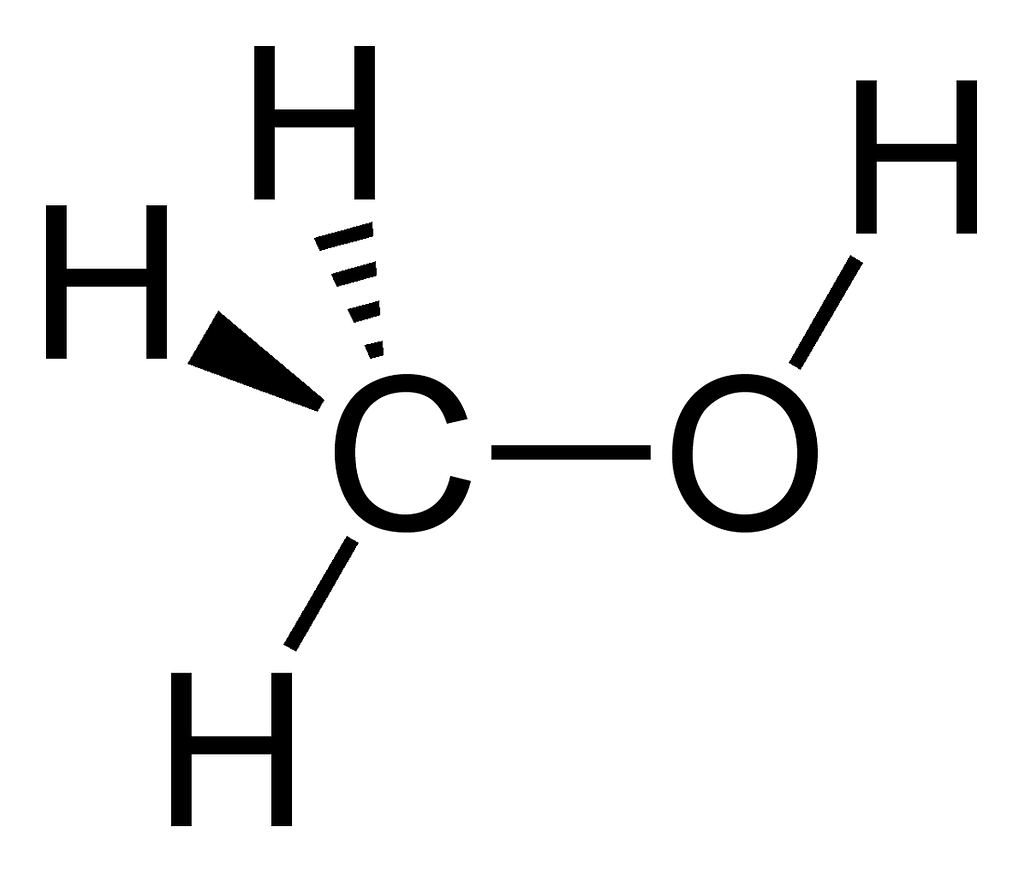
\includegraphics[width=0.2\linewidth]{imagens/methanol-2d-0349e4-1024.png}
\label{fig:mpemetanol}
\end{figure}

A figura \ref{fig:mpemetanol} a seguir ilustra o mapa de potencial eletrostático para o metanol e tal mapa indica a distribuição de cargas elétricas na substância, utilizando uma paleta de cores que vai do azul ao vermelho, onde este último indica maior quantidade de carga em uma dada região, comparada com a cor azul de outra região.

\begin{figure}[h]
    \centering
    \caption{Mapa de potencial eletrostático para o metanol}
    \vspace{0.5cm}
    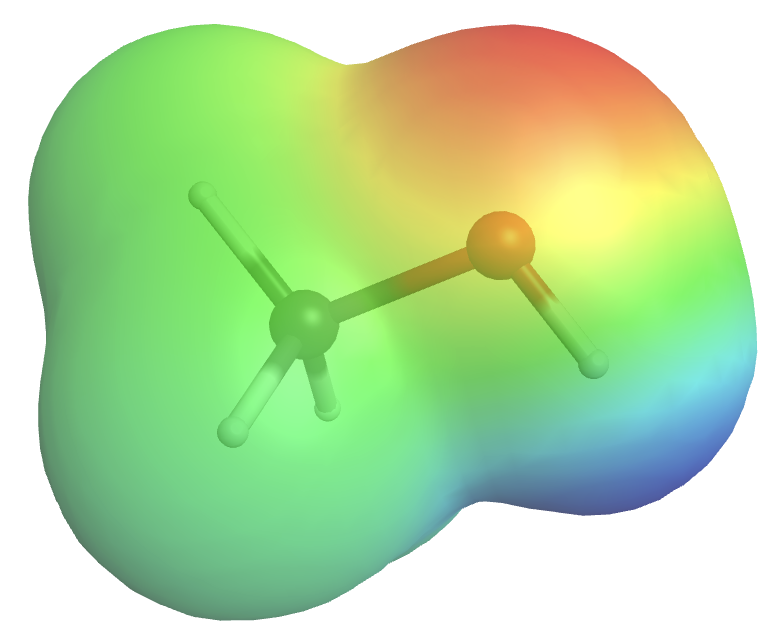
\includegraphics[width=0.45\linewidth]{imagens/mpemetanol.png}
\label{fig:mpemetanol}
\end{figure}

Um estudo recente realizado no Brasil \cite{D2CC01757A} mostra a foto-oxidação de metano para produzir metanol em condições ambientes, catalisada por metais de transição. Comparado com métodos clássicos, as condições reacionais e a possibilidade de uso de luz solar no processo tornam esse estudo muito promissor na produção em escala industrial de metanol.

A toxicidade do metanol, indicada pelo Diagrama de Hommel, indicado na figura \ref{fig:hommel} a seguir, pode ser analisada considerando as quatro partes da imagem contendo números inteiros em uma escala entre 0 e 4, onde 0 indica ausência de problemas e 4 indica perigo crítico.

A figura geométrica do losango é usada pela NFPA (National Fire Protection Association) \footnote{Veja mais em https://www.nfpa.org/codes-and-standards/7/0/4/704}, nos Estados Unidos da América, para indicar riscos associados a cada substância cadastrada na instituição.

A parte em cor vermelha (porção superior do losango) indica a \textbf{inflamabilidade} da substância, ou seja, sua capacidade de entrar em combustão. Portanto, o metanol é bastante inflamável e com um seríssimo agravante: sua combustão gera chamas de cor azul muito claras e visíveis apenas à noite, exigindo mais cuidados em sua manipulação. Diversos acidentes envolvendo metanol já foram citados e aqueles envolvendo automóveis de corrida da chamada Fórmula Indy, categoria automobilística muito famosa nos Estados Unidos da América, são chocantes \footnote{Veja mais em https://www.essentiallysports.com/nascar-news-invisible-fire-at-the-nineteen-eighty-one-indy-five-hundred-sets-the-nascar-community-ablaze-after-fans-make-talladega-superspeedway-nights-connection/}.

A parte em cor azul (porção central e esquerda do losango) indica o \textbf{risco à saúde} e, portanto, o contato ou ingestão deve ser evitado. Para referência, a dose letal por via oral em ratos é de pouco mais de 5,6 g/kg de peso corporal.

A parte em cor amarela (porção central direita do losango) indica \textbf{instabilidade ou reatividade} e mostra a estabilidade do metanol.

A parte em cor branca (porção inferior do losango) indica \textbf{risco específico} (oxidante forte ou radioativo, por exemplo) e não há registros de tal categoria para o metanol.


\begin{figure}[h]
    \centering
    \caption{Diagrama de Hommel para o metanol}
    \vspace{0.5cm}
    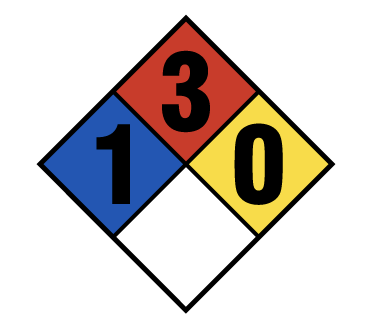
\includegraphics[width=0.25\linewidth]{imagens/hommel.png}
\label{fig:hommel}
\end{figure}

\subsubsection{Etanol}
Este álcool possui tamanha importância no Brasil, seja como combustível, como componente de produtos de limpeza ou em bebidas alcoólicas, que seu nome se confunde com a função orgânica à qual pertence \cite{raizen}. Por muito tempo os brasileiros compravam "álcool" em postos de combustíveis e apenas recentemente a substância passa a ser comercializada com seu nome oficial.

Trata-se de um líquido transparente, incolor, com densidade em torno de 0,8 g/cm$^3$ e miscível com água em qualquer proporção, explicado por meio da formação de ligações de hidrogênio entre água e etanol de modo tão intenso, que a mistura líquida é classificada como azeótropo, ou seja, os componentes da mistura entram em ebulição juntos, o que inviabiliza a destilação comum como meio de separação dos componentes desta mistura. Porém, é possível separar os componentes da mistura por outros métodos \cite{trica}.

\begin{figure}[h]
	\centering
	\caption{Diferentes representações para o etanol}
	\vspace{0.5cm}
	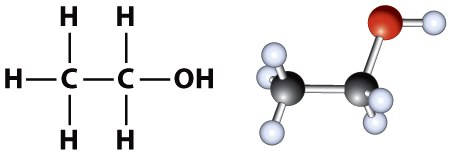
\includegraphics[width=0.75\linewidth]{imagens/etanol2.jpeg}
	\label{fig:etanol2}
\end{figure}

A figura \ref{fig:etanol2} ilustra ao menos duas representações distintas para o etanol: a fórmula estrutural completa (esquerda) e a representação do tipo "ball \& stick" (tubo e bola) (direita), onde as bolinhas de cores e/ou tamanhos diferentes representam os átomos e os tubinhos representam as ligações químicas entre eles. Existem diferentes representações para moléculas orgânicas em função do contexto de uso, onde uma dada representação pode ser mais esclarecedora que outra.

No Brasil, o etanol é produzido, essencialmente, por fermentação de sacarose por meio de leveduras, em inúmeras usinas de produção espalhadas pelo país, fato que movimenta um enorme número de trabalhadores nos diversos segmentos de produção e distribuição, alimentando uma cadeia produtiva bastante ampla.

Como é produzido a partir da sacarose obtida pela cana-de-açúcar, parte do dióxido de carbono, CO$_2$, produzido pela queima do etanol em motores a combustão, podemos dizer que o etanol é um combustível de ciclo neutro, conforme pode ser visto na figura \ref{fig:neutro} a seguir. Por "combustível de ciclo neutro", entenda, no caso do etanol, que sua principal fonte de obtenção é a cana-de-açúcar, vegetal com folhas verdes e capaz de realizar fotossíntese. Assim, a planta que origina o etanol captura parte das moléculas de CO$_2$ da atmosfera (algumas destas provenientes do etanol) e diminui os efeitos ambientais causados pela combustão do etanol como biocombustível.

\begin{tcolorbox}[colback=white!5!white,colframe=orange!90!black,title=\textbf{Equações de combustão do etanol (linha 1) e gasolina (linha 2)}]
	\ce{C2H6O + 3 O2 -> 2 CO2 + 3 H2O}
	\tcblower
	\ce{C8H18 + 25/2 O2 -> 8 CO2 + 9 H2O}
	\vspace{0.5cm}
	
	Consideramos o \ce{C8H18} como o principal componente da mistura comercial chamada \textbf{gasolina}.
\end{tcolorbox}

Em comparação, a gasolina, outro combustível muito importante na matriz energética brasileira, não possui qualquer elemento em sua origem capaz de absorver o CO$_2$ liberado em sua queima, uma vez que trata-se de um combustível de origem fóssil. Portanto, a gasolina é mais poluente que o etanol. Ainda, a combustão da gasolina libera muito mais moléculas de CO$_2$ na atmosfera, por mol de combustível utilizado, que a combustão do etanol, e nesta análise não consideramos eficiência energética ou o antigo conceito de poder calorífico.

 \begin{figure}[h]
 	\centering
 	\caption{Etanol como combustível de ciclo neutro}
 	\vspace{0.5cm}
 	\includegraphics[width=0.75\linewidth]{imagens/ciclo-neutro.png}
 	\label{fig:neutro}
 \end{figure}

 \subsection{Fenóis}
Seres humanos convivem com fenóis há séculos, desde a Mesopotâmia, e o consumo de substâncias derivadas de plantas para os mais diversos fins incluem fenóis, simples, ácidos fenólicos \footnote{Compostos fenólicos contendo ao menos um grupo carboxil, -COOH}, flavonóides, cumarinas entre muitas outras classes de compostos fenólicos. A figura \ref{fig:fenolicos} a seguir ilustra alguns destes ácidos fenólicos \cite{fenolicos}. Muitos destes fenóis são considerados agentes importantes nos mecanismos de curas de doenças.

Ácidos fenólicos também estão envolvidos na proteção contra patologias cardiovasculares, câncer, diabetes, processos inflamatórios, entre muitos outros \cite{robbins2003phenolic}.

Diabete mellitus é identificada como uma desordem de stress oxidativo, como consequência do desequilíbrio entre a formação de radicais livres em uma pessoa e sua capacidade de os oxidar. Existe uma bem conhecida relação entre obseidade e diabetes e o consumo regular de compostos fenólicos pode ajduar a prevenir e/ou controlar esse tão grave problema de saúde pública mundial \cite{furukawa114nakayama}.

Câncer é um dos maiores problemas de saúde pública mundial e os riscos de desenvolver essa patologia podem ser diminuídos pelo consumo de alguns anti-oxidantes contendo ácidos fenólicos \cite{kumar2017quantum}.

Ácidos fenólicos são disponíveis comercialmente como suplementos alimentares, contendo aotni-oxidantes e são rapidamente absorvidos pelo organismo humano, resultando em alta biodisponiblidade.

\begin{figure}[h]
	\centering
	\caption{Exemplos de ácidos fenólicos. O ácido cinâmico, extraído do óleo de canela, é utilizado na indústria de perfumes e também como fungicida. O ácido gálico é um bem conhecido anti-oxidante natural, um metabólito secundário, aquele produzido a partir dos metabólitos primários, como carboidrados, aminácidos e lipídeos.}
	\vspace{0.5cm}
	\includegraphics[width=0.75\linewidth]{imagens/acidosfenolicos.png}
	\label{fig:fenolicos}
	%\caption*{Fonte: Autores}
\end{figure}


\chapter{Aldeídos e cetonas}
\begin{mdframed}[backgroundcolor=orange!20,linewidth=0pt,roundcorner=10pt]
	\minitoc
\end{mdframed}
Se você lê este documento, seja em modo impresso ou então em modo digital na tela de um dispositivo qualquer, agradeça a dois aldeídos pela capacidade de leitura. De modo bastante simplificado, a luz refletida de um objeto qualquer incide sobre os fotorreceptores existentes em seus olhos, como bastonetes ou cones, e atinge um aldeído de nome 11-cis-retinal, transformando-o em seu isômero 11-trans-retinal, juntamente com um impulso elétrico que é  interpretado por seu cérebro como um componente de uma imagem.

\begin{figure}[h]
	\centering
	\caption{Isomerização do 11-cis-retinal. A numeração indicada na figura é \textbf{usual} e sem relação com a oficial da IUPAC}
	\vspace{0.5cm}
	\includegraphics[width=0.7\linewidth]{imagens/cistransretinal.png}
	\caption*{Fonte: Autores}
	\label{fig:cistransretinal}
\end{figure}

Os nomes usuais dos aldeídos envolvidos no processo da visão, e mostrados na figura \ref{fig:cistransretinal} apresentam duas partes ainda não analisadas até o momento: \textbf{cis} e \textbf{trans}. São prefixos usados para citar a configuração dos substituintes de uma ligação carbono-carbono do tipo covalente dupla.

A figura \ref{fig:cistrans} ilustra dois isômeros clássicos quando se trata de isomeria cis/trans. Para melhor compreensão dos conceitos, analise a imagem e veja que existe uma linha que trespassa as duas moléculas ao longo da ligação covalente dupla. Esse será nosso eixo de referência.

Na molécula da esquerda, observamos que o átomo de carbono da esquerda da ligação dupla possui dois substituintes distintos: um átomo de Hidrogênio (destacada por um círculo ao seu redor) e um grupo metil (destacada por um quadrado so seu redor). O mesmo ocorre com o átomo de carbono da direita da ligação dupla. Repare que os dois substituintes iguais (ou semelhantes) estão \textbf{do mesmo lado do eixo de referência}: os átomos de Hidrogênio \textbf{acima} e os grupos metil \textbf{abaixo} do eixo. Assim define-se o isômero \textbf{cis}.

Na molécula da direita os grupos iguais ou semelhantes encontram-se \textbf{em lados opostos do eixo de referência} e, desta forma, define-se o isômero \textbf{trans}.		

\begin{figure}[h]
	\centering
	\caption{Exemplo de uso dos prefixos cis e trans na nomenclatura em Química Orgânica}
	\vspace{0.5cm}
	\includegraphics[width=0.85\linewidth]{imagens/cistrans.png}
	\caption*{Fonte: Autores}
	\label{fig:cistrans}
\end{figure}

Aldeídos e cetonas são duas funções orgânicas que apresentam o chamado grupo \textbf{carbonil} (C=O), o que as torna duas das mais versáteis funções da Química Orgânica. Você já ficou curioso a respeito da origem do nome da função orgânica aldeído? Espero que sim. O nome \textbf{aldeído} tem origem na expressão (em inglês) \textbf{al}cohol \textbf{dehyd}ration, comprovado pela transformação do etanol em etanal, realizada no fígado e catalisada pela enzima \textbf{álcool desidrogenase}.

O grupo carbonil é muito versátil por participar de inúmeras reações e várias delas serão discutidas nesta obra. Cabe gora uma análise estrutural do grupo carbonil, usando o mais simples dos aldeídos como exemplo.

\begin{figure}[h]
	\centering
	\caption{Estrutura do metanal}
	\vspace{0.5cm}
	\includegraphics[width=0.35\linewidth]{imagens/formaldeido2.png}
	\caption*{Fonte: Autores}
	\label{fig:}
\end{figure}

O grupo carbonil é formado por um átomo de carbono unido a um átomo de oxigênio por uma ligação covalentes dupla, e também a dois átomos de hidrogênio por uma ligação covalente simples. 
O átomo de carbono do grupo carbono possui hibridização sp$^2$, o que confere ao grupo uma geometria plana na forma de um triângulo e agrupando as duas informações nós temos a chamada geometria \textbf{trigonal plana}, onde o ângulo diedro entre o carbono e os dois átomos de hidrogênio é de 120°. 
A planaridade do grupo carbonil permite a ocorrência de reações de adição que podem ocorrer na superfície superior ou na superfície inferior do grupo carbono, formando produtos com arranjos espaciais distintos, bastante versátil quando utilizado em reações de síntese orgânica, e, ao mesmo tempo, forma em alguns casos mistura de produtos de difícil separação.
A diferença de eletronegatividade entre o carbono e o oxigênio faz com que a ligação covalentes dupla seja polarizada e o lado negativo está mais próximo do átomo de oxigênio. Esta característica estrutural justifica a existência de híbridos de ressonância conforme pode ser visto na figura \ref{fig:hibridos} ao longo deste texto.

Usando um aldeído simples como exemplo, podemos verificar, na figura \ref{fig:etanal}, que existe uma região no grupo carbonila onde a densidade eletrônica é mais elevada, o que indica duas situações complementares entre si: 

\begin{itemize}
	\item \textbf{elevada polarização} da ligação C=O
	\item \textbf{alta reatividade} como consequência da polarização.
\end{itemize}

\begin{figure}[h]
	\centering
	\caption{Mapa de densidade eletrônica para o etanal.}
	\vspace{0.5cm}
	\includegraphics[width=0.5\linewidth]{imagens/etanal.png}
	\caption*{Fonte: Autores}
	\label{fig:etanal}
\end{figure}

A origem da região com elevada densidade eletrônica pode ser explicada por meio da eletronegatividade \footnote{tendência de um átomo em atrair para si os elétrons de uma ligação covalente} ou então por meio da polarizabilidade \footnote{tendência de um átomo ou molécula em ter seus elétrons deslocados por meio de um campo elétrico externo}. A diferença de eletronegatividade entre os átomos de Carbono e Oxigênio no grupo carbonila permite a existência de híbridos de ressonância, conforme mostrado na figura \ref{fig:hibridos}. Tal estrutura está envolvida nas reações orgânicas das quais os aldeídos e as cetonas participam, e que serão analisadas em outro ponto desta obra. A região com mais elevada densidade eletrônica encontra-se na parte superior esquerda da figura.

\section{Propriedades físicas}
Na ausência do híbrido de ressonância (uma vez que tais estruturas ocorrem em condições e ambientes reacionais), conforme pode ser visto na figura \ref{fig:hibridos}, com cargas elétricas positivas e negativas plenas, as moléculas de aldeídos e cetonas apresentam-se bastante polarizadas, trazendo consequências nos valores das propriedades físicas mais comuns, como Ponto de Fusão (PF), Ponto de Ebulição (PE) e Pressão de Vapor (PV). De modo geral, aldeídos e cetonas apresentam valores de PF e PE maiores que hidrocarbonetos de mesma massa molar, uma vez que suas moléculas atraem-se por meio de interações mais fortes que aquelas presentes em hidrocarbonetos. Veja a tabela \ref{pfalcanos} para alguns valores que comprovam nossa breve análise.

\vspace{0.5cm}
\begin{table}[!h]
	%\begin{tabular}
	\begin{center}
	\caption{\label{pfalcanos}Comparativo de propriedades físicas (PE, em $^o$C) de hidrocarbonetos, aldeídos e cetonas (a menos cetona possível possui 3 carbonos em sua estrutura).}
	\vspace{0.5cm}
	\begin{tabular}{c c c c}
	\hline
	Num. carbonos & Alcano & Aldeído & Cetona\\
	\hline
	1 & -162 & -19,5 & -- \\
	2 & -89 & 20,2 & -- \\
	3 & -42 & 48.8 & 56,2 \\
	4 & 0 & 74,8 & 79,6 \\
	5 & 36 & 100,3 & 101 \\
	\hline
	\end{tabular}
	\end{center}
	\caption*{Fonte: Autores}
\end{table}

\begin{figure}[h]
	\centering
	\caption{Híbridos de ressonância no etanal}
	\vspace{0.5cm}
	\includegraphics[width=0.85\linewidth]{imagens/hibridos.png}
	\caption*{Fonte: Autores}
	\label{fig:hibridos}
\end{figure}

A polaridade de uma molécula (polar ou apolar) pode ser determinada, de modo muito simples, ao dissolve-la em um solvente polar ou apolar. Sabendo que moléculas polares dissolvem-se em solventes polares e que ocorre o mesmo para moléculas apolares, um teste químico em laboratório pode concluir se a molécula é polar ou não.

Porém, pode ser necessário saber o quão polar ou apolar é essa molécula, e esta tarefa pode ser feita com ajuda de um software aplicado à Química Orgânica, como por exemplo \cite{avogadro}, utilizado na construção de algumas imagens nesta obra. A figura \ref{fig:polaridade} mostra o resultado do cálculo da polaridade do etanal. 

\begin{figure}[h]
	\centering
	\caption{Polaridade calculada do etanal}
	\vspace{0.5cm}
	\includegraphics[width=0.75\linewidth]{imagens/polaridadeetanal}
	\caption*{Fonte: Autores}
	\label{fig:polaridade}
\end{figure}

Embora pareça desproporcional, a seta à direita da imagem \ref{fig:polaridade} é desenhada pelo software após o cálculo do momento dipolar do etanal \cite{raymond2015chemistry}. O calor calculado é de \textbf{2,472 D} (Debye). Apenas como referência, a água é conhecida por ser um solvente polar, apresenta momento dipolar de \textbf{1,855 D}, mostrando que o etanal é bem mais polar que a água, ou seja, apresenta assimetria na distribuição de cargas elétricas muito maior que na água \footnote{Momento dipolar é uma grandeza vetorial que representa a polaridade de um sistema de cargas elétricas. É definido como o produto da carga elétrica pela distância entre as cargas, e tem a direção do segmento de reta que une os centros das cargas, apontando ao lado maior densidade eletrônica.}.

Essa polaridade elevada faz com que o etanal seja solúvel em água para quaisquer proporções, assim como o etanol, e uma simulação realizada com o software Avogadro \cite{avogadro} mostrou a formação de uma ligação de Hidrogênio entre o átomo de Oxigênio do grupo carbonil e um dos átomos de Hidrogênio da água. Uma imagem dessa simulação pode ser vista na figura \ref{fig:etanalagua}, onde o tracejado representa a ligação de Hidrogênio. Na figura, por uma característica do software, os átomos de Hidrogênio são as bolinhas claras e menores, os átomos de Carbono são as bolinhas maiores e mais escuras, enquanto os átomos de Oxigênio são as bolinhas de tamanho intermediário e de cor vermelha.

Naturalmente, estas ligações de Hidrogênio não ocorrem apenas com um dos átomos de Hidrogênio da água, mas sim \textbf{todos} os átomos de Hidrogênio da água e com os dois pares eletrônicos não compartilhados do átomo de Oxigênio, formando uma espécie rede intermolecular, parecida com a que ocorre entre moléculas de água. Tal fato ajuda a explicar a elevada solubilidade do etanal em água.
 
\begin{figure}[H]
	\centering
	\vspace{0.25cm}
	\caption{Formação de ligação de hidrogênio entre etanal e água.}
	\vspace{0.25cm}
	\includegraphics[width=0.85\linewidth]{imagens/etanal_agua.png}
	\caption*{Fonte: Autores}
	\label{fig:etanalagua}
\end{figure}

E os demais aldeídos? Apresentam o mesmo comportamento? Não, não apresentam. Aldeídos com cadeias carbônicas maiores sofrem mais a influência da baixa polaridade da porção hidrocarboneto, comparada com o grupo carbonil, e são menos solúveis em água.

Cetonas apresentam o mesmo comportamento dos aldeídos quando se trata de solubilidade em água, e cetonas com moléculas pequenas são bem solúveis em água, e, à medida em que as cadeias carbônicas aumentam de tamanho, ajudam a quebrar as eventuais ligações de Hidrogênio entre aldeídos ou cetonas e água. Isso explica a diminuição da solubilidade, em água, de aldeídos e cetonas com cadeias carbônicas maiores.

\section{Nomenclatura}
A nomenclatura de aldeídos e cetonas está diretamente relacionada com a presença do grupo carbonil, e apresentam diferentes sufixos:
 \begin{itemize}
	\item \textbf{aldeídos}: al
	\item \textbf{cetonas}: ona
 \end{itemize}

 \subsection{Aldeídos}
A principal característica estrutural de aldeídos é o grupo funcional localizar-se sempre na extremidade do hidreto pai. Com isso, a numeração da cadeia para identificação precisa dos localizadores inicia-se sempre na posição do grupo funcional.

\begin{figure}[h]
	\centering
	\vspace{0.25cm}
	\caption{Exemplo de nomenclatura de aldeído acíclico.}
	\vspace{0.25cm}
	\includegraphics[width=0.45\linewidth]{imagens/butanal.png}
	\caption*{Fonte: Autores}
	\label{fig:butanal}
\end{figure}

A composição do nome do aldeído é realizada utilizando-se a nomenclatura substitutiva, onde o sufixo \textbf{o} do hidreto pai é substituído pelo sufixo \textbf{al} dos aldeídos. Um hidrocarboneto com quatro carbonos chama-se \textbf{butano} e, portanto, o aldeído com mesmo número de átomos de carbono, exibido na figura \ref{fig:butanal}, chama-se \textbf{butanal}.

Quando o aldeído é substituído, ou seja, um ou mais átomos de Hidrogênio foram substituídos por outros átomos ou grupos de átomos, todos os substituintes precisam ter seu nome e localização na cadeia carbônica, seguindo a ordem alfabética dos nomes dos substitutintes, conforme pode ser visto na figura \ref{fig:aldeidosubst}.

\begin{figure}[H]
	\centering
	\vspace{0.25cm}
	\caption{Exemplo de nomenclatura de aldeído acíclico e substituído.}
	\vspace{0.25cm}
	\includegraphics[width=0.45\linewidth]{imagens/aldeidosubst.png}
	\caption*{Fonte: Autores}
	\label{fig:aldeidosubst}
\end{figure}

O aldeído ilustrado na figura \ref{fig:aldeidosubst} apresenta três substituintes e, portanto, precisamos definir três localizadores. Considerando os nomes dos substitutintes (metil, cloro e hidroxi), a ordem alfabética destes é \textbf{cloro}, \textbf{hidroxi} e \textbf{metil}. Para compor o nome do aldeído, cite os nomes dos substituintes em ordem alfabética, mas explicitando os respectivos localizadores (3, 4 e 2). Assim, o nome do aldeído é \textbf{3-cloro-4-hidroxi-2-metil-pentanal}.

O cenário muda ligeiramente quando o hidreto pai do aldeído apresenta cadeia cíclica. Nestes casos, o sufixo do aldeído passa a ser \textbf{carbaldeído} e o átomo de Carbono que sustenta o grupo funcional é numerado como 1, com ao menos uma exceção, discutida a seguir, relacionada ao hidrocarboneto chamado \textbf{naftaleno}, ilustrado na figura \ref{fig:naftaleno}.

\begin{figure}[h]
	\centering
	\vspace{0.5cm}
	\caption{Naftaleno}
	%\vspace{0.25cm}
	\includegraphics[width=0.25\linewidth]{imagens/naftaleno.png}
	\caption*{Fonte: Autores}
	\label{fig:naftaleno}
\end{figure}

Esta molécula é bastante simétrica e, portanto, não existem tantas posições distintas na cadeia cíclica como se pode perceber ao analisar a imagem rapidamente. Precisamos lembrar, neste momento, de um conceito simples: \textbf{plano de simetria}. Esta entidade pode ser compreendida como um corte que pode ser feito em, por exemplo, algum objeto e que o divide em duas metades idênticas. 

A molécula do naftaleno admite \textbf{dois planos de simetria}, um deles ao longo da ligaçào covalente comum aos dois ciclos e outro perpendicular a esse primeiro, que dividem a molécula em \textbf{quatro partes idênticas}. Considere qua o naftaleno possui fórmula molecular \ce{C10H8} e estes 8 átomos de Hidrogênio serão igualmente divididos em cada uma dessas quatro partes idênticas. Assim, temos apenas \textbf{dois átomos de Hidrogênio distintos} e não 8 como se percebe sem analisar os conceitos de simetria.

A análise cuidadosa da imagem \ref{fig:simetria} mostra os três planos de simetria presentes na molécula de naftaleno (incluindo aquele que trespassa os átomos ao meio), dividindo-a em quatro quadrantes idênticos, cada um deles contendo dois átomos de Carbono e dois átomos de Hidrogênio. Repare que todos os átomos de carbono estão todos no mesmo plano na posição central da imagem e identificados por meio de bolinhas escuras, conectadas entre si.

\begin{figure}[h]
	\centering
	\vspace{0.5cm}
	\caption{Elementos de simetria presentes no naftaleno}
	%\vspace{0.25cm}
	\includegraphics[width=0.5\linewidth]{imagens/simetria.png}
	\caption*{Fonte: Verifique nas referências}
	\label{fig:simetria}
\end{figure}

Uma outra imagem pode deixar o conceito todo ainda mais claro \cite{sym13040526}, como pode ser observado na figura \ref{fig:simetria2}.

\begin{figure}[h]
	\centering
	\vspace{0.5cm}
	\caption{Simplificação dos elementos de simetria presentes no naftaleno}
	%\vspace{0.25cm}
	\includegraphics[width=0.35\linewidth]{imagens/simetria3.png}
	\caption*{Fonte: Autores}
	\label{fig:simetria2}
\end{figure}

Na figura \ref{fig:simetria2}, podemos perceber que a combinação das duas setas divide a molécula do naftaleno em quatro quadrantes \textbf{idênticos}, identificados pelas letras A, B, C e D. Atente-se ao fato de que os quadrantes A e B são \textbf{imagens especulares} um do outro e que ocorre o mesmo entre os quadrantes C e D. Ainda, os quadrantes A e C também são imagens especulares um do outro, assim como os quadrantes B e D. Os dois átomos de Carbono e os dois átomos de Hidrogênio em cada quadrante são diferentes entre si, o que justifica a numeração oficial do naftaleno, vista na figura \ref{fig:numerado}. Tecnicamente, um \textbf{eixo de simetria} é diferente de um \textbf{plano de simetria}, mas a simetria do naftaleno não mudou com a representação simplificada, e o uso das setas pode deixar o tópico mais claro para alguns leitores.

\begin{figure}[h]
	\centering
	\vspace{0.5cm}
	\caption{Numeração oficial do naftaleno}
	%\vspace{0.25cm}
	\includegraphics[width=0.35\linewidth]{imagens/numerado.png}
	\caption*{Fonte: Autores}
	\label{fig:numerado}
\end{figure}

Compreendida a numeração da cadeia carbônica do naftaleno, podemos analisar a segunda parte de nossa exceção, para que o nome de um aldeído visto pouco adiante fique plenamente esclarecida.

Repare que a molécula do naftaleno (figura \ref{fig:naftaleno}) apresenta cinco ligações covalentes duplas e, para "desaromatizar" o naftaleno por um processo chamado de \textbf{hidrogenação} (reação orgânica que consiste na adição de moléculas de H$_2$ a cadeias insaturadas, na proporção de \textbf{1 molécula de H$_2$ para cada ligação dupla}), são necessárias 5 moléculas de H$_2$ ou 10 átomos de Hidrogênio, conforme pode ser visto na figura \ref{fig:hidrogenacao}. Não foram citadas na reação a presença de qualquer catalisador e tampouco condições de temperatura e pressão, uma vez que trata-se de um esquema simplificado. Em tempo: a molécula formada através da hidrogenação do naftaleno (deca-hidronaftaleno) mantém a mesma numeração do naftaleno.

\begin{figure}[h]
	\centering
	\vspace{0.5cm}
	\caption{Reação de hidrogenação do naftaleno}
	%\vspace{0.25cm}
	\includegraphics[width=1\linewidth]{imagens/hidrogenacao.png}
	\caption*{Fonte: Autores}
	\label{fig:hidrogenacao}
\end{figure}

Podemos analisar agora um conjunto de moléculas da função aldeído, visto na figura \ref{fig:conjunto}, inicialmente identificados pelas letras A, B, C e D, onde praticaremos as regras de nomenclatura de aldeídos, herdando as regras gerais da IUPAC. Lembre-se que é necessário identificar o hidreto pai, bém os localizadores, pois cada substituinte exige seu localizador correspondente e, no caso de mais de um substituinte, considere sempre ordem alfabética ao citar os mesmos.

\begin{figure}[H]
	\centering
	\vspace{0.5cm}
	\caption{Exemplos de nomes de aldeídos diversos}
	%\vspace{0.25cm}
	\includegraphics[width=0.65\linewidth]{imagens/exemplosaldeidos.png}
	\caption*{Fonte: Autores}
	\label{fig:conjunto}
\end{figure}

\begin{description}
	\item[\textbf{Substância A}]: trata-se de um aldeído no qual o hidreto pai é uma cadeia cíclica e, portanto, o grupo carbonil passa a chamar-se \textbf{carbaldeído} e ligado à posição do anel ciclopentânico. Assim, o nome da substância é \textbf{ciclopentanocarbaldeído}. 
	\item[\textbf{Substância B}]: o hidreto pai deste aldeído é o hidrocarboneto chamado ciclo-hexano e o grupo carbonil está ligado ao carbono numerado como 1 na cadeia do hidreto pai. Existem ainda dois substitutintes chamados \textbf{metil} com os localizadores 2 e 4. Assim, este aldeído é chamado de \textbf{2,4-dimetil-ciclo-hexanocarbaldeído}. 
	\item[\textbf{Substância C}]: este aldeído é derivado do naftaleno por meio da reação de hidrogenação total. Repare que o hidreto pai, conforme visto anteriormente, chama-se \textbf{deca-hidronaftaleno}, porque a reação de hidrogenação inseriu 10 novos hidrogênios, o que justifica o prefixo \textbf{deca}. O grupo funcional encontra-se na posição 2 do hidreto pai, conforme discutido anteriormente. Portanto, o nome do aldeído aqui analisado é \textbf{deca-hidronafataleno-2-carbaldeído}.  
	\item[\textbf{Substância D}]: o nome desta substância é mais simples que os demais, uma vez que o substituinte formado por um átomo de Carbono ligado ao anel aromático é chamado de \textbf{benzil}, considerado legado pela IUPAC. Portanto, o nome deste aldeído é \textbf{benzaldeído}.
\end{description}

 \subsection{Cetonas}
 
 \begin{minipage}{\textwidth} 
 	\begin{figure}[H]
 		\caption{\label{fig:label} Figure title}
 		\includegraphics[width=0.25\linewidth]{imagens/cpd.png}
 	\end{figure}
 \end{minipage}


	% Final do texto e início dos elementos pós-textuais
	\backmatter
	
	\printindex
	
	\printbibliography[heading=bibintoc,title={Bibliografia Completa}]
	
\end{document}